% *********************************************************
% Check "thesis-style.sty" to customise language and others
% *********************************************************

\documentclass[a4paper,12pt,twoside]{ThesisStyle}
\usepackage{thesis-style}
\usepackage[utf8]{inputenc}
\usepackage{enumitem}

\newcommand{\titlemark}{Desenvolupament d'una aplicació mòbil de codi obert per a fer pagaments entre usuaris mitjaçant codis QR} % Project title for custom header
\newcommand{\documentmark}{Memòria} % Document type for custom header
\newcommand{\appendixmark}{Annex} % Appendix mark for custom header

% \cftsetindents{section}{1em}{3em}
% \setlength\cftsectionnumwidth{4em} % uncomment to see difference

\newcommand{\pau}[1]{\textcolor{red}{#1}}
\newcommand{\sudan}[1]{\textcolor{green}{#1}}

\begin{document}

\frontmatter

\pagenumbering{gobble}

\thispagestyle{empty}
\begin{table}[htb]
\centering
\begin{Large}
\resizebox{\textwidth}{!}{\begin{tabular}{ | l |}
 \hline
 \\

\includegraphics[scale=0.9]{imatges/logo_eps.png} \\[0.7cm]
\centerline{Projecte fi de grau}\\[1cm]
\hline
\\
Estudi: Grau en Enginyeria Informàtica\\[0.7cm]
\hline
\\
Títol: Desenvolupament d'una aplicació mòbil de codi obert per a fer pagaments\\
entre usuaris mitjaçant codis QR\\[0.7cm]
\hline
\\
Document: Memòria\\[0.7cm]
\hline
\\
Alumna: Sudan Wu\\[0.7cm]
\hline
\\
Tutor: Pau Xiberta i Armengol\\
Departament: Informàtica, Matemàtica Aplicada i Estadística\\
Àrea: Llenguatges i Sistemes Informàtics\\[0.7cm]
\hline
\\
Convocatòria: Setembre de 2024\\[0.7cm]
\hline

\end{tabular}}
\end{Large}
\end{table}

\newpage

\begin{titlepage}

% Upper part of the page

\includegraphics[scale=0.9]{imatges/logo_eps.png} \\[1cm]
\begin{center}
\textsc{\Large Projecte Fi de Grau} \\[1cm]

% Title
\begin{spacing}{2}
\HRule \\
\textbf{\Huge Desenvolupament d'una aplicació mòbil de codi obert per a fer pagaments entre usuaris mitjaçant codis QR} \\
\HRule \\[0.5cm]
\end{spacing}

% Author and supervisor and other data
{
\large
\emph{Autora:} \\
\textsc{Sudan Wu} \\[1cm]
Setembre 2024 \\[1cm]
Grau en Enginyeria Informàtica \\[1cm]
\emph{Tutor:} \\
\textsc{Pau Xiberta i Armengol} \\
}

\end{center}
\end{titlepage}

\titlepage

\dominitoc

\pagenumbering{roman}

\chapter*{Resum}
\label{chp:resum}


Aquest projecte té com a objectiu desenvolupar una aplicació innovadora que permeti realitzar transaccions bancàries de manera ràpida, segura i flexible mitjançant codis QR. Inspirat en la meva experiència a la Xina, on les aplicacions de pagament integrades en plataformes com WeChat són omnipresents, aquest sistema pretén simplificar les operacions bancàries substituint les màquines TPV tradicionals. D'aquesta manera, s'elimina la necessitat d'invertir en hardware addicional i es redueixen els costos associats amb la infraestructura de pagament. Aquesta solució no només simplifica el procés de pagament, sinó que també ofereix una alternativa moderna i tecnològicament avançada a les màquines TPV (Terminal Punt de Venda) tradicionals, contribuint així a una experiència de pagament més fluïda i sense interrupcions.\\

A llarg termini, el sistema té el potencial d'evolucionar, ja sigui com a funcionalitat incorporada a les aplicacions bancàries existents o com a plataforma de pagament independent similar a PayPal. Les funcionalitats futures podrien incloure un sistema d'anàlisi de transaccions, pagaments recurrents, millores visuals, notificacions per veu... El projecte posa un èmfasi especial en la seguretat, amb l'objectiu de millorar la protecció de les dades utilitzant tecnologies d'encriptació. \pau{Compte aquí: s'han fet servir tècniques avançades?}\sudan{corregit}\\

Aquest sistema està dissenyat per ser escalable, adaptable tant a petits comerços com a grans empreses, i preparat per a un futur on els pagaments digitals continuïn creixent en importància.





\chapter*{Agraïments}
\label{chp:agraiments}

Per començar vull agrair molt especialment al meu tutor Pau Xiberta i Armengol, per la seva guia, paciència i saviesa durant tot el procés. Les seves orientacions han estat fonamentals per a la consecució d'aquest treball, i la seva dedicació ha estat una font constant de motivació.\\

També voldria agrair als meus companys i amics per estar sempre al meu costat, oferint suport emocional i consells valuosos en moments de dubte i incertesa. La vostra companyia ha fet aquest viatge molt més suportable i enriquidor.\\

No puc oblidar la meva família, que ha estat el meu pilar més ferm al llarg de tota aquesta etapa acadèmica. Gràcies per creure en mi, per la vostra paciència infinita i per animar-me a seguir endavant, fins i tot en els moments més difícils.\\

Finalment, vull reconèixer l'esforç i dedicació de tots els professors que \mbox{m'han} format durant aquests anys. Les vostres ensenyances han estat fonamentals per arribar fins aquí, i cada una de les vostres lliçons ha deixat una petjada en aquest treball.\\

A tots, gràcies de tot cor per fer possible aquest assoliment.


\tableofcontents

\listoffigures

\listoftables

\mainmatter



\chapter{Introducció}
\label{chp:Introducció}

\pau{Si ho prefereixes, pots anomenar el capítol només com a ``Introducció'', i fer que la secció ``Motivació'' sigui la primera (1.1), deixant el text actual de la 1.1 sense títol.}\sudan{corregit}


A l'hora de processar un pagament, la majoria de botigues utilitzen un Terminal Punt de Venda (TPV) físic, i els clients fan servir una targeta bancària o una cartera digital que incorpora aquesta targeta. El TPV actua com a intermediari en l'operació, introduint un procés addicional que pot augmentar tant els costos com el risc d'errors. Tot i que existeixen plataformes de pagament en línia, aquestes no estan dissenyades per substituir completament el TPV físic, i sovint no són de codi obert ni ofereixen l'opció de realitzar transaccions mitjançant codis QR.

\section{Motivació}
\label{sec:Motivacio}

L'evolució tecnològica i la digitalització han transformat profundament la manera com les empreses gestionen els seus processos de pagament. Tot i els avenços, el sistema tradicional basat en terminals físics de punt de venda (TPV) encara predomina, arrossegant amb si costos operatius elevats i riscos associats a errors humans i fraus. Aquesta situació, sumada a la creixent adopció de tecnologies de pagament mòbil i l'ús de codis QR en diverses parts del món, posa de manifest la necessitat d'explorar alternatives més eficients, segures i accessibles.\\

Aquest projecte neix de la voluntat d'abordar aquestes limitacions, oferint una solució que pugui substituir o complementar els TPV físics amb una plataforma de pagament en línia de codi obert. Una solució que permeti als comerciants processar transaccions mitjançant codis QR, oferint així una experiència de pagament més ràpida, senzilla i segura tant per a les botigues com per als clients.\\

La motivació principal d'aquest projecte és reduir els costos operatius i minimitzar els riscos associats als sistemes de pagament tradicionals, alhora que es promou la inclusió tecnològica a través d'una eina de codi obert, accessible per a qualsevol empresa o desenvolupador que desitgi implementar-la. Creiem que, mitjançant aquesta iniciativa, podem contribuir a la transformació digital del comerç, afavorint la seva competitivitat i adaptabilitat en un mercat cada cop més globalitzat i dinàmic.

\section{Finalitat i objectius del projecte}
\label{sec:Finalitat i objectius del projecte}

L'objectiu d'aquest treball de final de grau és desenvolupar una aplicació \textit{full stack} que inclogui totes les funcions necessàries per gestionar pagaments mitjançant codis QR. Aquest desenvolupament inclourà:

\begin{itemize}
  \item El disseny i la implementació de la base de dades per emmagatzemar la informació de les transaccions i els usuaris.
  \item El desenvolupament d'una API que permeti interactuar de manera eficient amb la base de dades, facilitant la creació, gestió i consulta de pagaments.
  \item La creació d'una interfície d'usuari senzilla i intuïtiva, que permeti als usuaris generar i escanejar codis QR per realitzar transaccions.
  \item El desenvolupament de les aplicacions frontals basades en aplicacions que permetin als usuaris accedir al sistema, generar codis QR i realitzar els pagaments de manera segura i ràpida.
\end{itemize}

L'aplicació permetrà als clients generar codis QR tant per realitzar pagaments com per rebre cobraments, que podran ser escanejats amb qualsevol dispositiu que tingui càmera per completar la transacció.


\chapter{Estudi de viabilitat}
\label{chp:viabilitats}

\section{Introducció}
\label{subsec: Introducció}

L'estudi de viabilitat és una tècnica àmpliament coneguda i utilitzada en diversos camps, com ara la gestió de projectes, la planificació empresarial i el desenvolupament de noves tecnologies. Aquesta tècnica s'utilitza per avaluar si un projecte o producte és factible des de diferents perspectives, incloent-hi la tècnica, econòmica i mercat. 
\pau{Revisar la frase: és una tècnica coneguda?} \sudan{corregit}\\ 

En conjunt demostra que el projecte és viable i té un alt potencial de creixement en l'entorn actual, oferint una solució innovadora i segura per als pagaments mòbils a través de codis QR.

\section{Viabilitat tècnica}
\label{subsec:Viabilitat tècnica}

Per assegurar la viabilitat tècnica de l'aplicació de pagaments mitjançant codis QR, és essencial considerar la disponibilitat de tecnologies que permetin desenvolupar tant el \textit{front end} com el \textit{back end} de l'aplicació. Existeixen tecnologies àmpliament utilitzades per a aquest tipus d'aplicacions, que inclouen solucions per a la generació i lectura de codis QR, així com plataformes de desenvolupament per a dispositius mòbils.\\

A més, és important assegurar-se que l'aplicació pugui operar en una infraestructura robusta i segura, i que el desenvolupament es pugui dur a terme amb les competències tècniques disponibles dins l'equip. Tal com es detallarà al Capítol~\ref{chp:estudi}, es farà una selecció de les eines i tecnologies més adequades per garantir la viabilitat tècnica del projecte, les quals seran avaluades amb detall per assegurar que compleixin amb els requisits del sistema i els objectius del projecte.

\pau{En teoria aquí encara no has decidit quines eines utilitzaràs; ho faràs al Capítol~\ref{chp:estudi}. Pots fer dues coses: (1) podries dir igualment que hi ha tecnologies àmpliament utilitzades, així en general, per implementar aplicacions d'aquest tipus, incloent \textit{front end} i \textit{back end}, o bé (2) podries dir que, tal com es veurà al Capítol~\ref{chp:estudi}, s'ha decidit utilitzar aquestes eines (abans de parlar d'elles i dir que són viables).}\sudan{corregit}

\section{Viabilitat econòmica}
\label{subsec:Viabilitat económica}

Els costos principals del projecte inclouen el desenvolupament de l'aplicació, que es realitzarà internament, així com els costos d'allotjament en el núvol, proporcionats per serveis com AWS, amb un pressupost mensual o anual.\\

Per calcular el cost de desenvolupament de l’aplicació, es tindran en compte les hores de desenvolupament multiplicades pel preu per hora d'un programador. El preu base d'un programador júnior és de 15 €/hora.

\begin{table}[h!]
    \centering
    \begin{tabular}{|l|c|r|}
    \hline
    \textbf{Fase de Desenvolupament} & \textbf{Hores estimades} & \textbf{Cost (€)} \\ \hline
    Anàlisi de Requisits       & 40 h  & 600 € \\ \hline
    Disseny de l'Aplicació     & 60 h  & 900 € \\ \hline
    Desenvolupament del Front End & 120 h & 1.800 € \\ \hline
    Desenvolupament del Back End  & 150 h & 2.250 € \\ \hline
    Proves i Depuració         & 50 h  & 750 € \\ \hline
    Implementació i Lliurament & 30 h  & 450 €  \\ \hline
    \textbf{Total}             & \textbf{450 h} & \textbf{6.750 €}  \\ \hline
    \end{tabular}
    \caption{Cost estimat del desenvolupament de l'aplicació}
    \label{tab:costos_desenvolupament}
\end{table}


El cost estimat del desenvolupament de l'aplicació es mostra a la Taula~\ref{tab:costos_desenvolupament}. Aquesta taula detalla els costos associats a cada fase del projecte, amb un total de 6.750 € per al desenvolupament intern.\\


\pau{Tot i que el desenvolupament es realitzi internament, estaria bé calcular quant costaria. Bàsicament, hores de desenvolupament multiplicades pel preu/hora d'un programador.}\sudan{corregit}\\

Tal com es detallarà al Capítol~\ref{chp:estudi}, aquest projecte utilitzarà MongoDB Atlas per gestionar el servei de bases de dades, proporcionant una solució escalable i segura per a l'emmagatzematge i la gestió de dades. A la següent figura~\ref{fig:El preu del servei MongoDB Atlas} es detalla el cost del servei MongoDB.


\begin{figure}[h!] % La posició de la figura pot ser ajustada amb 'h!', 't', 'b', etc.
    \centering
    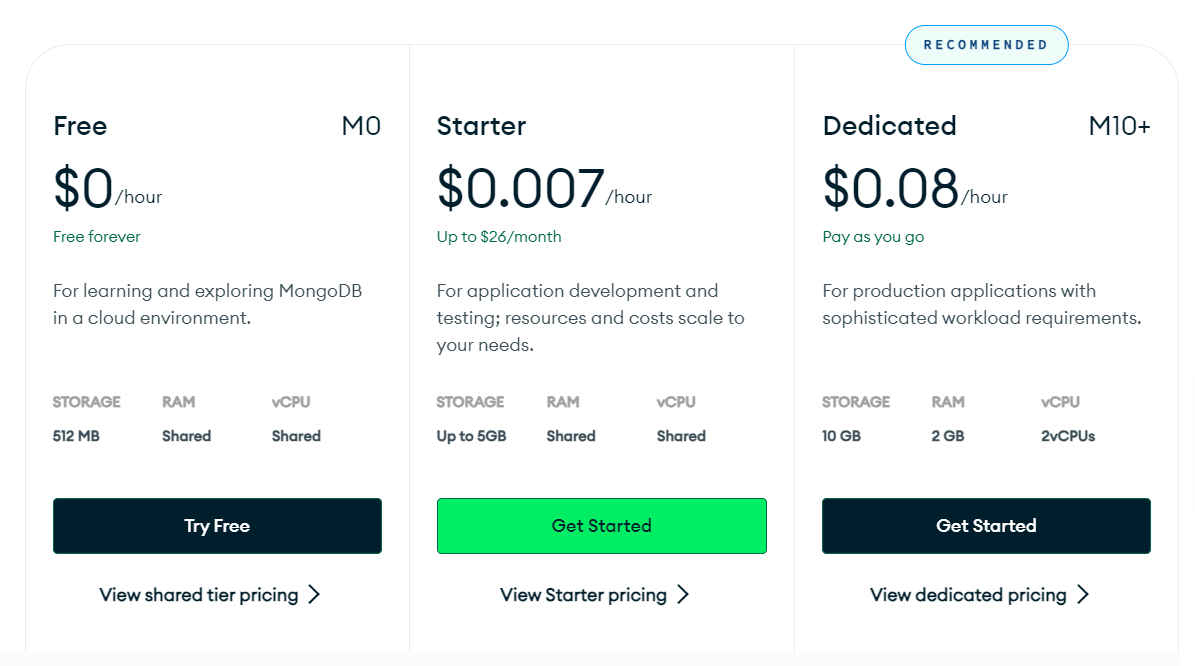
\includegraphics[width=0.8\textwidth]{imatges/mongodb.png} % Ajusta el nom i el camí del fitxer d'imatge
    \caption{El preu del servei MongoDB Atlas.} % Títol de la imatge
    \label{fig:El preu del servei MongoDB Atlas} % Etiqueta per referenciar la imatge
  \end{figure}

\pau{En algun lloc del text hauries de citar la figura, com per exemple ``tal com es veu a la Figura~\ref{fig:El preu del servei MongoDB Atlas}, ...''. Recorda el mateix que abans, també, que en principi encara no has decidit si ho faràs amb MongoDB Atlas (pots fer com abans: ``tal com es veurà al Capítol~\ref{chp:estudi}...''.}



Per determinar la viabilitat econòmica del projecte, és crucial estimar els ingressos potencials i calcular el temps necessari per amortitzar la inversió inicial. A continuació es presenten les estimacions basades en les dades actuals:\\

El cost inicial del projecte es compon de 6.750 € per al desenvolupament de l'aplicació i 5.000 € per al manteniment anual, sumant un total de 11.750 €.\\

Amb una previsió de 1.000 clients, cadascun amb un dipòsit de 1.000 €, el total de dipòsits seria de 1.000.000 €. Aquesta quantitat permetrà realitzar inversions que generaran interessos. Si assumim una taxa d'interès anual del 2\%, els interessos generats seran de 20.000 € cada any.\\

Així, amb aquests guanys d'interessos, la recuperació dels 11.750 € invertits es podria aconseguir en aproximadament 0,6 anys, equivalent a uns 7 mesos. Aquest càlcul indica que, amb una base sòlida de clients i dipòsits, la inversió inicial podria ser amortitzada en un període relativament curt, mostrant així un bon potencial de rendibilitat per al projecte.\\

\pau{Aquí podria estar bé fer una estimació dels ingressos, i així poder dir quan es creu que pot amortitzar-se la inversió inicial, comptant el desenvolupament de l'aplicació i el seu manteniment.}\sudan{corregit}

El sistema de pagament mitjançant codis QR ofereix una solució econòmica en comparació amb els terminals de TPV tradicionals, amb una possible font d'ingressos a través de comissions per transacció i opcions de subscripció per serveis addicionals.




\section{Viabilitat de mercat}
\label{subsec:Viabilitat de mercat}

Amb l'augment de l'ús de pagaments mòbils i la necessitat de solucions de pagament \textit{contactless}, hi ha una demanda creixent per a sistemes de pagament basats en codis QR. Aquesta tendència proporciona una oportunitat significativa per a la nostra aplicació.\\

Encara que hi ha altres solucions de pagament basades en codis QR, el nostre sistema es diferencia per la seva integració fàcil amb altres plataformes i la seva estructura de codi obert, que permet personalització i adaptació a les necessitats específiques dels usuaris.



\pau{Recorda citar la Figura~\ref{fig:Un codi QR de Paypal}; si no, no se sap d'on baixa... Per exemple, just quan dius que hi ha altres solucions basades en codis QR, pots posar entre parèntesis alguna cosa com ``veure, per exemple, la Figura~\ref{fig:Un codi QR de Paypal}, on es mostra un codi QR de PayPal''.}\sudan{corregit}

\begin{figure}[h!] % La posició de la figura pot ser ajustada amb 'h!', 't', 'b', etc.
    \centering
    
\includegraphics[width=0.3\textwidth]{imatges/paypal.png} % Ajusta el nom i el camí del fitxer d'imatge
    \caption{Un codi QR de PayPal.} % Títol de la imatge
    \label{fig:Un codi QR de Paypal} % Etiqueta per referenciar la imatge
  \end{figure}

  La imatge mostrada a la Figura~\ref{fig:Un codi QR de Paypal} és un exemple d'un anunci de PayPal. Com es pot observar, l'anunci destaca la facilitat d'ús del sistema: només cal escanejar el codi QR, efectuar el pagament i continuar amb les activitats diàries. Aquest procés de pagament és extremadament còmode i simplificat per a l'usuari.

\chapter{Metodologia}
\label{chp:metodologia}


\section{Introducció}
\label{subsec: Introducció}

La metodologia utilitzada en aquest projecte és la metodologia àgil, en concret \textbf{Scrum}, tot i que es tracta d'un projecte individual.\\

Les metodologies àgils són un conjunt de principis i pràctiques de gestió de projectes dissenyades per a la flexibilitat i la rapidesa en el desenvolupament de productes. A diferència dels enfocaments tradicionals, que sovint són rígids i seqüencials, les metodologies àgils se centren en la iteració, la col·laboració i l'adaptabilitat. Ofereixen diversos avantatges respecte a les metodologies tradicionals:
\begin{itemize}
    \item \textbf{Adaptabilitat als Canvis}: Les metodologies àgils permeten ajustar els requisits i prioritats al llarg del projecte, mentre que les metodologies tradicionals són més rígides i difícils de modificar un cop el desenvolupament està en marxa.
    \item \textbf{Desenvolupament Iteratiu}: Amb àgil, es treballa en iteracions curtes i incrementals, proporcionant resultats parcials i millorant contínuament el producte. En canvi, les metodologies tradicionals solen seguir un enfocament seqüencial, amb un lliurament complet al final del projecte.
    \item \textbf{Reducció de Riscos}: La revisió contínua i les iteracions àgils ajuden a identificar i abordar problemes abans que es converteixin en grans obstacles, mentre que les metodologies tradicionals poden identificar riscos tardanament, quan ja poden ser més difícils de gestionar.
\end{itemize}


\pau{Pots posar una mica més de context: per exemple, explicar què són les metodologies àgils i quins avantatges tenen respecte metodologies més tradicionals. Pots fer-ho en una subsecció, si vols.}\sudan{corregit}

\section{Scrum}
\label{subsec: Scrum}

Scrum és un marc de treball per a la gestió de projectes, conegut per la seva flexibilitat i per permetre gestionar projectes complexos a través de cicles iteratius de treball anomenats \textit{sprints}. Encara que tradicionalment Scrum està dissenyat per a equips, es van adaptar els seus principis per optimitzar la gestió del temps i els recursos durant el desenvolupament del projecte.\\


L'elecció d'Scrum es va basar en la necessitat de mantenir una alta capacitat de resposta davant els canvis en els requisits i per estructurar el procés de desenvolupament en fases manejables. Scrum va permetre dividir el projecte en \textit{sprints}, cosa que va facilitar la planificació i el seguiment del progrés, assegurant-se que cada fase del projecte es completava abans de passar a la següent.\\

Per a la planificació del projecte, es defineixen \textit{sprints} de dues setmanes, cadascun amb objectius específics que cal complir abans d'iniciar el següent \textit{sprint}. Al principi de cada \textit{sprint}, s'elabora un pla detallat de les tasques a realitzar, prioritzant les més crítiques i assegurant que estan alineades amb els objectius generals del projecte.\\


\begin{figure}[h!] % La posició de la figura pot ser ajustada amb 'h!', 't', 'b', etc.
    \centering
    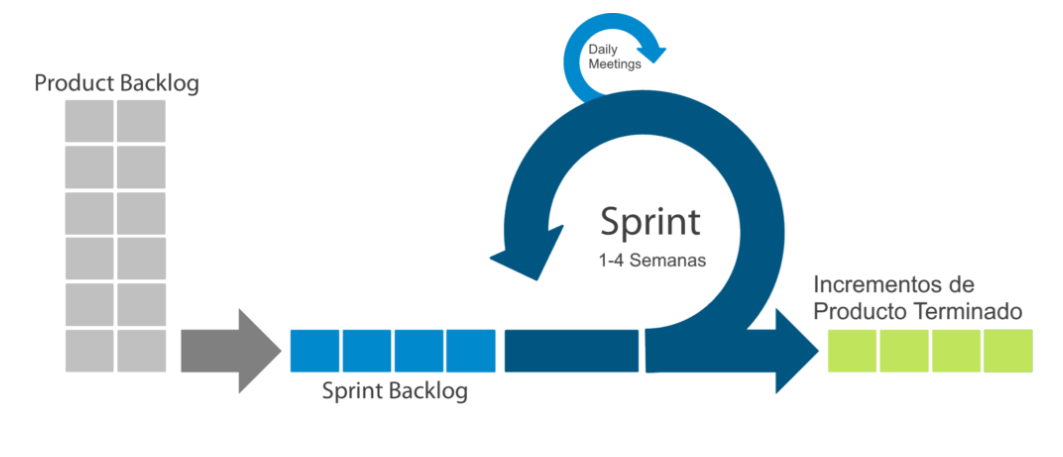
\includegraphics[width=0.8\textwidth]{imatges/scrum.png} % Ajusta el nom i el camí del fitxer d'imatge
    \caption{Sistema de treball Scrum.} % Títol de la imatge
    \label{fig:Sistema de treball Scrum} % Etiqueta per referenciar la imatge
  \end{figure}
  
  \pau{Citar figura al text.}\sudan{corregit}

Tal com es veu en la figura~\ref{fig:Sistema de treball Scrum}, es crea i es gestiona un \textit{product backlog} que llista totes les funcionalitats a desenvolupar. Aquest \textit{backlog} es prioritza d'acord amb la seva importància i la complexitat de la implementació. Cada \textit{sprint} es planifica tenint en compte aquesta llista, garantint que es treballa sempre en les tasques més rellevants per al progrés del projecte.\\

L'ús d'Scrum, adaptat a un entorn individual, va ser fonamental per a la gestió eficient del temps i la consecució dels objectius del projecte. Va permetre que el desenvolupament es realitzés de manera ordenada i progressiva, proporcionant la flexibilitat necessària per fer ajustos sobre la marxa. Aquesta metodologia va resultar especialment útil per mantenir el ritme de treball i assegurar que cada fase del projecte es completés amb èxit abans de passar a la següent.


\section{Adaptació del scrum}
\label{subsec: Adaptació del scrum}

Un cop definida la idea principal de l'aplicació, el següent pas és la seva implementació, que es realitza en les següents fases:

\begin{itemize} 
    \item \textbf{Planificació}: Establir els requisits del projecte, crear un product backlog amb les funcionalitats prioritzades i definir els objectius de cada sprint.
    \item \textbf{Disseny}: Desenvolupar l'arquitectura del sistema i el disseny de la interfície d'usuari, amb revisions contínues basades en el feedback rebut. 
    \item \textbf{Desenvolupament}: Implementar les funcionalitats en sprints curts, completant tasques específiques i ajustant segons les necessitats identificades durant el procés. 
    \item \textbf{Revisió i ajustament}: Realitzar revisió per avaluar el treball completat i ajustar les tasques futures. Utilitzar les retrospectives per millorar el procés de desenvolupament. 
    \item \textbf{Entrega}: Lliurar els resultats parcials al final de cada sprint, permetent una validació progressiva i realitzant ajustaments abans de la finalització completa del projecte
\end{itemize}

En Scrum, el procés de desenvolupament permet realitzar canvis en qualsevol moment. Aquesta flexibilitat és una de les principals avantatges, ja que ens permet adaptar-nos de manera contínua als nous requisits. L'enfocament àgil facilita l'ajustament dels objectius i les funcionalitats del projecte al llarg del seu desenvolupament, assegurant que el producte final s'alineï amb les necessitats canviants i les expectatives dels clients. Aquesta capacitat d'adaptació contínua garanteix que el projecte pugui respondre eficaçment a les variacions del mercat i a les noves oportunitats que puguin sorgir.



\pau{Podria estar bé explicar una mica com s'ha adaptat aquesta metodologia al projecte actual, explicant-ne una mica les fases, per exemple (planificació, disseny, desenvolupament...). També podries fer-ho en una subsecció, si vols.}\sudan{corregit}



\chapter{Planificació}
\label{chp:planificació}

\section{Introducció}
\label{sec:Introducció}

El següent pla de planificació ofereix una visió clara del procés de desenvolupament del projecte, destacant les etapes clau, el temps assignat i els resultats esperats, així com l'aplicació de la metodologia Scrum per gestionar el projecte de manera àgil.



\section{Desenvolupament}

El procés de creació i construcció del producte de programari inclou les següents tasques:

\begin{enumerate}
  \item \textbf{Anàlisi de requisits}:
  \begin{itemize}
      \item Revisar els requisits del projecte.
      \item Establir especificacions detallades per al desenvolupament.
  \end{itemize}

  \item \textbf{Disseny}:
  \begin{itemize}
      \item Crear l'arquitectura del sistema.
      \item Dissenyar les interfícies d'usuari i les interaccions.
      \item Definir les estructures de dades i les lògiques d'operació.
  \end{itemize}

  \item \textbf{Codificació}:
  \begin{itemize}
      \item Escriure el codi font segons les especificacions.
      \item Implementar les funcionalitats del sistema.
      \item Desenvolupar codi de \textit{back end} i \textit{front end}. 
      \pau{Teòricament encara no has decidit les eines: jo potser diria directament ``codi de \textit{back end} i \textit{front end}, sense especificar.}\sudan{corregit}
  \end{itemize}

  \item \textbf{Proves}:
  \begin{itemize}
      \item Crear i executar proves per verificar la funcionalitat de cada component.
      \item Corregir errors detectats durant les proves.
  \end{itemize}

  \item \textbf{Revisió de codi i millores}:
  \begin{itemize}
      \item Realitzar revisions de codi per assegurar la qualitat i el compliment dels estàndards.
  \end{itemize}

  \item \textbf{Documentació}:
  \begin{itemize}
      \item Elaborar memòria sobre l'arquitectura, el disseny i el codi.
  \end{itemize}

  \item \textbf{Manteniment i actualitzacions}
    \begin{itemize}
        \item Realitzar manteniment regular del sistema per assegurar la seva funcionalitat.
        \item Implementar actualitzacions i millores basades en \textit{feedback} i nous requisits.
    \end{itemize}
\end{enumerate}



El Diagrama de Gantt~\ref{fig:Diagrama de Gantt} proporciona una visió detallada del calendari del projecte, desglossant les diferents fases i tasques previstes. Aquesta eina visual ofereix una visió general clara del progrés del projecte, facilitant tant la gestió del temps com l'assignació de recursos. Mitjançant el diagrama, és possible identificar les dates clau i controlar l’avanç de les tasques, ajudant així a assegurar que el projecte es mantingui en el camí correcte per a una finalització exitosa.

\begin{figure}[h!] % La posició de la figura pot ser ajustada amb 'h!', 't', 'b', etc.
    \centering
    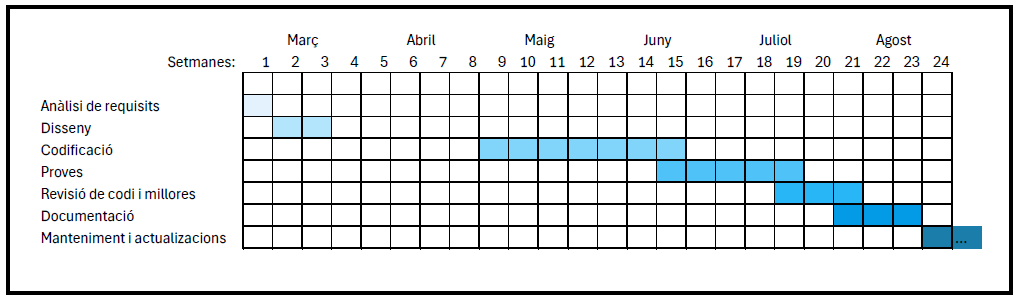
\includegraphics[width=1\textwidth]{imatges/gantt.png} % Ajusta el nom i el camí del fitxer d'imatge
    \caption{Diagrama de Gantt} % Títol de la imatge
    \label{fig:Diagrama de Gantt} % Etiqueta per referenciar la imatge
  \end{figure}

\pau{Jo transformaria aquesta taula en un diagrama de Gantt, que és molt més visual (la columna ``Resultats'' no cal). Abans de posar el diagrama, introdueix-lo amb una mica de text.}\sudan{corregit}

\pau{També faria que tot plegat fos una secció, i no una subsecció.}\sudan{corregit}



\chapter{Marc de treball i conceptes previs}
\label{chp:marcdetreball}


\section{Introducció}
\label{subsec:Introducció}

En aquest capítol es tractaran els coneixements necessaris per desenvolupar correctament una aplicació bancària que utilitza codis QR per realitzar operacions. En resum, és important entendre com funciona el codi QR, especialment en relació amb com emmagatzemar el contingut. A més, cal disposar de coneixements sobre arquitectura i desenvolupament de programari per aportar valor a l'aplicació.

\subsection{Propòsit}
\label{subsec: Propòsit}

\pau{Potser afegiria ``i conceptes clau'' al títol de la subsecció.}\sudan{corregit}

L'objectiu de l'aplicació és proporcionar una plataforma senzilla, escalable i potent per gestionar els pagaments i cobraments mitjançant codis QR. Tant els clients com els comerciants tindran accés a funcionalitats i permisos dins de l'aplicació, permetent-los configurar els seus sistemes de pagament o cobrament, establir opcions disponibles, ajustar els límits de transacció i altres configuracions relacionades. A més de facilitar les compres, l'aplicació permetrà als usuaris realitzar transferències entre amics i familiars, oferint així una solució versàtil per a diverses necessitats financeres quotidianes.\\

Per tant, en una sola aplicació, els usuaris podran controlar totes les transaccions que es realitzin, alhora que tindran la capacitat d'aplicar canvis i modificacions segons les seves necessitats i preferències.\\


\subsection{Conceptes clau}
\label{subsec: Conceptes clau}

A continuació, es presenta una llista amb les parts fonamentals que defineixen el funcionament de l'aplicació:

\begin{itemize}
    \item \textbf{App}: L'aplicació es pot concebre com una entitat bancària en si mateixa, on els seus usuaris actuen com a clients que poden tant rebre com enviar pagaments. 
    \item \textbf{Usuari Client}: L'usuari client és la persona que utilitza l'aplicació per realitzar pagaments o cobraments.
    \item \textbf{Usuari Administrador}: L'usuari administrador és qui gestiona l'aplicació, configurant els sistemes de pagament i supervisant les transaccions, comptes i també els usuaris.
    \item \textbf{Transacció}: Les transaccions es fan entre comptes bancaris, independentment dels usuaris. No es pot fer una transacció dins del mateix compte, però sí que poden ser entre comptes del mateix client.
    \item \textbf{QR de pagament}: Per a cada compte, només hi ha un codi QR actiu, ja que aquests estan xifrats per garantir la seguretat. Cada vegada que es genera un nou codi QR, la clau de desxifratge s’actualitza. A més, els codis QR són d'ús únic i caduquen després d'un temps determinat. Tots aquests processos es duen a terme per reforçar la protecció.
    \item \textbf{QR de cobrament}: El codi QR de cobrament és més senzill que el de pagament, ja que presenta menys restriccions. A diferència del codi QR de pagament, el de cobrament no està xifrat ni caduca, i es pot utilitzar tantes vegades com es desitgi.
    \item \textbf{Activat/Desactivar Usuari client}: Un usuari pot canviar l'estat del seu compte per si mateix o mitjançant un administrador. Quan el usuari està desactivat, l'usuari no podrà realitzar cap acció ni visualitzar informació, encara que podrà rebre cobraments.
    \item \textbf{Activar/Desactivar Compte}: Un compte pot canviar el seu estat per si mateix o mitjançant un administrador. Quan el compte està desactivat, l'usuari no podrà generar codis QR de pagament ni fer pagaments amb el compte desactivat. Altres operacions seguiran igual.
    \item \textbf{Dictionary}: Cada cop que l'usuari genera un codi QR, tota la informació es guarda en un Diccionary. Quan el codi és escanejat, el sistema consulta internament aquest Diccionary per obtenir les dades necessàries, com el compte d'origen i l'import.
    \item \textbf{Codi QR}: El codi QR és un element clau de l'aplicació, utilitzat per comunicar informació entre clients.
\end{itemize}

\pau{Pots pensar altres conceptes clau com ara ``transacció'', ``QR de pagament'', ``QR de cobrament''...}\sudan{corregit}



\subsection{Codi QR}
\label{subsec: Codi QR}

Els codis QR (Quick Response) van ser desenvolupats al Japó a mitjans dels anys 90. És un tipus de codi de barres bidimensional que pot emmagatzemar una gran quantitat d'informació en un espai reduït. Aquest codi es pot escanejar fàcilment amb la càmera d'un telèfon mòbil o amb dispositius específics, permetent accedir a la informació que conté de manera ràpida i senzilla.\\

La Figura~\ref{fig:Imatge d'un codi QR} mostra un codi QR. Es pot escanejar amb la càmera del mòbil i conté text emmagatzemat en el seu interior. El codi QR té tres quadrats grans en les cantonades, que ajuden a posicionar-lo correctament. La resta dels quadrats són en general de dos colors: negre (1) i blanc (0). Aquests colors formen un patró que representa informació en format binari, que posteriorment es converteix en text.

\begin{figure}[h!] % La posició de la figura pot ser ajustada amb 'h!', 't', 'b', etc.
    \centering
    
\includegraphics[width=0.3\textwidth]{imatges/qr2.png} % Ajusta el nom i el camí del fitxer d'imatge
    \caption{Imatge d'un codi QR.} % Títol de la imatge
    \label{fig:Imatge d'un codi QR} % Etiqueta per referenciar la imatge
  \end{figure}

Els codis QR s'han popularitzat per la seva versatilitat i eficiència. En aplicacions de pagaments i cobraments, els codis QR ofereixen una manera ràpida i segura de transferir informació, com per exemple detalls de pagament o d'una transacció específica. L'usuari simplement escaneja el codi amb el seu dispositiu i la informació es transmet instantàniament, eliminant la necessitat d'entrar dades manualment, reduint errors i accelerant el procés de transacció.\\


\chapter{Requisits del sistema}
\label{chp:requisits}




\section{Introducció}
\label{subsec:Introducció}

Aquest capítol tractarà l'especificació de requisits del sistema per al programari que s'està desenvolupant. Es fixaran les bases del que es desenvoluparà, tenint en compte les necessitats dels usuaris, així com els requisits funcionals i no funcionals.\\

Els requisits funcionals es defineixen com les funcionalitats bàsiques del sistema. Aquests requisits especificen què ha de fer el sistema, descrivint les accions que ha de ser capaç de realitzar i les operacions que ha de suportar. Tots els requisits exposats en aquesta secció es consideren essencials i el sistema es consideraria incomplet si no complís aquests requisits.\\

Els requisits no funcionals, d'altra banda, defineixen les qualitats o atributs del sistema, com ara el seu rendiment, seguretat, escalabilitat i usabilitat.




\subsection{Els requisits funcionals}
\label{subsec:Els requisits funcionals}


La funcionalitat bàsica de l'aplicació que es presenta és fer transferències de diners entre dues usuaris. Seria una funció semblant al que permet la tecnologia ``Bizum'', però incorporant el servei de pagament/cobrament mitjançant codis QR. 

En l'apartat de bibliografia es detallen amb més precisió les informacions sobre BIZUM.

\begin{itemize}
    \item https://bizum.es/
\end{itemize}

\pau{Aquí és una bona oportunitat per afegir un ítem a la bibliografia relacionat amb Bizum.}\sudan{Alguna cosa així??}

D'altra banda, el Bizum està vinculat a un número de telèfon, mentre que l'aplicació que es presenta es vincularà a un número de compte bancari. Cada compte bancari serà capaç de generar codis QR per a cobraments o, a la inversa, serà capaç de llegir codis QR per a efectuar pagaments.\\



\textbf{Gestió d'usuaris clients:}
\begin{itemize}
    \item \textbf{RF-1.} Els usuaris clients han de poder registrar-se amb informació bàsica.
    \item \textbf{RF-2.} Els usuaris clients han de poder iniciar sessió a l'aplicació utilitzant les seves credencials.
    \item \textbf{RF-3.} Els usuaris clients han de poder modificar la contrasenya d'accés, proporcionant la contrasenya antiga.
    \item \textbf{RF-4.} Els usuaris clients han de poder donar-se de baixa ells mateixos.
    \item \textbf{RF-5.} Els usuaris clients han de poder configurar els seus comptes, incloent l'estat, la descripció i el límit màxim per transaccions, entre altres opcions.
\end{itemize}


\textbf{Gestió d'usuaris administradors:}
\begin{itemize}
    \item \textbf{RF-6.} Els usuaris administradors han de poder registrar-se amb informació bàsica, però caldrà disposar de les credencials d'un altre administrador.
    \item \textbf{RF-7.} Els usuaris administradors han de poder iniciar sessió a l'aplicació utilitzant les seves credencials.
    \item \textbf{RF-8.} Els usuaris administradors han de poder modificar la contrasenya d'accés, proporcionant la seva contrasenya antiga.
    \item \textbf{RF-9.} Els usuaris administradors han de poder donar una nova contrasenya d'accés a l'usuari client, sense que calgui proporcionar la contrasenya antiga.
    \item \textbf{RF-10.} Els usuaris administradors han de poder donar-se de baixa ells mateixos (excepte l'usuari ``admin'').
\end{itemize}


\textbf{Operacions d'usuari administrador:}
\begin{itemize}
    \item \textbf{RF-11.} Els usuaris administradors han de poder visualitzar tots els usuaris clients i tots els moviments associats als seus comptes.
    \item \textbf{RF-12.} Els usuaris administradors han de poder veure tots els usuaris administradors i tots els moviments associats a cadascun d'ells.
    \item \textbf{RF-13.} Els usuaris administradors han de poder gestionar tant els usuaris clients com els seus comptes.
\end{itemize}


\textbf{Operacions de transaccions d'usuari client:}
\begin{itemize}
    \item \textbf{RF-14.} Els usuaris clients han de poder generar un codi QR únic associat al seu compte per rebre pagaments i cobraments, amb o sense un preu definit.
    \item \textbf{RF-15.} Els usuaris clients han de poder escanejar codis QR generats per altres usuaris per fer pagaments i cobraments, introduint el preu si no està definit prèviament.
    \item \textbf{RF-16.} Els usuaris poden fer transaccions mitjançant l'entrada manual del número de compte del destinatari, en cas que la càmera no funcioni.

\end{itemize}

\textbf{Funcionalitats addicionals:}
\begin{itemize}
    \item \textbf{RF-17.} S'ha de generar un \textit{log} que registri tots els moviments tant de l'usuari client com de l'usuari administrador.
\end{itemize}


\textbf{Integracions i serveis complementaris:}
\begin{itemize}
        \item \textbf{RF-18.} S'ha de poder canviar el color de fons de l'aplicació.
\end{itemize}


\subsection{Els requisits no funcionals}
\label{subsec:Els requisits no funcionals }

\textbf{Els requisits no funcionals són:}
\begin{itemize}
    \item \textbf{RNF-1.} L'aplicació ha de ser ràpida i eficient, amb temps de càrrega mínims i una resposta àgil a les interaccions de l'usuari.
    \item \textbf{RNF-2.} S'han d'implementar mesures de seguretat robustes, com l'autenticació i el xifrat de dades, per protegir la informació personal i financera dels usuaris. \pau{Això seria requisit no funcional!}\sudan{corregit}
    \item \textbf{RNF-3.} L'aplicació ha de poder gestionar un alt volum de transaccions i usuaris concurrents, amb la capacitat d'escalar horitzontalment segons sigui necessari.
    \item \textbf{RNF-4.} La interfície d'usuari ha de ser intuïtiva i fàcil d'utilitzar, amb un disseny net i clar que permeti als usuaris realitzar les seves tasques de manera eficient.
    \item \textbf{RNF-5.} L'aplicació ha de ser compatible amb una varietat de dispositius i sistemes operatius, incloent telèfons mòbils, tauletes. \pau{Per a ordinadors també?}\sudan{corregit}
    \item \textbf{RNF-6.} S'han d'implementar pràctiques de seguretat sòlides per protegir la integritat i la confidencialitat de les dades dels usuaris, així com per prevenir frau i atacs cibernètics.

\end{itemize}


\subsection{Matriu de dependències de requisits}
\label{Matriu de dependències de requisits}

A continuació presenta una taula~\ref{fig:Matriu de dependències de requisits funcionals} que il·lustra les relacions entre els diferents requisits del projecte. Aquesta matriu és fonamental per entendre com cada requisit es connecta i depèn d'altres, facilitant així la gestió de canvis i l'assegurament de la coherència durant tot el cicle de vida del projecte.\\

A través d'aquesta matriu, es poden identificar clarament les interdependències, cosa que permet una millor planificació i implementació dels requisits:

\begin{itemize}
    \item Els requisits RF\_1 i RF\_6 són operacions de registre.
    \item Els requisits RF\_3, RF\_4, RF\_5, RF\_14, RF\_15 i RF\_16 són operacions de l'usuari client; per dur-les a terme, cal que l'usuari client estigui identificat.
    \item Els requisits RF\_8, RF\_9, RF\_10, RF\_11, RF\_12 i RF\_13 són operacions de l'usuari administrador; per dur-les a terme, cal que l'usuari administrador estigui identificat.
    \item Finalment, els requisits RF\_17 i RF\_18 són requisits complementaris, i requereixen que tant el client com l'administrador estiguin autenticats.
\end{itemize}


\pau{Aquí quedaria molt millor una matriu de veritat. Exemple ràpid trobat a internet: \url{http://wiki.doing-projects.org/images/4/4b/DSM.PNG}. Llavors pots complementar la matriu amb la taula que tens, on expliques la descripció de les dependències.}\sudan{corregit}


\begin{figure}[h]
    \centering
    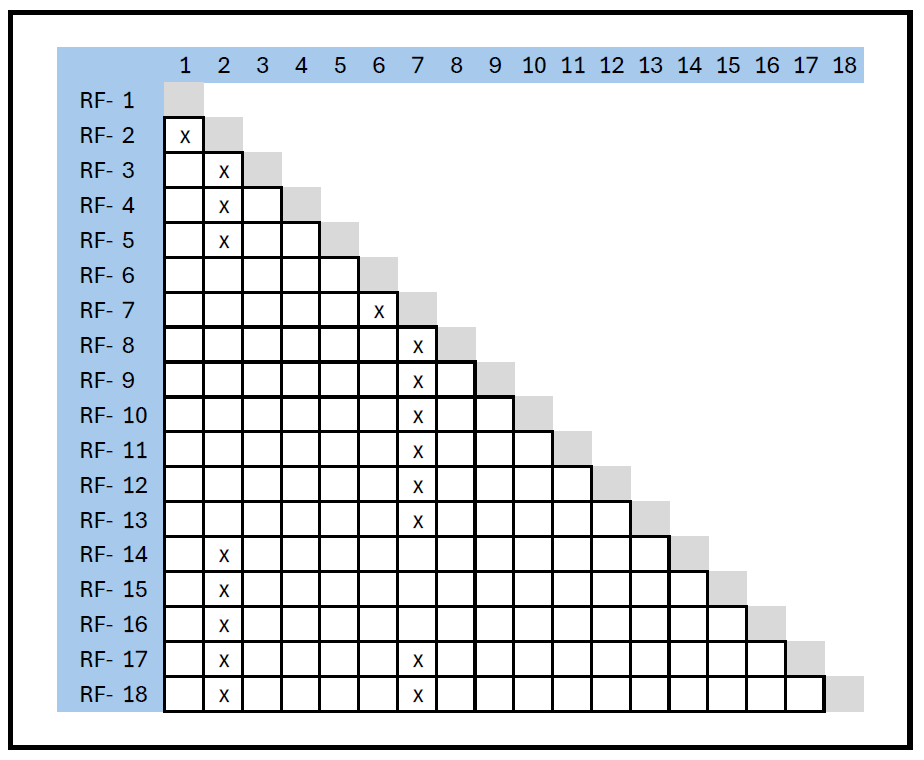
\includegraphics[width=0.9\textwidth]{imatges/taula dependencies.png}
    \caption{Matriu de dependències de requisits funcionals}
    \label{fig:Matriu de dependències de requisits funcionals}
\end{figure}



    

\chapter{Estudi i decisions}
\label{chp:estudi}
\sudan{Tornat a fer}

\section{Introducció}
\label{sec:Introducció}

En aquest capítol es presenten els diferents aspectes que s'han considerat per escollir les tecnologies utilitzades en el desenvolupament del sistema. Les decisions sobre el maquinari, les llibreries i el programari s'han pres tenint en compte criteris de rendiment, compatibilitat, facilitat d'ús i mantenibilitat a llarg termini.
 \pau{Potser millor ``... per escollir les tecnologies utilitzades per desenvolupar el sistema''.}\sudan{corregit}


 \section{Maquinari}
 \label{sec: Maquinari}

Per al desenvolupament del projecte, s'ha utilitzat un portàtil Lenovo ThinkPad amb les següents especificacions:

\begin{itemize}
    \item Processador: Intel Core i7
    \item Memòria RAM: 16 GB DDR4
    \item Disc dur: SSD de 512 GB
    \item Sistema operatiu: Windows 10
\end{itemize}

Aquest maquinari s'ha seleccionat per la seva fiabilitat i capacitat de processament, que són essencials per gestionar l'execució simultània de diverses eines de desenvolupament.



\section{Front-end}
\label{sec: Front-end}

El \textit{front end} es refereix a la part del desenvolupament d'una aplicació o lloc web que interactua directament amb els usuaris. En termes simples, és tot el que els usuaris veuen i amb el que interactuen en una aplicació o pàgina web. Inclou el disseny i la implementació de la interfície d'usuari (UI), que comprèn elements com ara botons, menús, pàgines i imatges.\\

Per al desenvolupament de front-end d'aplicacions mòbils, hi ha diverses tecnologies i eines que poden ser utilitzades, depenent de les necessitats específiques del projecte, com la plataforma objectiu, els requisits d'usuari i el rendiment desitjat. 

\subsection{Tecnologies més conegudes}
\label{subsec: Tecnologies més conegudes}

A continuació, es detallen algunes de les tecnologies més conegudes i populars per al desenvolupament de front-end en aplicacions mòbils:

\begin{itemize}
    \item \textbf{Flutter}
    \begin{itemize}
        \item \textbf{Descripció:} Flutter és un framework creat per Google per al desenvolupament d'interfícies d'usuari. Permet crear aplicacions mòbils nadiues per a iOS i Android utilitzant un sol codi font, escrit en el llenguatge Dart. Flutter proporciona una gran varietat de widgets personalitzables que faciliten el disseny d'interfícies d'usuari atractives i de rendiment alt.
        \item \textbf{Avantatges:} Disseny consistent entre plataformes, rendiment elevat gràcies a la compilació a codi nadiu, i un ampli conjunt de widgets personalitzables.
    \end{itemize}

    \item \textbf{React Native}
    \begin{itemize}
        \item \textbf{Descripció:} React Native és un framework creat per Facebook que permet el desenvolupament d'aplicacions mòbils utilitzant JavaScript i React. Ofereix components nadius que es poden utilitzar per crear aplicacions per a ambdues plataformes, iOS i Android, amb un codi base compartit.
        \item \textbf{Avantatges:} Compartició de codi entre plataformes, gran comunitat i ecosistema amb moltes biblioteques i recursos, i capacitat d'integrar-se amb codi nadiu quan sigui necessari.
    \end{itemize}

    \item \textbf{Xamarin}
    \begin{itemize}
        \item \textbf{Descripció:} Xamarin és una plataforma de Microsoft per al desenvolupament d'aplicacions mòbils utilitzant C\# i \.NET\. Permet als desenvolupadors crear aplicacions nadiues per a iOS i Android amb un sol codi font, compartint gran part del codi entre plataformes.
        \item \textbf{Avantatges:} Integració amb l'ecosistema \.NET i Visual Studio, reutilització significativa del codi entre plataformes, i accés a les API nadiues i funcions específiques del dispositiu.
    \end{itemize}

    \item \textbf{Ionic}
    \begin{itemize}
        \item \textbf{Descripció:} Ionic és un framework basat en HTML5 per al desenvolupament d'aplicacions mòbils híbrides. Utilitza tecnologies web com HTML, CSS i JavaScript, i es basa en Angular o Vue.js per gestionar l'arquitectura de l'aplicació. Ionic permet crear aplicacions que es poden executar en qualsevol dispositiu mitjançant un navegador web o com a aplicacions híbrides mitjançant Cordova o Capacitor.
        \item \textbf{Avantatges:} Desenvolupament ràpid amb tecnologies web familiars, capacitat d'exportar a diverses plataformes amb un sol codi base, i gran biblioteca de components d'interfície d'usuari.
    \end{itemize}
    
\end{itemize}

\subsection{Tecnologia Escollida: Flutter}
\label{subsec: Tecnologia Escollida: Flutter}

En aquest projecte, s'ha escollit \textbf{Flutter} com a framework per al desenvolupament del front-end de l'aplicació mòbil. A continuació, es detallen les raons per les quals Flutter ha estat seleccionat, així com els avantatges clau que ofereix aquest framework, especialment en comparació amb altres opcions comunes:

\begin{itemize}
    \item \textbf{Rendiment Elevat:} Flutter ofereix un rendiment destacat gràcies a la seva arquitectura basada en la compilació a codi nadiu. A diferència de les solucions híbrides com React Native o Ionic, que utilitzen una capa intermitja per comunicar-se amb el sistema operatiu, Flutter compila directament a codi nadiu. Aquesta característica millora la velocitat d'execució i la resposta davant les accions dels usuaris.

    \item \textbf{Disseny Consistent:} Flutter proporciona una experiència visual i funcional uniforme tant en dispositius Android com iOS gràcies als seus widgets personalitzables. Això és una millora respecte a les tecnologies com React Native, que poden requerir ajustaments addicionals per garantir que l'aplicació sigui coherent entre plataformes. Flutter permet als desenvolupadors mantenir un disseny consistent sense necessitat de personalitzar excessivament el codi per a cada plataforma.

    \item \textbf{Productivitat Augmentada:} Flutter utilitza el \textbf{llenguatge Dart}, que facilita l'escriptura de codi de manera eficient. La funcionalitat de *hot reload* de Flutter permet als desenvolupadors veure els canvis en temps real sense haver de reiniciar l'aplicació completa. Aquesta característica és superior a les eines de desenvolupament d'altres frameworks com Xamarin, on el procés de reinici i recompilació pot ser més llarg.

    \item \textbf{Suport Actiu i Comunitat:} Flutter compta amb un suport actiu per part de Google i una comunitat en creixement que proporciona recursos i solucions per a problemes comuns. Aquesta comunitat en creixement i el suport continuat asseguren que Flutter continuï evolucionant i millorant. Comparat amb frameworks com Xamarin o Ionic, que poden tenir comunitats més petites o menys activament suportades, Flutter ofereix un ecosistema més robust i dinàmic.
\end{itemize}

Amb aquests avantatges, Flutter es presenta com una opció ideal per al desenvolupament d'aplicacions mòbils que necessiten un rendiment excel·lent, una interfície d'usuari atractiva i una alta eficiència en el procés de desenvolupament. La seva arquitectura i funcionalitats el diferencien clarament d'altres tecnologies i el converteixen en una elecció destacada per a projectes amb requisits exigents.


\pau{Caldria explicar una mica els avantatges de cada tecnologia que es presenta respecte a altres alternatives, justificant-ne així l'elecció.}\sudan{corregit}


\subsection{IDE Escollida: Android Studio}
\label{subsec:IDE Escollida: Android Studio}

Per al desenvolupament d'aplicacions amb Flutter, hi ha diversos entorns de desenvolupament integrats (IDE) disponibles. En aquest projecte, s'ha escollit \textbf{Android Studio} com a IDE per implementar la part client. Android Studio és l'entorn de desenvolupament integrat oficial per a aplicacions Android, creat per Google. Aquest IDE ofereix un conjunt complet d'eines dissenyades per facilitar la creació i gestió d'aplicacions destinades a dispositius Android.\\

Un aspecte destacat d'Android Studio és l'emulador integrat, que permet provar les aplicacions en dispositius simulats sense necessitat de tenir un dispositiu físic. L'emulador simula diverses configuracions de dispositius Android, com ara diferents mides de pantalla i versions del sistema operatiu. Això permet als desenvolupadors observar com es comporta l'aplicació en una gamma de condicions i configuracions diverses. L'ús de l'emulador facilita la depuració i les proves, oferint una manera ràpida i flexible de verificar el funcionament de l'aplicació abans del desplegament final.



\section{Back-end}
\label{sec: Back-end}

El \textit{back end} és la part de l'arquitectura d'una aplicació que opera al servidor, gestionant la lògica de negoci, el processament de dades i la comunicació amb altres serveis. La seva funció principal és assegurar que l'aplicació funcioni correctament, processant les sol·licituds dels usuaris i gestionant les operacions internes necessàries per proporcionar una resposta adequada.


\subsection{Tecnologies més conegudes}
\label{subsec: Tecnologies més conegudes}


Per al desenvolupament del backend d'una aplicació mòbil, hi ha diverses tecnologies àmpliament utilitzades que ofereixen diferents avantatges segons les necessitats específiques del projecte. A continuació es presenten algunes de les tecnologies més conegudes:

\begin{itemize}
    \item \textbf{Node.js}: Node.js és una plataforma de servidor basada en el motor JavaScript V8 de Google Chrome. Permet als desenvolupadors escriure el backend de les aplicacions utilitzant JavaScript. 
    \begin{itemize}
        \item \textbf{Avantatges:}
        \begin{itemize}
            \item \textbf{Asíncron i No Bloquejant:} Permet manejar moltes connexions simultànies amb alta eficiència.
            \item \textbf{Ecosistema Gran:} Té un ecosistema extens amb nombroses llibreries i paquets disponibles a través de npm (Node Package Manager).
            \item \textbf{Full Stack JavaScript:} Permet usar JavaScript tant al frontend com al backend, facilitant la integració entre ambdós.
        \end{itemize}
    \end{itemize}
    
    \item \textbf{Ruby on Rails}: Ruby on Rails, sovint anomenat Rails, és un framework de desenvolupament web en Ruby que utilitza el patró Model-View-Controller (MVC).
    \begin{itemize}
        \item \textbf{Avantatges:}
        \begin{itemize}
            \item \textbf{Desenvolupament Ràpid:} Facilita el desenvolupament ràpid gràcies a la seva estructura de convenció sobre configuració.
            \item \textbf{Facilitat d'Ús:} Ofereix una sintaxi neta i llegible que simplifica el codi.
            \item \textbf{Comunitat Activa:} Té una comunitat activa amb moltes gems (llibreries) disponibles per afegir funcionalitats.
        \end{itemize}
    \end{itemize}

    \item \textbf{Spring Boot}: Spring Boot és un framework en Java que facilita el desenvolupament d'aplicacions empresarials basades en Spring, proporcionant una configuració mínima i opcions de desplegament senzilles.
    \begin{itemize}
        \item \textbf{Avantatges:}
        \begin{itemize}
            \item \textbf{Configuració Automàtica:} Ofereix configuració automàtica basada en les dependències incloses al projecte.
            \item \textbf{Escalabilitat:} És adequat per a aplicacions d’empresa amb grans requisits d'escalabilitat.
            \item \textbf{Integració:} Facilita la integració amb altres tecnologies i serveis de Spring.
        \end{itemize}
    \end{itemize}

    \item \textbf{Express.js}: Express.js és un framework minimalista i flexible per a Node.js que proporciona un conjunt de característiques per al desenvolupament web i de backend.
    \begin{itemize}
        \item \textbf{Avantatges:}
        \begin{itemize}
            \item \textbf{Simplicitat i Flexibilitat:} Permet construir aplicacions ràpidament amb una arquitectura senzilla i flexible.
            \item \textbf{Middleware:} Ofereix suport per a middleware, facilitant la gestió de les sol·licituds HTTP.
            \item \textbf{Popularitat:} Amplament utilitzat en combinació amb MongoDB i Angular/React per a desenvolupaments full-stack (conegut com a MEAN/MERN stack).
        \end{itemize}
    \end{itemize}


    \item \textbf{GraphQL}: GraphQL és una consulta d'API i llenguatge de manipulació de dades desenvolupat per Facebook. Ofereix una alternativa a REST per a la consulta i manipulació de dades.
    \begin{itemize}
        \item \textbf{Avantatges:}
        \begin{itemize}
            \item \textbf{Consultes Flexibles:} Permet als clients sol·licitar exactament les dades que necessiten, evitant la sobrecàrrega de dades.
            \item \textbf{Tipat Fort:} Utilitza un sistema de tipus fort que facilita el desenvolupament i depuració.
            \item \textbf{Evolució de l'API:} Permet evolucionar l'API sense afectar les consultes existents.
        \end{itemize}
    \end{itemize}
\end{itemize}
La creació d'APIs (Interfícies de Programació d'Aplicacions) és fonamental per permetre la comunicació entre el servidor i els clients.

\pau{Igual que abans, caldria explicar una mica els avantatges de cada tecnologia que es presenta respecte a altres alternatives, justificant-ne així l'elecció.}


\subsection{Tecnologia Escollida: GraphQL}
\label{subsec: Tecnologies Escollida: GraphQL}

En el desenvolupament del backend de l'aplicació mòbil, aqueste projecte utilitza GraphQL com a tecnologia principal. GraphQL és un llenguatge de consulta d'API desenvolupat per Facebook que ofereix diverses avantatges respecte a altres tecnologies de backend tradicionals com REST.\\

Una de les principals avantatges de GraphQL és la seva capacitat per proporcionar consultes flexibles. A diferència de les API REST, on cada endpoint retorna un conjunt fix de dades, GraphQL permet als clients especificar exactament quins camps volen recuperar. Això evita la sobrecàrrega de dades i optimitza la comunicació entre el client i el servidor, ja que només es transfereixen les dades necessàries per a cada sol·licitud. Aquesta característica és especialment valuosa en entorns mòbils, on l'ús eficient de l'ample de banda i la velocitat de resposta són essencials.\\

A més, GraphQL utilitza un sistema de tipus fort i un esquema ben definit que facilita tant el desenvolupament com la depuració. Els tipus de dades i les operacions disponibles estan clarament especificats en l’esquema, cosa que permet una millor validació i documentació automàtica de l'API. Això no només accelera el desenvolupament, sinó que també millora la qualitat i la mantenibilitat del codi.\\

Un altre avantatge important de GraphQL és la seva capacitat per evolucionar l'API de manera flexible. Amb GraphQL, es poden afegir nous camps i tipus de dades a l'API sense afectar les consultes existents. Això facilita l'evolució contínua de l'API sense interrupcions per als clients actuals, permetent un desplegament més suau de noves funcionalitats.\\

En comparació amb tecnologies com REST, que requereixen múltiples endpoints per accedir a diferents recursos, GraphQL simplifica l'arquitectura de l'API. Amb un sol endpoint, es poden realitzar diverses consultes i mutacions, cosa que redueix la complexitat del sistema i millora la seva eficiència.\\



\subsection{Codi obert per implementar servidors GraphQL: Apollo Server}
\label{Codi obert per implementar servidors GraphQL: Apollo Server}


Apollo Server és una biblioteca poderosa i versàtil que simplifica la creació i gestió de servidors GraphQL, oferint una interfície intuïtiva i un ecosistema integrat que facilita el desenvolupament.\\

Un dels seus punts forts més destacats és la seva completa compatibilitat amb els estàndards i especificacions de GraphQL, garantint que les aplicacions creades amb aquesta tecnologia segueixin les millors pràctiques i funcionin de manera òptima en qualsevol entorn GraphQL. Entre les seves característiques avançades, destaquen la gestió de subscripcions per a dades en temps real, el suport per a directives personalitzades i una gestió eficient de la memòria cau.\\

Distribuït a través de npm (Node Package Manager), Apollo Server és fàcil d'instal·lar i actualitzar, la qual cosa permet als desenvolupadors integrar-lo ràpidament en els seus projectes. Aquesta facilitat d'ús és un factor clau per al seu èxit en entorns de desenvolupament moderns.\\

Finalment, Apollo Server és altament configurable, permetent als desenvolupadors adaptar-lo a les necessitats específiques del projecte. Aquesta flexibilitat es manifesta en la seva capacitat per funcionar amb qualsevol servidor HTTP, facilitant la seva integració en arquitectures existents sense necessitat de realitzar canvis significatius.

\subsection{Llenguatge Escollit: TS}
\label{subsec:Llenguatge Escillit: TS}

El llenguatge de programació utilitzat en la part de \textit{back end} d'aquest projecte és TypeScript (TS). TypeScript és una extensió de JavaScript que incorpora tipatge estàtic al llenguatge. Això permet definir els tipus de dades per a variables i funcions, facilitant la detecció d'errors en temps de compilació abans que el codi s'executi. Aquesta funcionalitat no només millora la qualitat del codi, sinó que també enriqueix l'experiència de desenvolupament amb autocompleció i suggeriments intel·ligents en els editors de codi, augmentant així la productivitat dels desenvolupadors.\\

A més, TypeScript és totalment compatible amb el codi JavaScript existent, ja que és un superconjunt d'aquest llenguatge. Això facilita la integració progressiva de TypeScript en projectes que utilitzin JavaScript, permetent una transició suau. El codi TypeScript es compila a JavaScript, la qual cosa garanteix la seva compatibilitat amb qualsevol entorn que suporti JavaScript, com els navegadors web i entorns de servidor com Node.js.



\section{Base de dades}
\label{subsec: Base de dades}

Una base de dades és un sistema organitzat per emmagatzemar, gestionar i recuperar dades de manera eficient. Aquest sistema permet als usuaris emmagatzemar gran quantitat d'informació en un format estructurat, facilitant la consulta i actualització de les dades. Amb l'evolució de la tecnologia, les bases de dades en el núvol s'han convertit en una opció popular per a moltes organitzacions. 

Les bases de dades en el núvol representen una solució moderna per a l'emmagatzematge i gestió de dades, proporcionades com a servei a través d'Internet. Aquest enfocament ofereix nombrosos avantatges en comparació amb les bases de dades tradicionals instal·lades localment.

\begin{itemize}
    \item \textbf{Escalabilitat:}
    Les bases de dades en el núvol permeten ajustar fàcilment els recursos disponibles en funció de les necessitats de l'aplicació. Això significa que pots augmentar o disminuir la capacitat de la base de dades sense haver de preocupar-te per la infraestructura física.
    
    \item \textbf{Accessibilitat Global:}
    Com que es proporcionen a través d'Internet, les bases de dades en el núvol són accessibles des de qualsevol lloc del món, permetent la col·laboració i accés remot a les dades, cosa que és ideal per a equips distribuïts i aplicacions amb usuaris globals.
    
    \item \textbf{Manteniment i Actualitzacions:}
    El proveïdor del servei de base de dades en el núvol es fa càrrec del manteniment, les actualitzacions de programari i les tasques de seguretat. Això redueix la càrrega de treball dels administradors de sistemes i garanteix que la base de dades es mantingui actualitzada i segura.
    
    \item \textbf{Cost Flexible:}
    Les bases de dades en el núvol sovint utilitzen un model de pagament basat en el consum, on pagues només pel que utilitzes. Això pot resultar més econòmic en comparació amb la compra i el manteniment de maquinari propi.
    
    \item \textbf{Seguretat:}
    Els proveïdors de serveis en el núvol sovint ofereixen mesures de seguretat avançades, com xifrat de dades, autenticació multifactor i controls d'accés, per protegir les dades emmagatzemades contra amenaces i atacs.
\end{itemize}


\subsection{Proveïdors Populars de Bases de Dades en el Núvol}
\label{subsec:Proveïdors Populars de Bases de Dades en el Núvol}

Hi ha diversos proveïdors destacats que ofereixen serveis de bases de dades en el núvol, cadascun amb les seves pròpies característiques i avantatges. A continuació es presenten alguns dels més coneguts:

\begin{itemize}
    \item \textbf{Amazon Web Services (AWS) - Amazon RDS:}
    AWS ofereix Amazon Relational Database Service (RDS), que suporta diverses bases de dades relacionals com MySQL, PostgreSQL, MariaDB, Oracle i SQL Server. Amazon RDS facilita la gestió de bases de dades amb funcions com el backup automàtic, la restauració, i l'escalabilitat.
    
    \item \textbf{Google Cloud Platform (GCP) - Cloud SQL:}
    Google Cloud SQL és un servei de base de dades gestionada que admet MySQL, PostgreSQL i SQL Server. Ofereix una gestió senzilla de les bases de dades amb funcions com el backup automàtic, l'escalabilitat i una integració profunda amb altres serveis de Google Cloud.
    
    \item \textbf{Microsoft Azure - Azure SQL Database:}
    Azure SQL Database és un servei de base de dades relacional completament gestionat per Microsoft. Suporta la migració de bases de dades SQL Server al núvol i proporciona una alta disponibilitat, escalabilitat automàtica i seguretat integrada.
    
    \item \textbf{MongoDB Atlas:}
    MongoDB Atlas és el servei de base de dades en el núvol gestionat per MongoDB, Inc. Ofereix una solució completament gestionada per a MongoDB, amb funcions com el backup automàtic, l'escalabilitat dinàmica i l'anàlisi en temps real. És ideal per a aplicacions que utilitzen dades no relacionals.
    
    \item \textbf{Firebase Realtime Database:}
    Firebase, una plataforma de Google, ofereix Firebase Realtime Database com a servei de base de dades NoSQL en temps real. Aquesta base de dades permet la sincronització automàtica de dades en temps real entre clients i la base de dades, facilitant el desenvolupament d'aplicacions mòbils i web amb funcionalitats en temps real.
\end{itemize}



\subsection{Base de Dades Escollida: MongoDB Atlas}
\label{Base de Dades Escollida: MongoDB Atlas}


En aquest projecte, la base de dades s'ha implementat utilitzant MongoDB Atlas.\\

MongoDB, a diferència de MySQL i PostgreSQL, és una base de dades NoSQL basada en documents. Aquesta característica li confereix una gran flexibilitat en l'estructura de dades, ja que no requereix un esquema fix com les bases de dades relacionals. En contrast, MySQL i PostgreSQL utilitzen esquemes fixos que poden complicar la modificació de l'estructura de les dades un cop establerta.\\

En comparació amb Firebase, una base de dades en temps real i basada en núvol, MongoDB ofereix un control més gran sobre la infraestructura i les opcions d'escalat. Firebase proporciona una solució gestionada que simplifica el procés de desenvolupament, mentre que MongoDB permet una personalització més gran i un control detallat en la configuració i el desplegament, especialment útil per a projectes que requereixen escalabilitat horitzontal o integració amb altres serveis de núvol.\\

Quant a escalabilitat, MongoDB destaca per la seva capacitat per gestionar grans volums de dades mitjançant el "sharding" (distribució de dades en múltiples servidors), facilitant l'escalat horitzontal. Aquesta característica és particularment avantatjosa en comparació amb MySQL i PostgreSQL, que tradicionalment escalen verticalment (és a dir, millorant el maquinari del servidor) i poden trobar limitacions quan es tracta d'escalar per a grans volums de dades.


\section{Control de Versions}

El control de versions és una pràctica essencial en el desenvolupament de software que permet gestionar i seguir els canvis realitzats en el codi font d'un projecte al llarg del temps. Utilitzant sistemes de control de versions, els desenvolupadors poden:

\begin{itemize}
    \item \textbf{Rastrejar canvis:} Cada modificació al codi es registra amb informació sobre qui la va fer, quan i per què. Això facilita la revisió de l'historial de canvis i ajuda a identificar la causa de qualsevol problema que pugui sorgir.
    \item \textbf{Col·laborar:} Diversos desenvolupadors poden treballar simultàniament en diferents parts d'un projecte. El control de versions facilita la fusió de les seves contribucions i la resolució de conflictes que puguin sorgir.
    \item \textbf{Revertir canvis:} Si un canvi resulta ser problemàtic, és possible tornar a una versió anterior del codi sense perdre altres modificacions realitzades posteriorment.
    \item \textbf{Gestionar versions:} Els sistemes de control de versions permeten mantenir diverses versions del projecte, com ara versions de desenvolupament, versions estables i versions de producció.
\end{itemize}

\subsection{Control de Versions Escollida: GitHub}
\label{subsec: Control de Versions Escollida: GitHub}

GitHub és una plataforma de control de versions basada en Git que proporciona diversos avantatges significatius. Facilita una col·laboració eficaç entre desenvolupadors mitjançant el sistema de pull requests, que permet la revisió i fusió de canvis en el codi.\\

En un entorn amb múltiples desenvolupadors, cada un d'ells disposa d'una còpia completa del repositori, la qual cosa afavoreix un treball descentralitzat i una sincronització efectiva dels canvis.\\

En el cas d'aquest projecte, utilitzar branques ha facilitat la gestió de tasques i ha permès un control més acurat dels canvis, optimitzant el flux de treball i la integració de novetats.\\

A més, GitHub proporciona eines per gestionar projectes, com issues i taules Kanban, que ajuden a organitzar tasques i seguir l'evolució del projecte. La plataforma també suporta integracions amb eines d'automatització, com CI/CD, que milloren l'eficiència del procés de desenvolupament.\\

Amb la seva comunitat activa i la possibilitat de contribuir a projectes de codi obert, GitHub ofereix visibilitat i oportunitats per a la col·laboració amb altres desenvolupadors. Finalment, les funcionalitats de seguretat de GitHub permeten gestionar l'accés i protegir el codi, assegurant que només les persones autoritzades puguin realitzar canvis.


\chapter{Anàlisi i disseny del sistema}
\label{chp:analisi}


\section{Introducció}
\label{sec: Introducció}
L'anàlisi i el disseny són dues etapes clau en el desenvolupament de sistemes informàtics, cadascuna amb objectius específics.\\

L'anàlisi es centra en identificar i definir les necessitats del sistema. En aquesta fase, es creen models detallats que inclouen el model de dades, que defineix l'estructura i les relacions de les dades, i el model de processos, que descriu els fluxos de treball i les operacions necessàries.\\

El disseny, en canvi, ofereix solucions concretes basades en els resultats de l'anàlisi. Aquesta fase implica la creació d'interfícies d'usuari, models físics de dades i processos, i, si és necessari, models d'objectes. S'utilitzen patrons de disseny per aplicar solucions establertes a problemes comuns, facilitant la creació de sistemes que siguin eficaços i reutilitzables.\\

En les següents seccions, es presentarà el disseny del sistema mitjançant diversos diagrames.


\pau{Podria estar bé algun petit text introductori, almenys per dir què s'explicarà a les següents seccions.}\sudan{corregit}


\section{Diagrama de casos d'ús}
\label{sec: Diagrama de casos d'ús}

El diagrama de casos d'ús és una eina gràfica utilitzada en el desenvolupament de sistemes per identificar i representar les interaccions entre els usuaris (client i administrador) i el sistema en si. Aquest diagrama ajuda a entendre les funcionalitats que el sistema ha de proporcionar als usuaris i com els usuaris interactuen amb aquestes funcionalitats.


\subsection{Diagrama de casos d'ús de l'usuari client}
\label{subsec: Diagrama de casos d'ús de l'usuari client}

El diagrama de casos d'ús~\ref{fig:Diagrama de Casos d'Ús de Context de Client} il·lustra les diferents operacions que un \textbf{client} pot realitzar dins del sistema. Encara que hi ha dues instàncies de l'actor client, aquestes representen el mateix actor i es mostren així per a millorar la llegibilitat del gràfic. \pau{(Aquest incís també s'hauria de posar a la llegenda de la figura)\sudan{corregit}.} Cadascuna d'aquestes instàncies està connectada a diversos casos d'ús.


\begin{figure}[h]
    \centering
    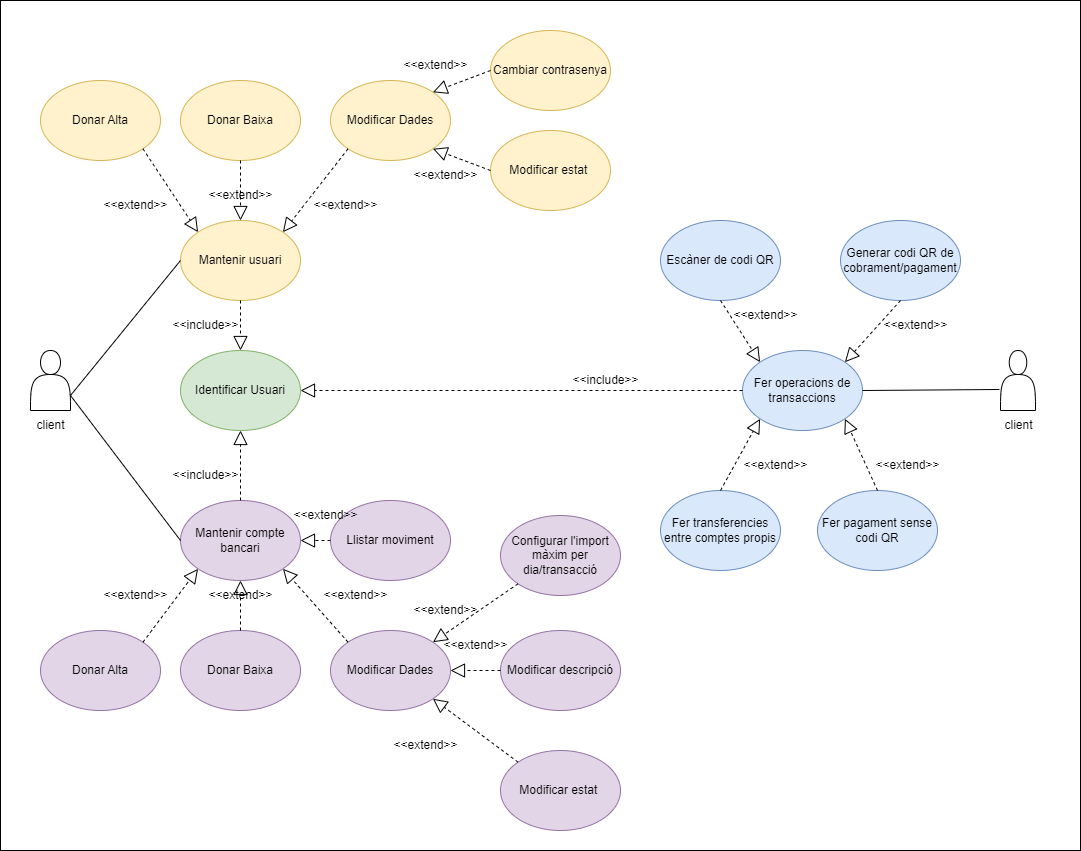
\includegraphics[width=1\textwidth]{imatges/diagrama caso de uso client.png}
    \caption[Diagrama de casos d'ús de context de client.]{Diagrama de casos d'ús de context de client.\pau{``Cambiar'' hauria de ser ``Canviar'', i ``tranferencies'' hauria de ser ``transferències''.} \pau{Si la llegenda és massa llarga i no vols que a l'índex de figures del principi t'hi quedi una frase tan llarga, pots utilitzar els \texttt{[]}, tal com t'ho he posat en aquest cas si mires el codi LaTeX de la figura.}}\sudan{corregit}
    \label{fig:Diagrama de Casos d'Ús de Context de Client}
\end{figure}

\pau{Recorda citar la figura (per exemple: ``El diagrama il·lustrat a la Figura~\ref{fig:Diagrama de Casos d'Ús de Context de Client} mostra les diferents operacions...'').}\sudan{corregit}



L'actor client pot realitzar operacions relacionades amb la gestió del seu compte d'usuari, incloent-hi donar-se d'alta, donar-se de baixa, modificar les seves dades personals, canviar la contrasenya i modificar l'estat del seu compte. Totes aquestes operacions formen part d'un cas d'ús més general anomenat \textbf{Mantenir usuari}, que centralitza aquestes funcions. Per poder realitzar aquestes accions, el client ha de passar pel procés d'\textbf{Identificar usuari}, que és un pas previ necessari per garantir la seguretat de les operacions.\\

A més de gestionar el compte d'usuari, el client també pot gestionar el seu compte bancari a través del cas d'ús \textbf{Mantenir compte bancari}, que inclou accions com donar d'alta un compte, donar-lo de baixa, modificar les dades del compte, llistar els moviments bancaris, i configurar l'import màxim per transacció o per dia. Aquestes funcions estan dissenyades per permetre al client controlar i supervisar les seves operacions bancàries dins del sistema.\\

Un altre grup important de casos d'ús està relacionat amb les \textbf{operacions de transaccions}. Aquí, el client pot escanejar codis QR per realitzar pagaments o cobraments, generar codis QR, fer transferències entre els seus propis comptes i realitzar pagaments sense necessitat d'utilitzar un codi QR. Aquestes operacions són essencials per a la funcionalitat de qualsevol sistema que impliqui gestió financera, ja que permeten al client executar transaccions de manera ràpida i segura.\\



\subsection{Diagrama de casos d'ús de l'usuari administrador}
\label{subsec: Diagrama de casos d'ús de l'usuari administrador}

Aquest segon diagrama de cas d'ús~\ref{subsec: Diagrama de casos d'ús de l'usuari administrador} mostra les diferents funcions que un \textbf{administrador} pot dur a terme dins d'un sistema. L'actor principal és l'administrador, qui interactua amb diversos casos d'ús que representen les operacions disponibles.

\clearpage
\begin{figure}[h]
    \centering
    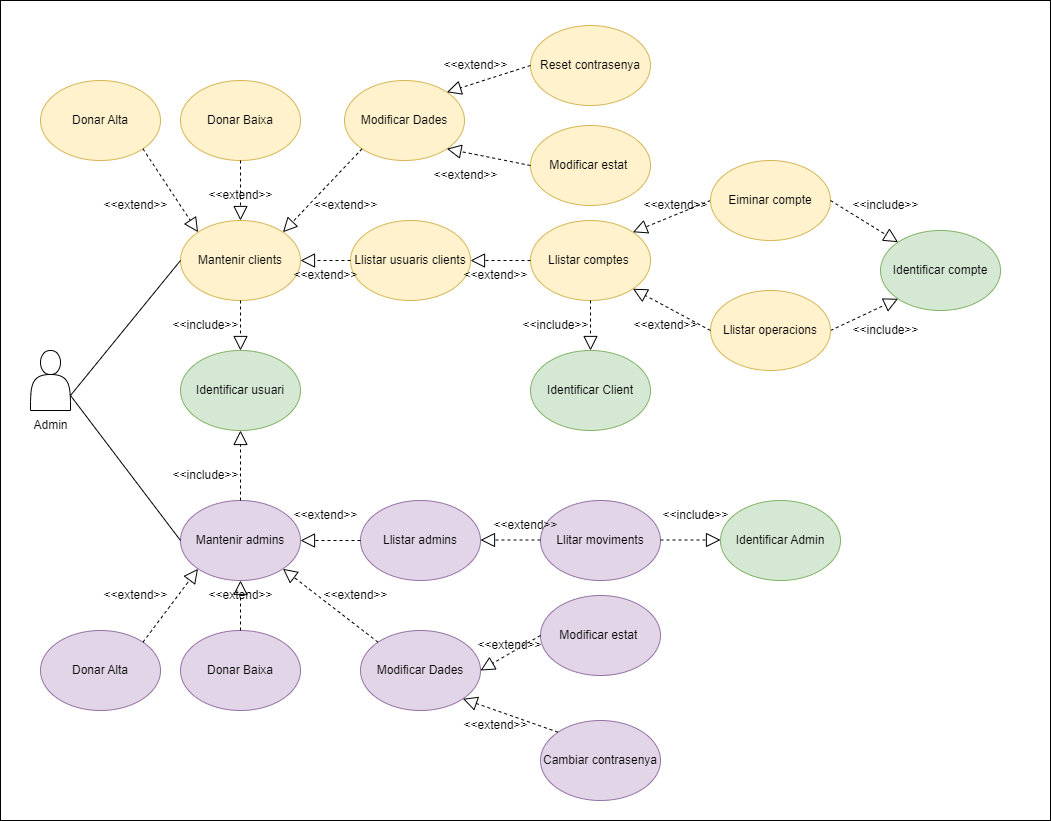
\includegraphics[width=0.9\textwidth]{imatges/diagrama caso de uso admin.png}
    \caption{Diagrama de casos d'ús de context d'administrador. \pau{``Llitar'' hauria de ser ``Llistar'', i ``Cambiar'' hauria de ser ``Canviar''.}}\sudan{corregit}
    \label{fig:Diagrama de Casos d'Ús de Context d'Administrador}
\end{figure}

\pau{Cal citar bé la figura.}\sudan{corregit}


 Un dels casos d'ús centrals és \textbf{Mantenir clients}, que inclou accions com donar d'alta nous clients, donar de baixa clients existents, modificar les dades dels clients, llistar els usuaris clients, restablir la contrasenya dels clients i modificar l'estat dels clients. Un altre cas d'ús important és \textbf{Mantenir admins}, que implica afegir nous administradors, eliminar administradors, modificar les dades dels administradors, llistar els administradors existents i modificar l'estat dels administradors.\\

A més, el diagrama mostra altres casos d'ús relacionats amb la gestió de comptes i operacions. \textbf{Llistar comptes} permet veure la llista de comptes de clients, mentre que \textbf{Eliminar compte} s'encarrega d'eliminar un compte de client. \textbf{Llistar operacions} permet revisar les operacions realitzades pels clients, i \textbf{Llistar moviments} té una funció similar però aplicada als comptes o administradors. També hi ha casos d'ús que fan referència a la identificació d'usuaris, comptes, clients i administradors, mostrant la interrelació entre aquestes operacions i la necessitat d'autenticació o identificació per dur-les a terme.

\subsection{Diagrama de casos d'ús del sistema}
\label{subsec: Diagrama de casos d'ús del sistema}

Addicionalment, el sistema compta amb la funció de generar \textit{logs} per a cada operació, tal com es mostra a la figura~\ref{fig:Diagrama de Casos d'Ús de Context del sistema}. Això vol dir que, fins i tot en cas d'eliminació d'un usuari o un compte, l'historial associat es manté sempre guardat. Aquest enfocament assegura la conservació de dades importants per a possibles auditories o revisions posteriors, garantint així la traçabilitat i la seguretat del sistema.


\begin{figure}[h]
    \centering
    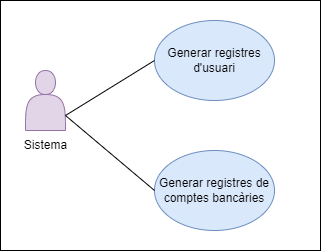
\includegraphics[width=0.6\textwidth]{imatges/logs.png}
    \caption{Diagrama de casos d'ús de context del sistema. \pau{``bancàries'' hauria de ser ``bancaris''.}}\sudan{corregit}
    \label{fig:Diagrama de Casos d'Ús de Context del sistema}
\end{figure}

\pau{Cal citar bé la figura.}\sudan{corregit}



\section{Fitxes de cas d'ús}
\label{sec: fitxes de cas d'ús}

Un fitxer de cas d'ús és un document que descriu detalladament les interaccions entre un usuari i un sistema per aconseguir un objectiu concret. Aquest fitxer és fonamental en el desenvolupament de sistemes informàtics, ja que proporciona una visió clara i comprensible dels requisits funcionals del sistema des de la perspectiva de l'usuari.

A continuació, es presenten cinc fitxers de cas d'ús que han estat creats per descriure les funcionalitats clau del sistema:

\subsection{Generar codi QR de cobrament}
\label{subsec:Generar codi QR de cobrament}

Aquest primer fitxer de cas d'ús que mostra la figura~\ref{fig:Generar codi QR de cobrament} descriu el procés que un usuari segueix per generar un codi QR de cobrament. Inclou la identificació de l'usuari, la validació del compte bancari i la generació del codi QR amb les condicions específiques. Com que es tracta d'un cas de cobrament d'import, els missatges en el codi QR no estan xifrats i, a més, aquest codi QR no caduca mai.


\begin{figure}[h]
    \centering
    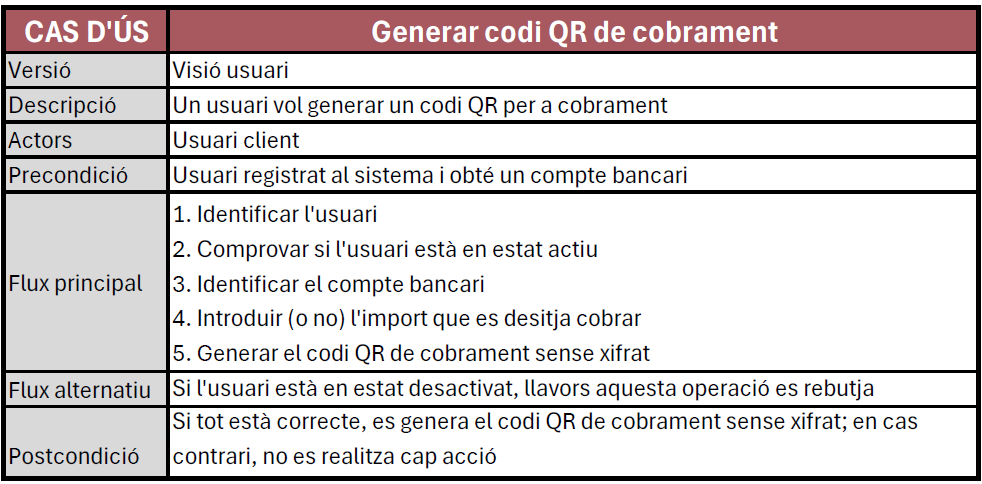
\includegraphics[width=1\textwidth]{imatges/f1.png}
    \caption{Generar codi QR de cobrament}
    \label{fig:Generar codi QR de cobrament}
\end{figure}

\clearpage
\subsection{Generar codi QR de pagament}
\label{subsec:Generar codi QR de pagament}

Aquest segon fitxer de cas d'ús que mostra la figura~\ref{fig:Generar codi QR de pagament} és molt similar al primer. L'única diferència és que, en aquest cas, es tracta d'un pagament, cosa que implica més restriccions. En concret, el missatge del codi QR està xifrat, el codi QR caduca i, a més, un codi QR només pot ser escanejat una sola vegada.



\begin{figure}[h]
    \centering
    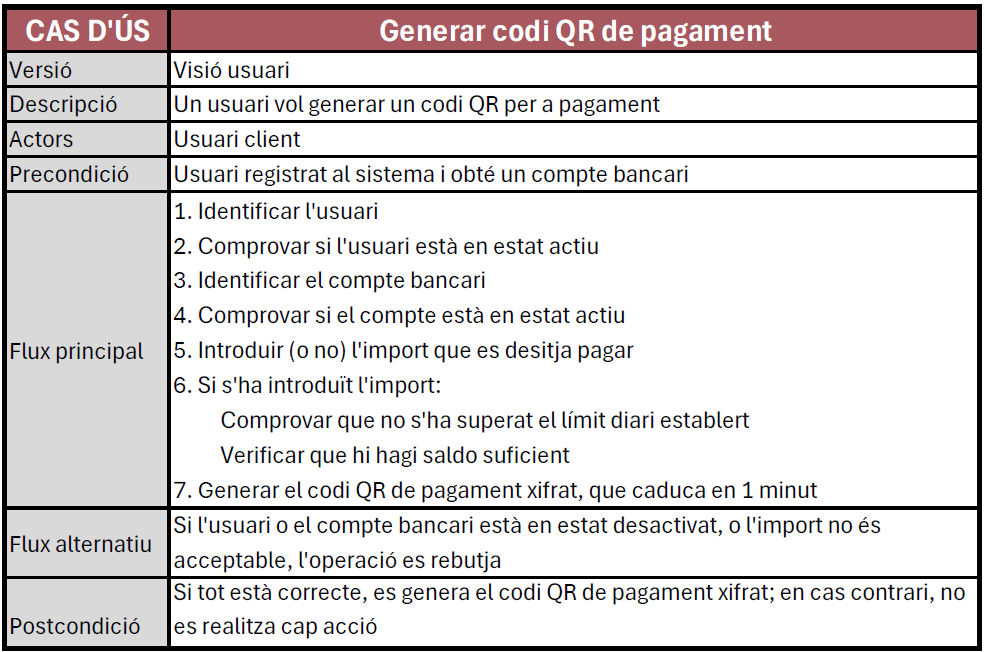
\includegraphics[width=1\textwidth]{imatges/f2.png}
    \caption{Generar codi QR de pagament}
    \label{fig:Generar codi QR de pagament}
\end{figure}

\clearpage


\subsection{Escanejar un codi QR de pagament}
\label{subsec:Escanejar un codi QR de pagament}

El quart fitxer de cas d'ús que mostra la figura~\ref{fig:Escanejar un codi QR de pagament}, detalla els passos que un usuari ha de seguir per escanejar un codi QR de pagament i completar la transacció. Inclou la verificació de l'import i el compte bancari, així com el procés de cobrament.

\begin{figure}[h]
    \centering
    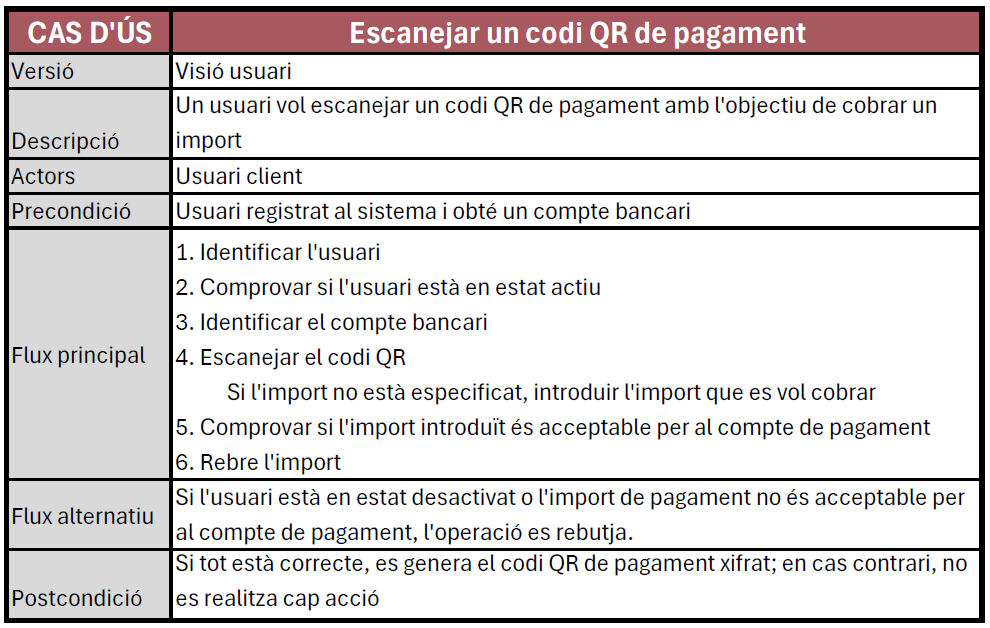
\includegraphics[width=1\textwidth]{imatges/f3.png}
    \caption{Generar codi QR de cobrament}
    \label{fig:Escanejar un codi QR de pagament}
\end{figure}

\clearpage


\subsection{Escanejar un codi QR de cobrament}
\label{subsec:Escanejar un codi QR de cobrament}

Aquest quart fitxer de cas d'ús, que es mostra a la figura~\ref{fig:Escanejar un codi QR de cobrament}, detalla els passos que un usuari ha de seguir per escanejar un codi QR de cobrament i completar la transacció. Inclou la verificació de l’import i el compte bancari, així com el procés de cobrament.

\begin{figure}[h]
    \centering
    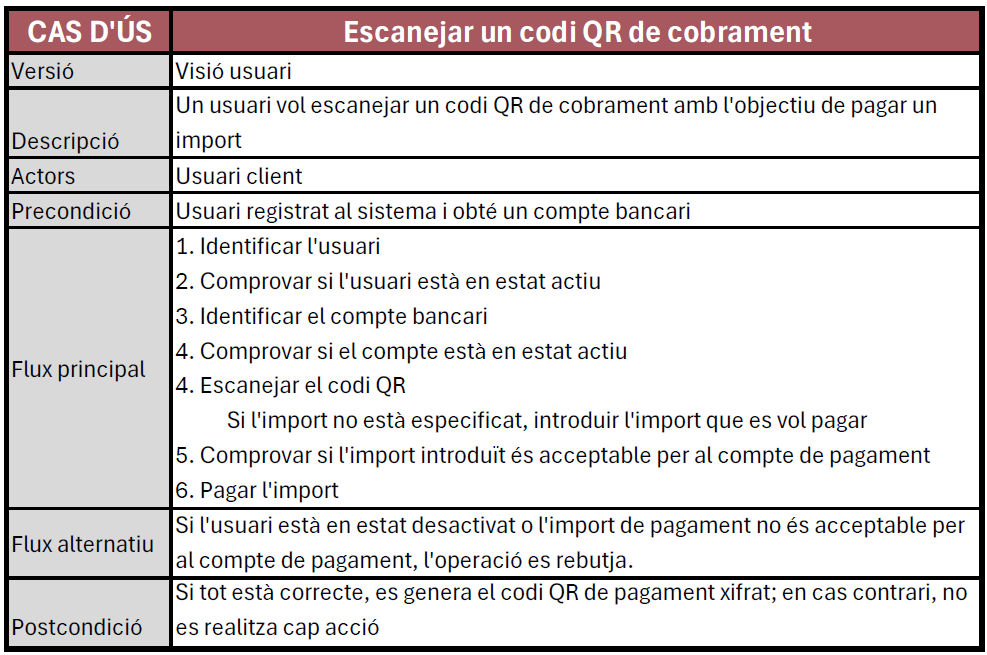
\includegraphics[width=1\textwidth]{imatges/f4.png}
    \caption{Escanejar un codi QR de cobrament}
    \label{fig:Escanejar un codi QR de cobrament}
\end{figure}


\clearpage
\subsection{Modificar l'estat d'un compte bancari}
\label{subsec:Modificar l'estat d'un compte bancari}

El últim fitxer de cas d'ús que apareix a sota de la figura~\ref{fig:Modificar l'estat d'un compte bancari} explica el procés mitjançant el qual un administrador pot canviar l'estat d'un compte bancari associat a un client. Inclou la identificació del compte bancari, la selecció del compte a modificar, i la realització de la modificació.

\begin{figure}[h]
    \centering
    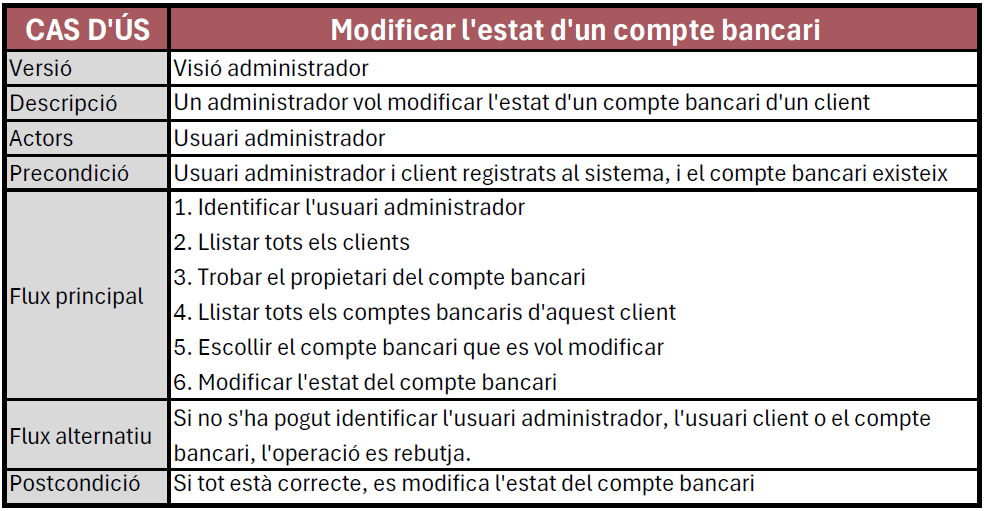
\includegraphics[width=1\textwidth]{imatges/f5.png}
    \caption{Modificar l'estat d'un compte bancari}
    \label{fig:Modificar l'estat d'un compte bancari}
\end{figure}


\pau{Hauries de posar algunes fitxes de cas d'ús. Almenys unes 5 o 6 dels casos d'ús més importants.}

\clearpage
\section{Diagrama de la base de dades}
\label{sec: diagrama de base de dades}

Un diagrama de la base de dades que hi ha a sota és una representació visual que mostra com es distribueixen i organitzen les dades dins d'una base de dades. Aquest tipus de diagrama facilita la comprensió de l'estructura, les relacions i l'organització de les dades dins del sistema. A continuació, es presenta el diagrama~\ref{fig: Diagrama de base de dades} amb una descripció detallada de les seves components principals:


\begin{figure}[h]
    \centering
    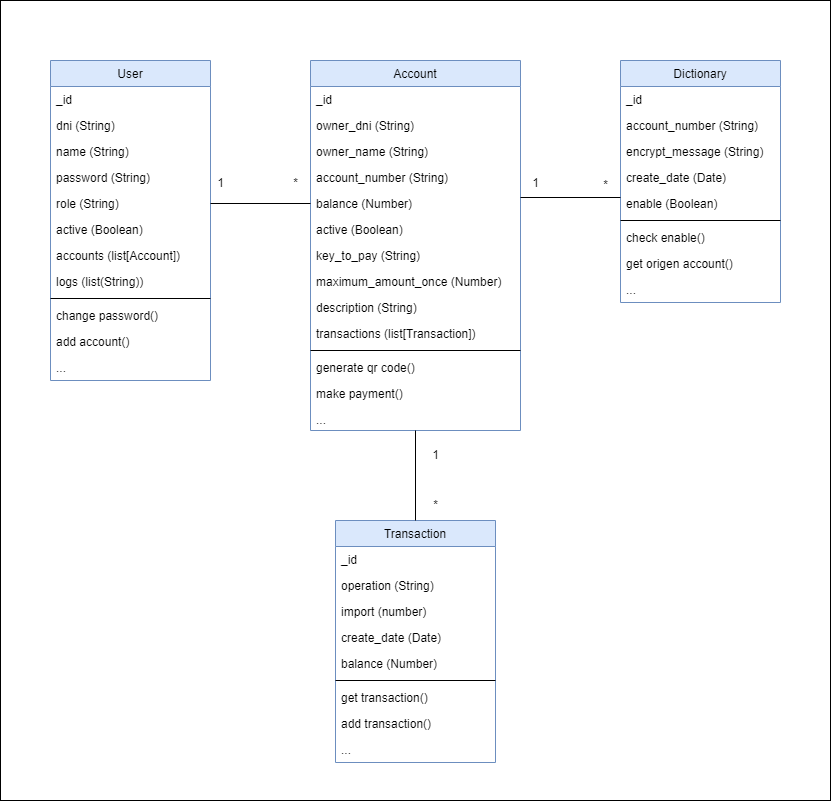
\includegraphics[width=1\textwidth]{imatges/diagrama base dades.png}
    \caption{Diagrama de la base de dades}
    \label{fig: Diagrama de base de dades}
\end{figure}

\pau{Cal citar bé la figura.}\sudan{corregit}

El diagrama representa un model de dades que inclou quatre entitats principals: User, Account, Transaction i Dictionary. Aquestes entitats estan interrelacionades per gestionar informació d'usuaris, comptes, transaccions i altres dades associades.

\subsection{User}
\label{subsec: User}


L'entitat \textbf{User} defineix els usuaris del sistema amb atributs bàsics com el DNI, el nom, la contrasenya, el rol dins del sistema (administrador o client), així com altres camps com l'estat actiu, la llista de comptes associats i els registres d'activitat (\textit{logs}). Aquesta entitat ofereix funcionalitats per canviar la contrasenya, afegir comptes nous i altres operacions relacionades amb l'usuari.\\

Aquesta entitat conté les dades obligatòries que cada usuari ha de tenir:

\begin{itemize}
    \item \textbf{\_id} (Object\_id) [Clau primària]: Generat automàticament per MongoDB.
    \item \textbf{dni} (String) [NOT NULL]: Emmagatzema el número d'identificació de l'usuari, no repetible.
    \item \textbf{name} (String) [NOT NULL]: Emmagatzema el nom de l'usuari.
    \item \textbf{password} (String) [NOT NULL]: Emmagatzema la contrasenya de l'usuari, que s'encripta abans d'inserir-la.
    \item \textbf{role} (String) [NOT NULL]: Emmagatzema el rol de l'usuari, que pot ser administrador o client.
    \item \textbf{active} (Boolean) [DEFAULT: ``true'']: Indica si l'usuari està disponible per fer operacions de transacció.
    \item \textbf{accounts} (Account List) [DEFAULT: []]: Emmagatzema tots els ID de comptes que pertanyen a l'usuari.
    \item \textbf{logs} (String List) [DEFAULT: []]: Emmagatzema els moviments de l'usuari.
\end{itemize}


\subsection{Account}
\label{subsec: Account}


L'entitat \textbf{Account} representa els comptes bancaris associats als usuaris. Cada compte té atributs per identificar el propietari, el saldo disponible, una clau per generar codis QR de pagament, límits de transacció, i una descripció del compte. Els comptes poden generar codis QR per facilitar pagaments o cobraments i tenen associades llistes de transaccions.\\

Cada vegada que es genera un codi QR de pagament, la clau s'actualitza i es guarda la informació necessària a la taula \textbf{Dictionary}. Quan un client escaneja el codi QR, a partir de la taula Dictionary es pot identificar el propietari i obtenir la clau per desxifrar el missatge.\\

Aquesta entitat conté les dades obligatòries que cada compte ha de tenir:

\begin{itemize}
    \item \textbf{\_id} (Object\_id) [Clau primària]: Generat automàticament per MongoDB.
    \item \textbf{owner\_dni} (String) [NOT NULL]: Emmagatzema el DNI del propietari del compte.
    \item \textbf{owner\_name} (String) [NOT NULL]: Emmagatzema el nom del propietari del compte.
    \item \textbf{account\_number} (String) [NOT NULL]: Emmagatzema el número de compte, que ha de ser únic.
    \item \textbf{balance} (Number) [NOT NULL]: Emmagatzema el saldo disponible en el compte.
    \item \textbf{active} (Boolean) [DEFAULT: ``true'']: Indica si el compte està actiu i pot realitzar transaccions.
    \item \textbf{key\_to\_pay} (String) [NOT NULL]: Emmagatzema una clau per generar codis QR de pagament.
    \item \textbf{maximum\_amount\_once} (Number) [DEFAULT: 0]: Indica la quantitat màxima que es pot pagar en una sola transacció.
    \item \textbf{description} (String) [OPTIONAL]: Conté una descripció addicional del compte.
    \item \textbf{transactions} (Transaction List) [DEFAULT: []]: Emmagatzema la llista de transaccions associades al compte.
\end{itemize}


\clearpage


\subsection{Dictionary}
\label{subsec: Dictionary}

L'entitat \textbf{Dictionary} que mostra la figura~\ref{fig: Ús de Dictionary} de sota emmagatzema informació complementària relacionada amb els comptes i les transaccions. Aquesta entitat es fa servir per guardar dades com missatges encriptats, dates de creació, i estats d'activació, permetent verificar i processar correctament les operacions financeres dins del sistema.\\


\begin{figure}[h]
    \centering
    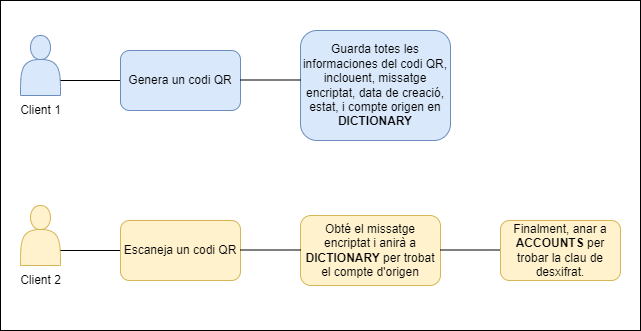
\includegraphics[width=1\textwidth]{imatges/dictionary.png}
    \caption{Ús de Dictionary. \pau{Canviar ``informaciones'' per ``informacions'', ``inclouent, missatge'' per ``incloent missatge'', ``en DICTIONARY'' per ``a la taula Dictionary'', ``a DICTIONARY per trobat'' per ``a la taula Dictionary per trobar'', i ``a ACCOUNTS'' per ``a la taula Account''.}}\sudan{corregit}
    \label{fig: Ús de Dictionary}
\end{figure}



\pau{Cal citar bé la figura.}

Aquesta entitat conté les dades obligatòries que cada entrada ha de tenir:

\begin{itemize}
    \item \textbf{\_id} (Object\_id) [Clau primària]: Generat automàticament per MongoDB.
    \item \textbf{account\_number} (String) [NOT NULL]: Emmagatzema el número de compte associat.
    \item \textbf{encrypt\_message} (String) [NOT NULL]: Conté el missatge encriptat relacionat amb la transacció.
    \item \textbf{create\_date} (Date) [NOT NULL]: Indica la data de creació de l'entrada al diccionari.
    \item \textbf{enable} (Boolean) [DEFAULT: ``true'']: Indica si l'entrada està activa i disponible per ser utilitzada.
\end{itemize}



\subsection{Transaction}
\label{subsec: Transaction}


L'entitat \textbf{Transaction} descriu les operacions financeres realitzades en un compte. Aquesta entitat emmagatzema informació detallada sobre cada transacció, com ara el tipus d'operació, l'import, i el saldo resultant. Cada transacció genera dues instàncies: una per al compte d'origen (qui paga) i una altra per al compte de destí (qui cobra). Aquest diagrama reflecteix com les entitats es connecten per permetre la gestió d'usuaris, comptes i transaccions dins del sistema.\\

Aquesta entitat conté les dades obligatòries que cada transacció ha de tenir:

\begin{itemize}
    \item \textbf{\_id} (Object\_id) [Clau primària]: Generat automàticament per MongoDB.
    \item \textbf{operation} (String) [NOT NULL]: Indica el tipus d'operació realitzada (per exemple, ``pagament'' o ``cobrament'').
    \item \textbf{amount} (Number) [NOT NULL]: Emmagatzema l'import de la transacció.
    \item \textbf{create\_date} (Date) [NOT NULL]: Indica la data de creació de la transacció.
    \item \textbf{balance} (Number) [NOT NULL]: Reflecteix el saldo resultant en el compte després de la transacció.
    \item \textbf{origin\_account} (String) [NOT NULL]: Emmagatzema el número de compte d'origen de la transacció.
    \item \textbf{destination\_account} (String) [NOT NULL]: Emmagatzema el número de compte de destí de la transacció.
\end{itemize}


\section{Diagrama de processos}
\label{ sec: Diagrama de processos }

Aquesta diagrama de flux~\ref{fig: Diagrama de processos} representa els processos de gestió d'usuaris i transaccions de pagament mitjançant codis QR. Mostra com les diferents decisions i funcions es ramifiquen en funció de les característiques i accions de l'usuari, garantint que cada procés es gestiona adequadament segons les condicions del sistema.


\clearpage

\begin{figure}[h]
    \centering
    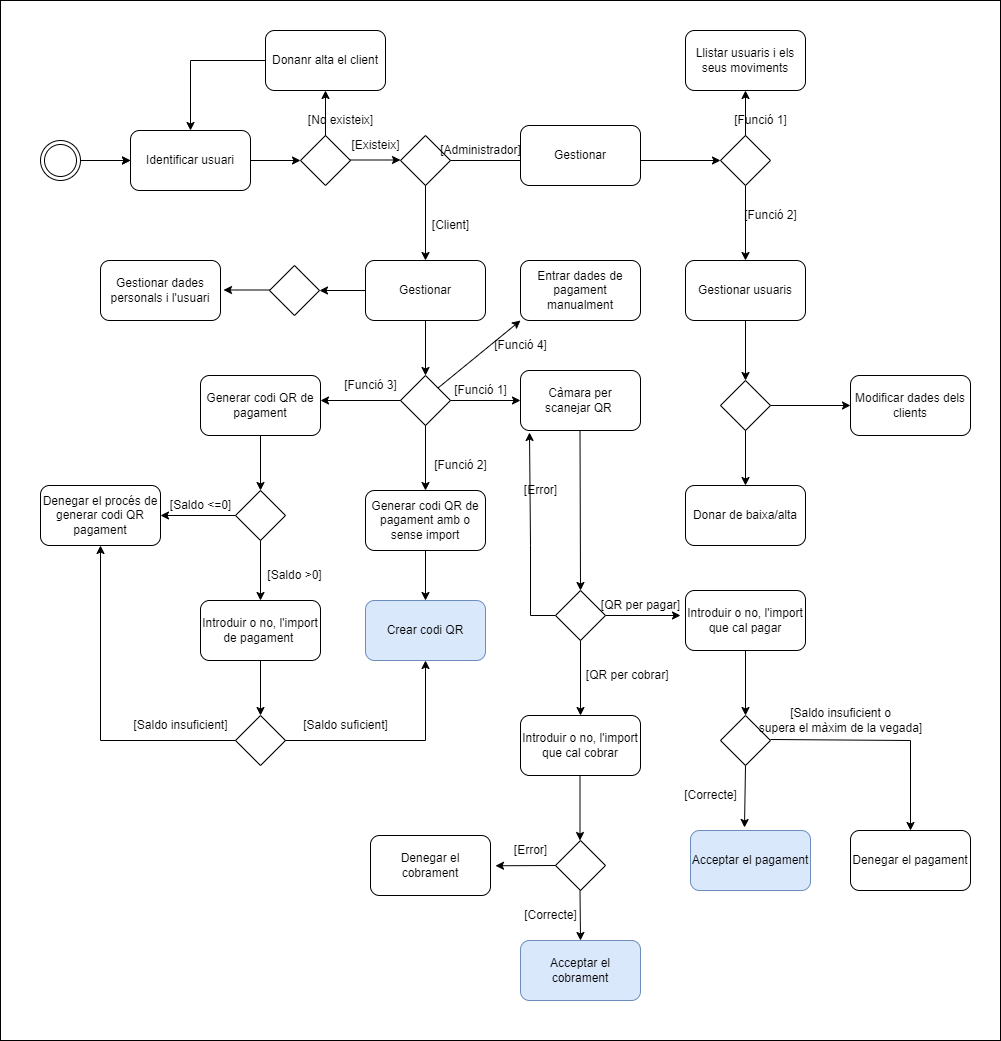
\includegraphics[width=1\textwidth]{imatges/diagrama processos.png}
    \caption{Diagrama de processos.}
    \label{fig: Diagrama de processos}
\end{figure}

\pau{Cal citar bé la figura.}\sudan{corregit}




\subsection{Descripció del procés}
\label{subsec:Descripció del procés}


\begin{itemize}
    \item \textbf{Identificació de l'usuari}: El procés comença amb la identificació de l'usuari. Si l'usuari no existeix, es procedeix a \textbf{donar d'alta el client}. Si l'usuari existeix, es determina si és un \textbf{administrador} o un \textbf{client}.
    
    \item \textbf{Administradors}: 
    \begin{itemize}
        \item \textbf{Funció 1}: Permet \textbf{llistar usuaris i els seus moviments}.
        \item \textbf{Funció 2}: Permet \textbf{gestionar usuaris}, amb accions com \textbf{modificar les dades dels clients} o \textbf{donar-los d'alta o de baixa}.
    \end{itemize}
    
    \item \textbf{Clients}: 
    \begin{itemize}
        \item Si l'usuari és un client, té l'opció de \textbf{gestionar les seves dades personals i d'usuari}.
        \item També pot optar per \textbf{entrar les dades de pagament manualment}, una solució en cas que la càmera no funcioni.
        \item \textbf{Funcions 2 i 3}: S'utilitzen per generar el codi QR de cobrament i de pagament. En cas de cobrament, no cal fixar-se en res \pau{(no cal fixar res, o no cal fixar-se en res?)}\sudan{corregit}, però en cas de pagament, cal verificar si el compte disposa de saldo suficient. Un cop generat el codi QR, la càmera entra en joc per escanejar-lo.
        \item \textbf{Funció 1}: La càmera s'encarrega de llegir el text que hi ha darrere del codi QR i, si el missatge és correcte, processa l'operació.
        \item Cal destacar que es pot introduir l'import tant en el moment de generar el codi QR com després d'escanejar-lo.
    \end{itemize}
\end{itemize}




\section{Interfícies d'usuari}
\label{ sec: Interfícies d'usuari }


El disseny de les interfícies d'usuari ha estat una prioritat abans d'endinsar-nos en el desenvolupament del \textit{front end}. Aquestes interfícies proporcionen una visió preliminar de l'aspecte i la sensació que tindrà l'aplicació. Les figures següents mostren els dissenys de les interfícies d'usuari. \\

Dissenyar tots els possibles estats de l'aplicació en un temps tan limitat és inviable. No obstant això, atès que l'aplicació principal i la dels usuaris comparteixen gran part de la seva interfície, només s'han dissenyat les vistes principals. En desenvolupar l'aplicació de l'usuari, la majoria dels components s'han reutilitzat, modificant-ne el comportament segons les necessitats, ja que les interaccions dels usuaris són limitades.\\

És important destacar que algunes vistes no corresponen exactament a com són a l'aplicació final, principalment perquè s'han modificat o afegit funcionalitats segons les necessitats durant el desenvolupament.\\

\pau{Per cada secció caldria explicar una mica la interfície (quines opcions té, per a què serveix cada botó... una explicació molt senzilla), i citar correctament la figura que s'està descrivint.}


\subsection{Client}
\label{subsec: Client}

L'usuari client és qui utilitza les funcionalitats de l'aplicació per gestionar les seves pròpies operacions i accions.

\subsubsection{Primeres pàgines}
\label{subsubsec: Primeres pàgines}

Al entrar a l'aplicació, es mostra una pàgina de benvinguda. Aquesta pàgina durarà 3 segons, després anirà a la pàgina de \textbf{Login}.\\

En el cas que el client no estigui registrat, cal anar primer a la pàgina de registre per donar-se d'alta. Amb el botó de \textbf{Register} s'anirà a la pàgina de registre.


\begin{figure}[h]
    \centering
    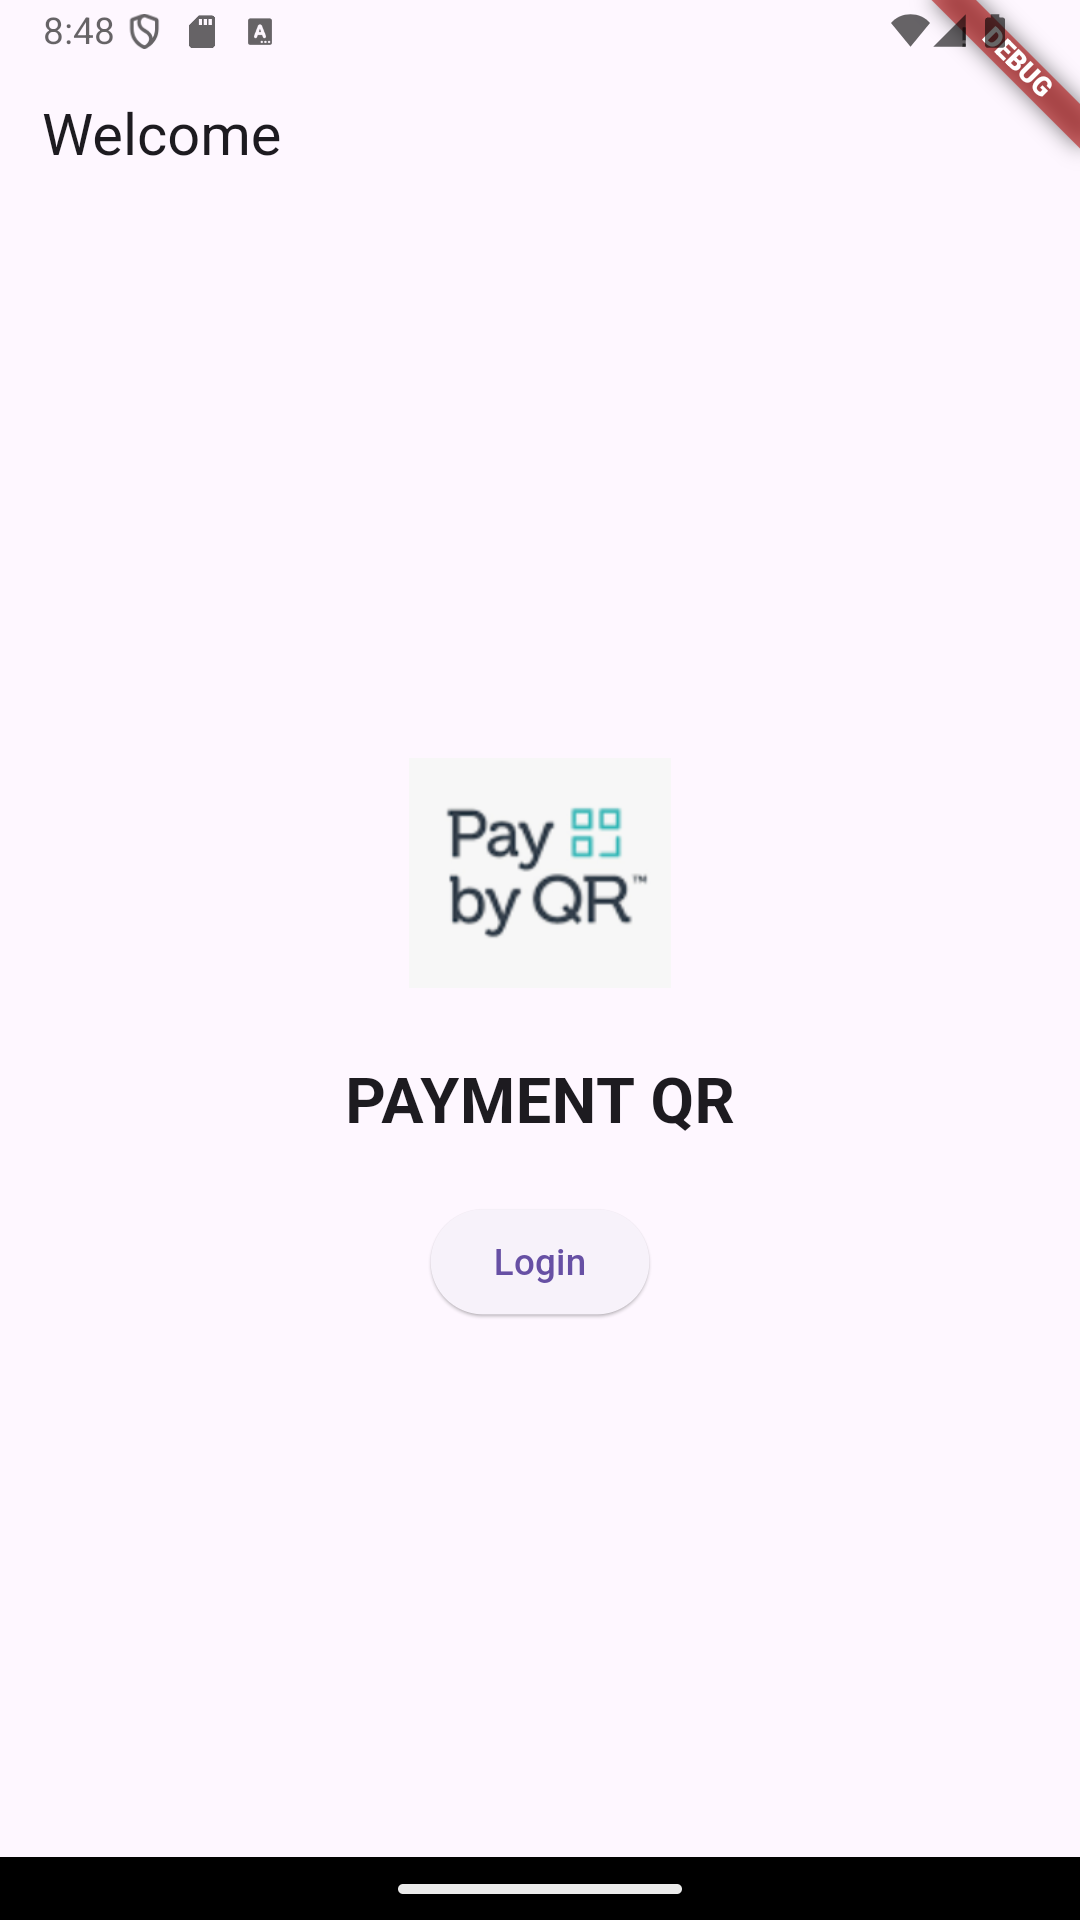
\includegraphics[width=0.4\textwidth]{imatges/welcomepage.png}
    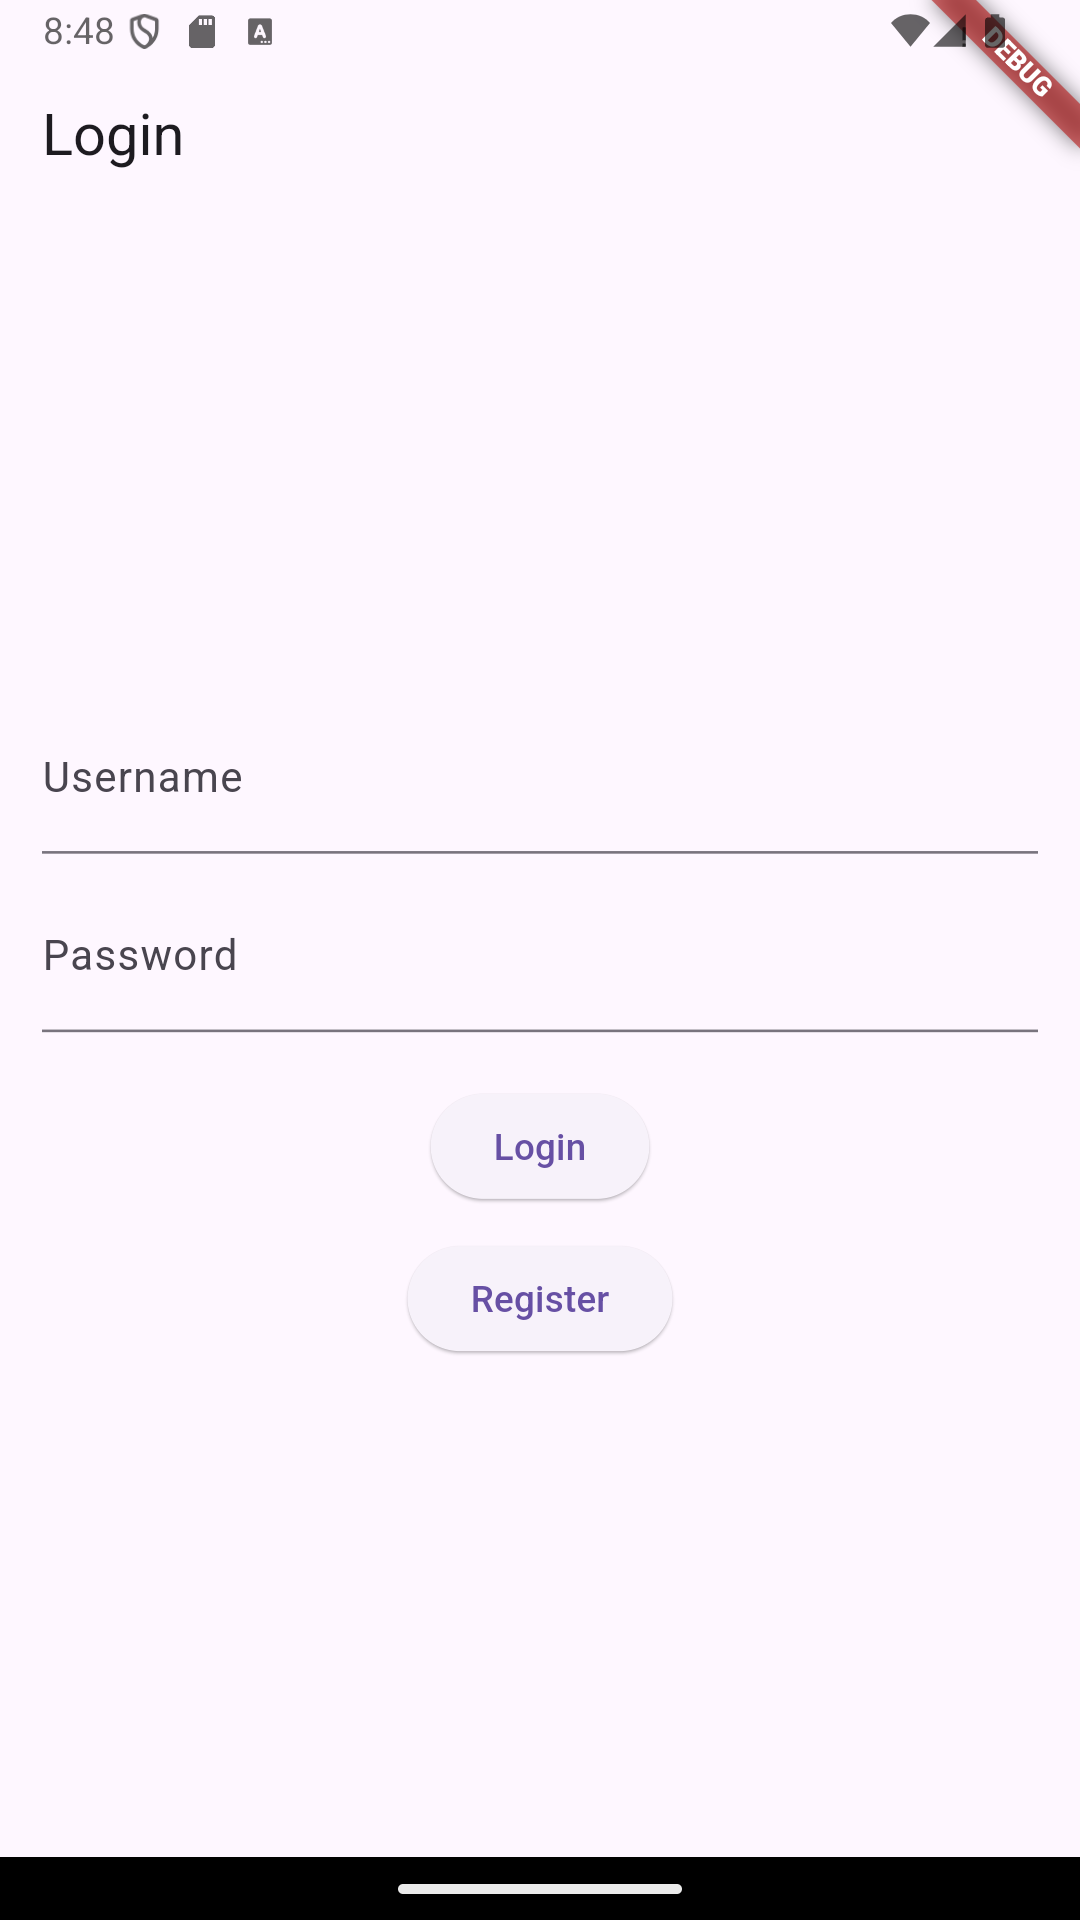
\includegraphics[width=0.4\textwidth]{imatges/login.png}
    \caption{Primeres pàgines}
    \label{fig: Primeres pàgines}
\end{figure}

\clearpage
\subsubsection{Registrar un nou usuari}
\label{subsubsec: Registrar un nou usuari}

El sistema fa una comprovació per verificar si les dades introduïdes corresponen al format esperat.\\

Si les dades són correctes, envia la informació al servidor per iniciar el procés de registre. Si no ho són, el sistema indicarà que no s'ha pogut completar l'operació de registre. Si tot està correcte, s'anirà automàticament a la pàgina de \texttt{login}.

\begin{figure}[h]
    \centering
    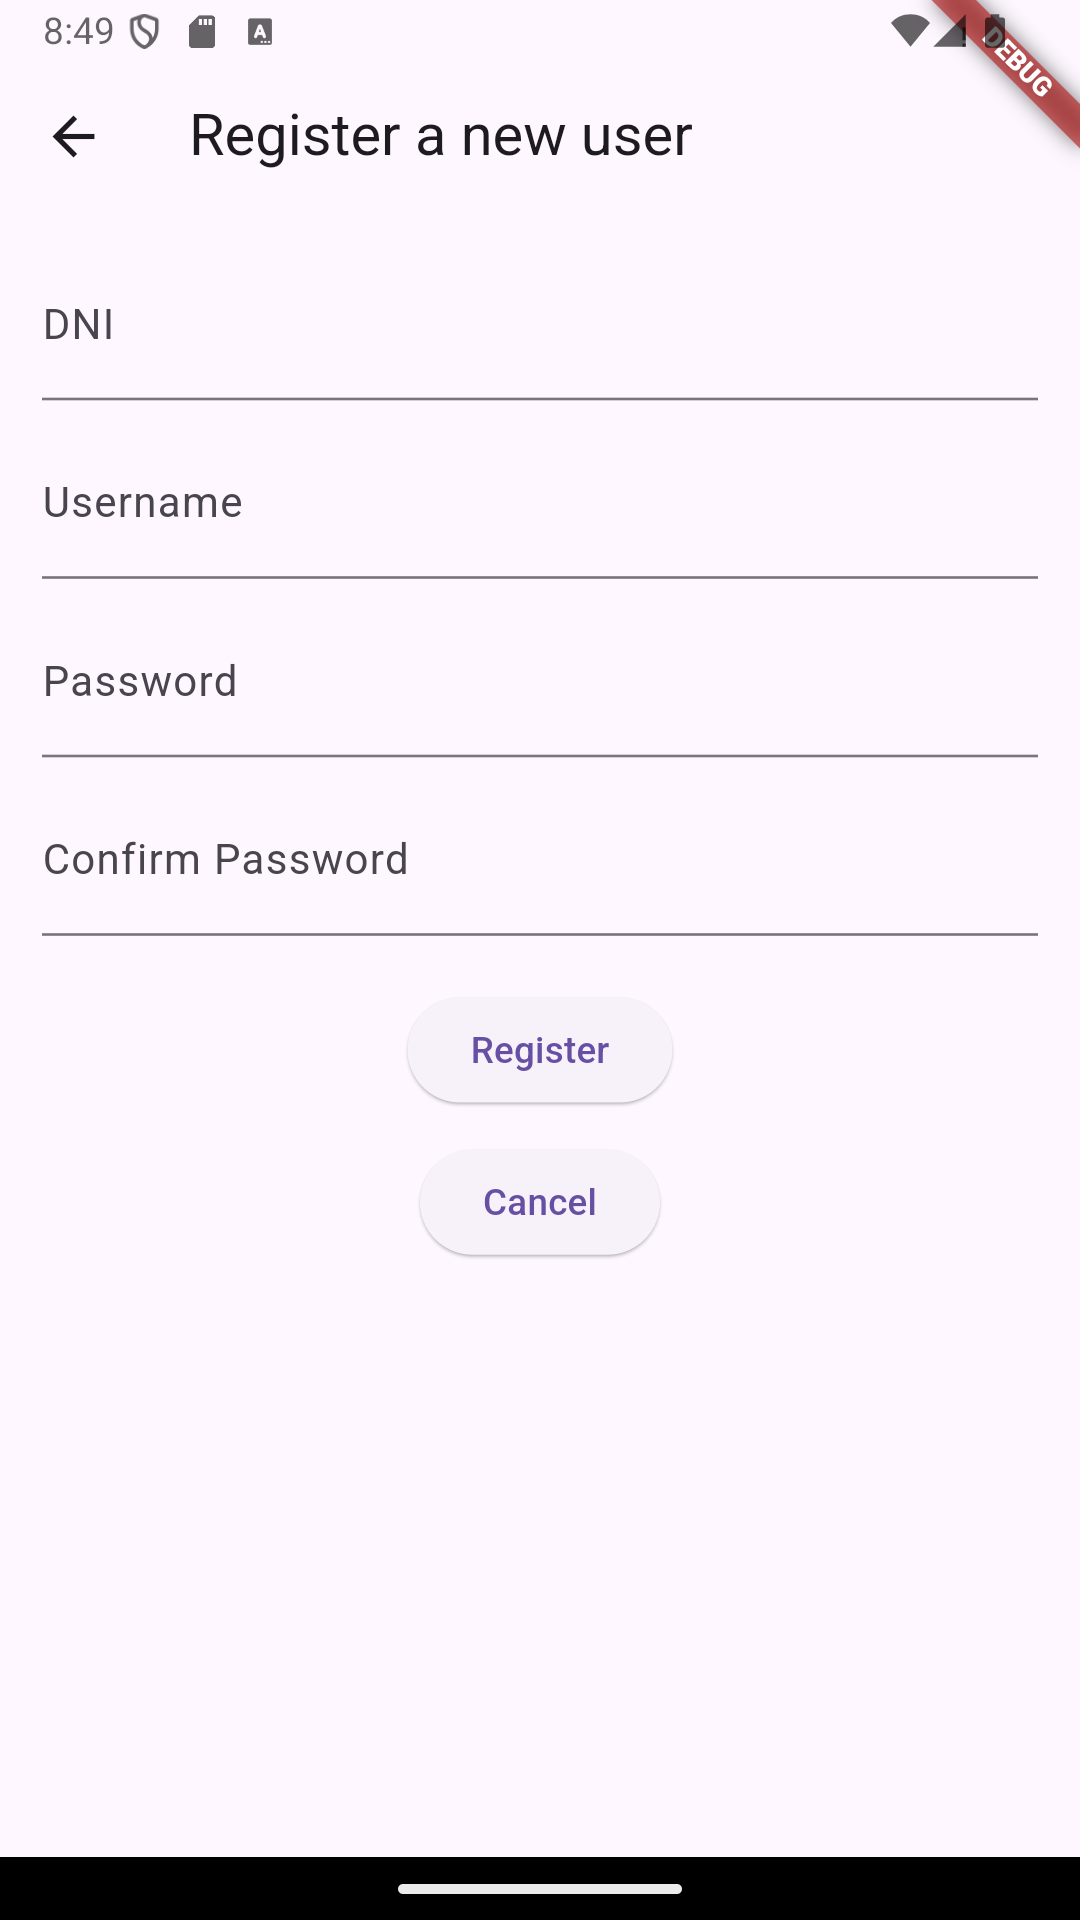
\includegraphics[width=0.4\textwidth]{imatges/registration.png}
    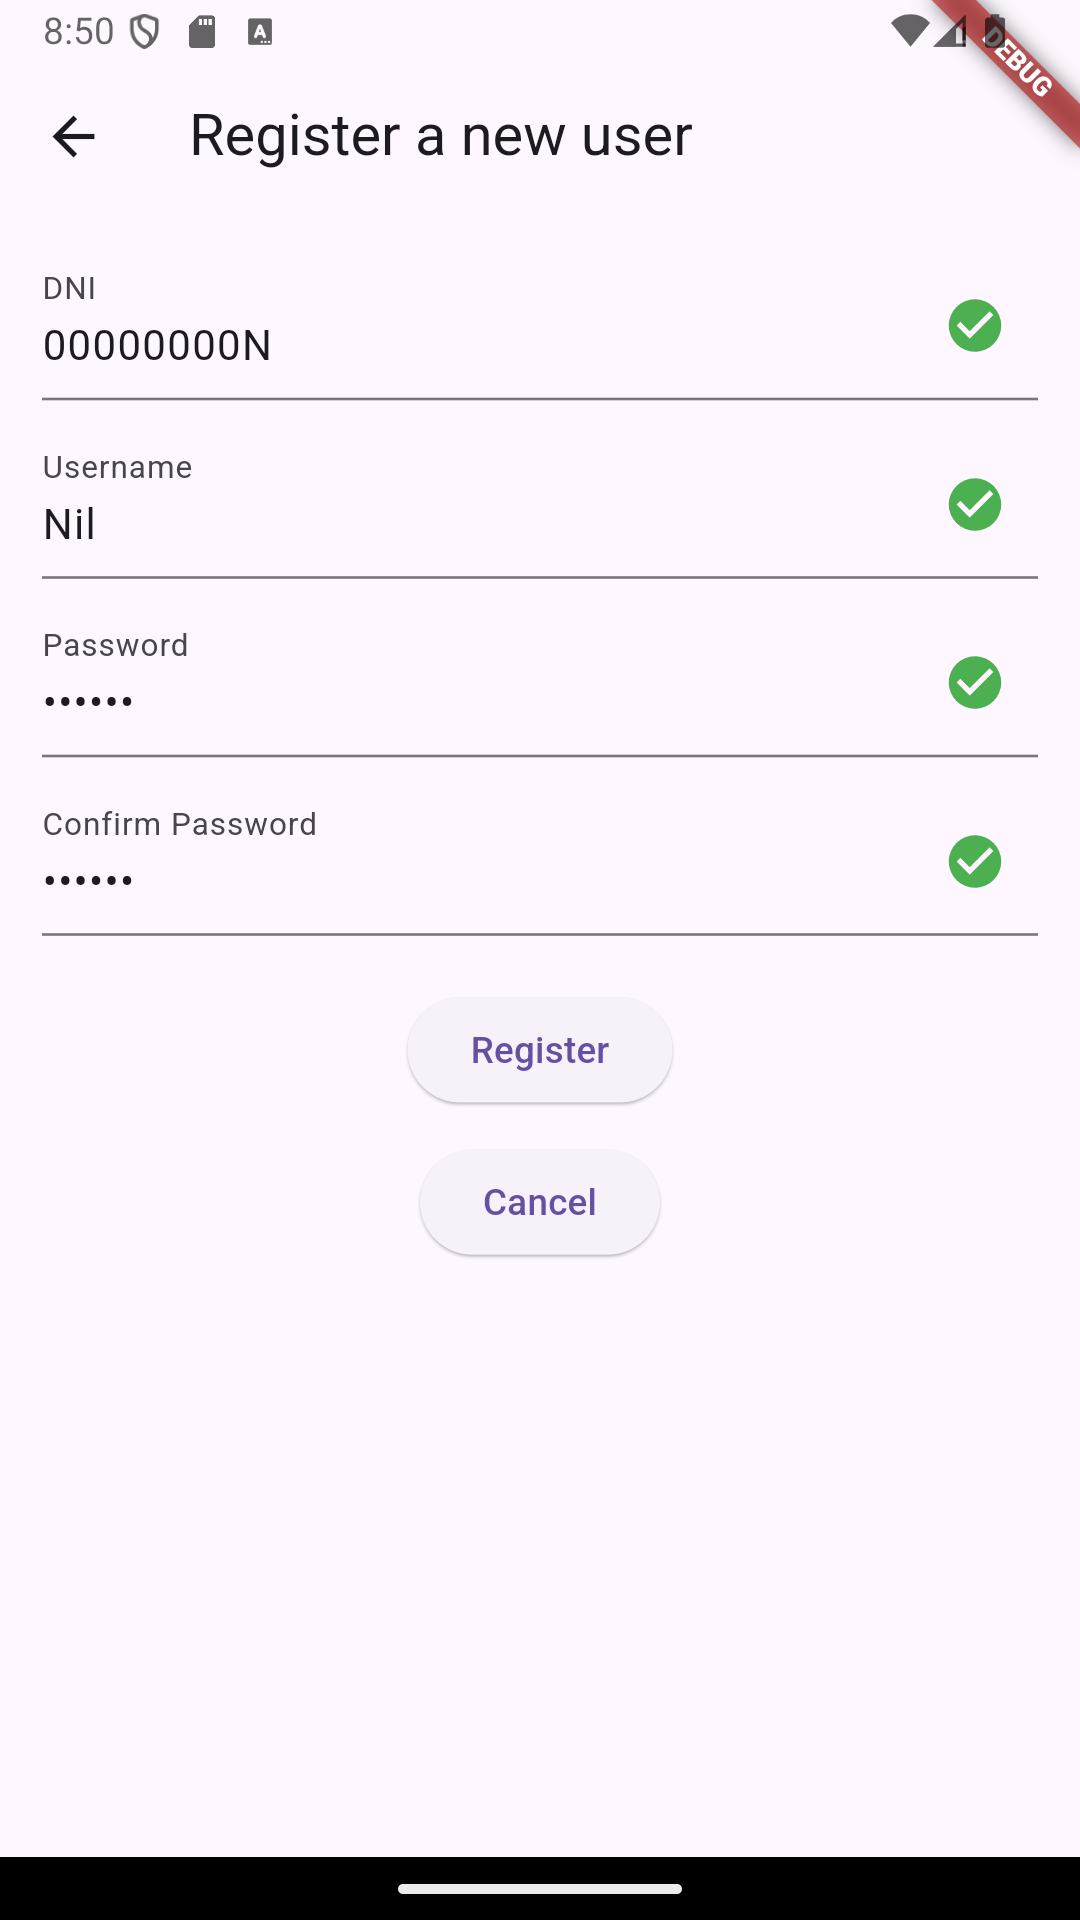
\includegraphics[width=0.4\textwidth]{imatges/registrationwithvalue.png}
    \caption{Registrar nou usuari client}
    \label{fig: registrar nou usuari client}
\end{figure}

\clearpage

\subsubsection{Login}
\label{subsubsec:Login}

Una vegada l'usuari estigui registrat, podrà accedir a l'aplicació. La figura de la dreta mostra la pàgina principal de l'aplicació, on apareixen diversos botons. A les figures següents es detallarà el significat de cadascun d'aquests elements.

\begin{figure}[h]
    \centering
    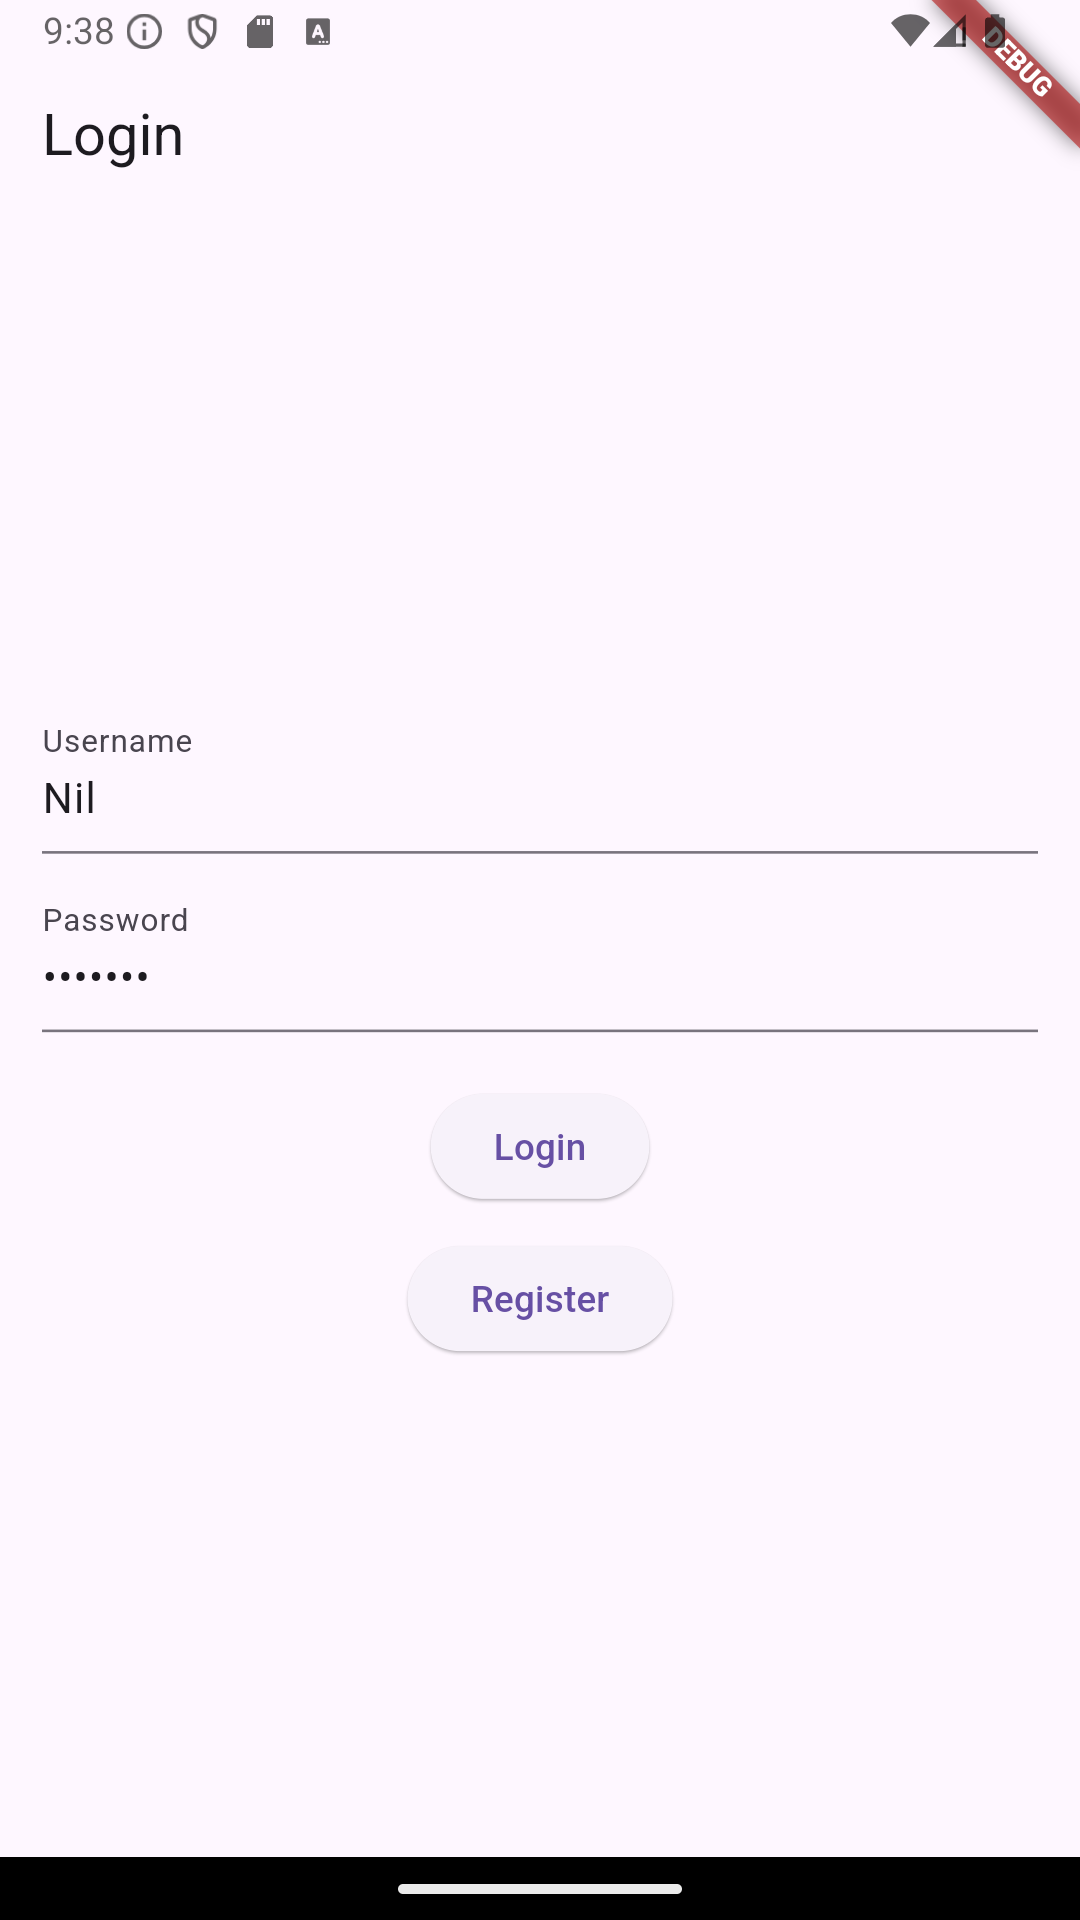
\includegraphics[width=0.4\textwidth]{imatges/loginNil.png}
    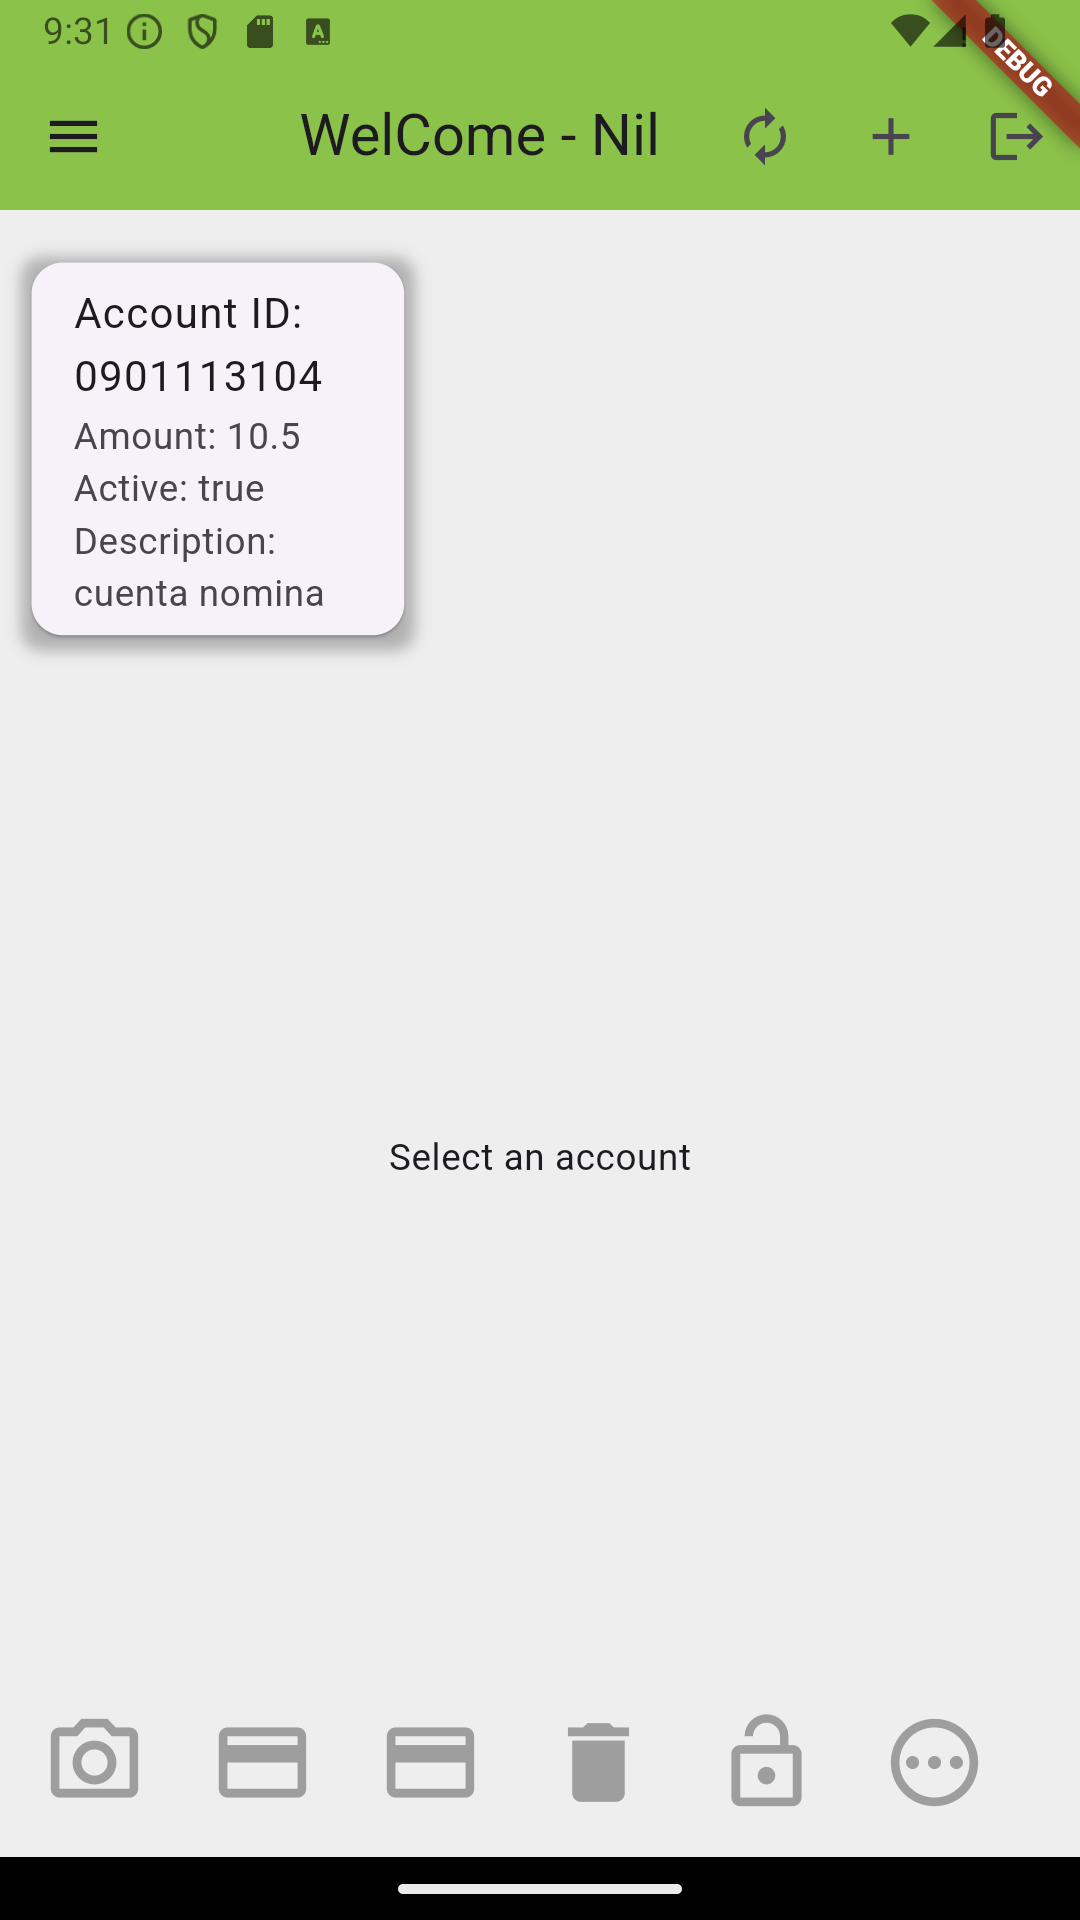
\includegraphics[width=0.4\textwidth]{imatges/mainPage.png}
    \caption{Pàgina de \textit{login} - Client.}
    \label{fig: Pàgina de login - client}
\end{figure}

\clearpage

\subsubsection{Càmera per escanejar codi QR}
\label{subsubsec:Càmera per escanejar codi QR}

Per activar la funció de la càmera, primer cal seleccionar un compte bancari. A continuació, utilitza la càmera per escanejar un codi QR generat prèviament. La càmera escanejarà el codi i, si les dades són correctes, es processarà l'operació. Si tot va bé, es mostrarà un missatge de 'OK' amb els detalls de l'operació, i finalment es proporciona un botó per tornar a la pàgina principal.\\

En tornar a la pàgina principal, es mostrarà la transacció que s'ha fet just abans.

\begin{figure}[h]
    \centering
    % Primera fila de dos imatges
    \begin{minipage}{0.31\textwidth}
        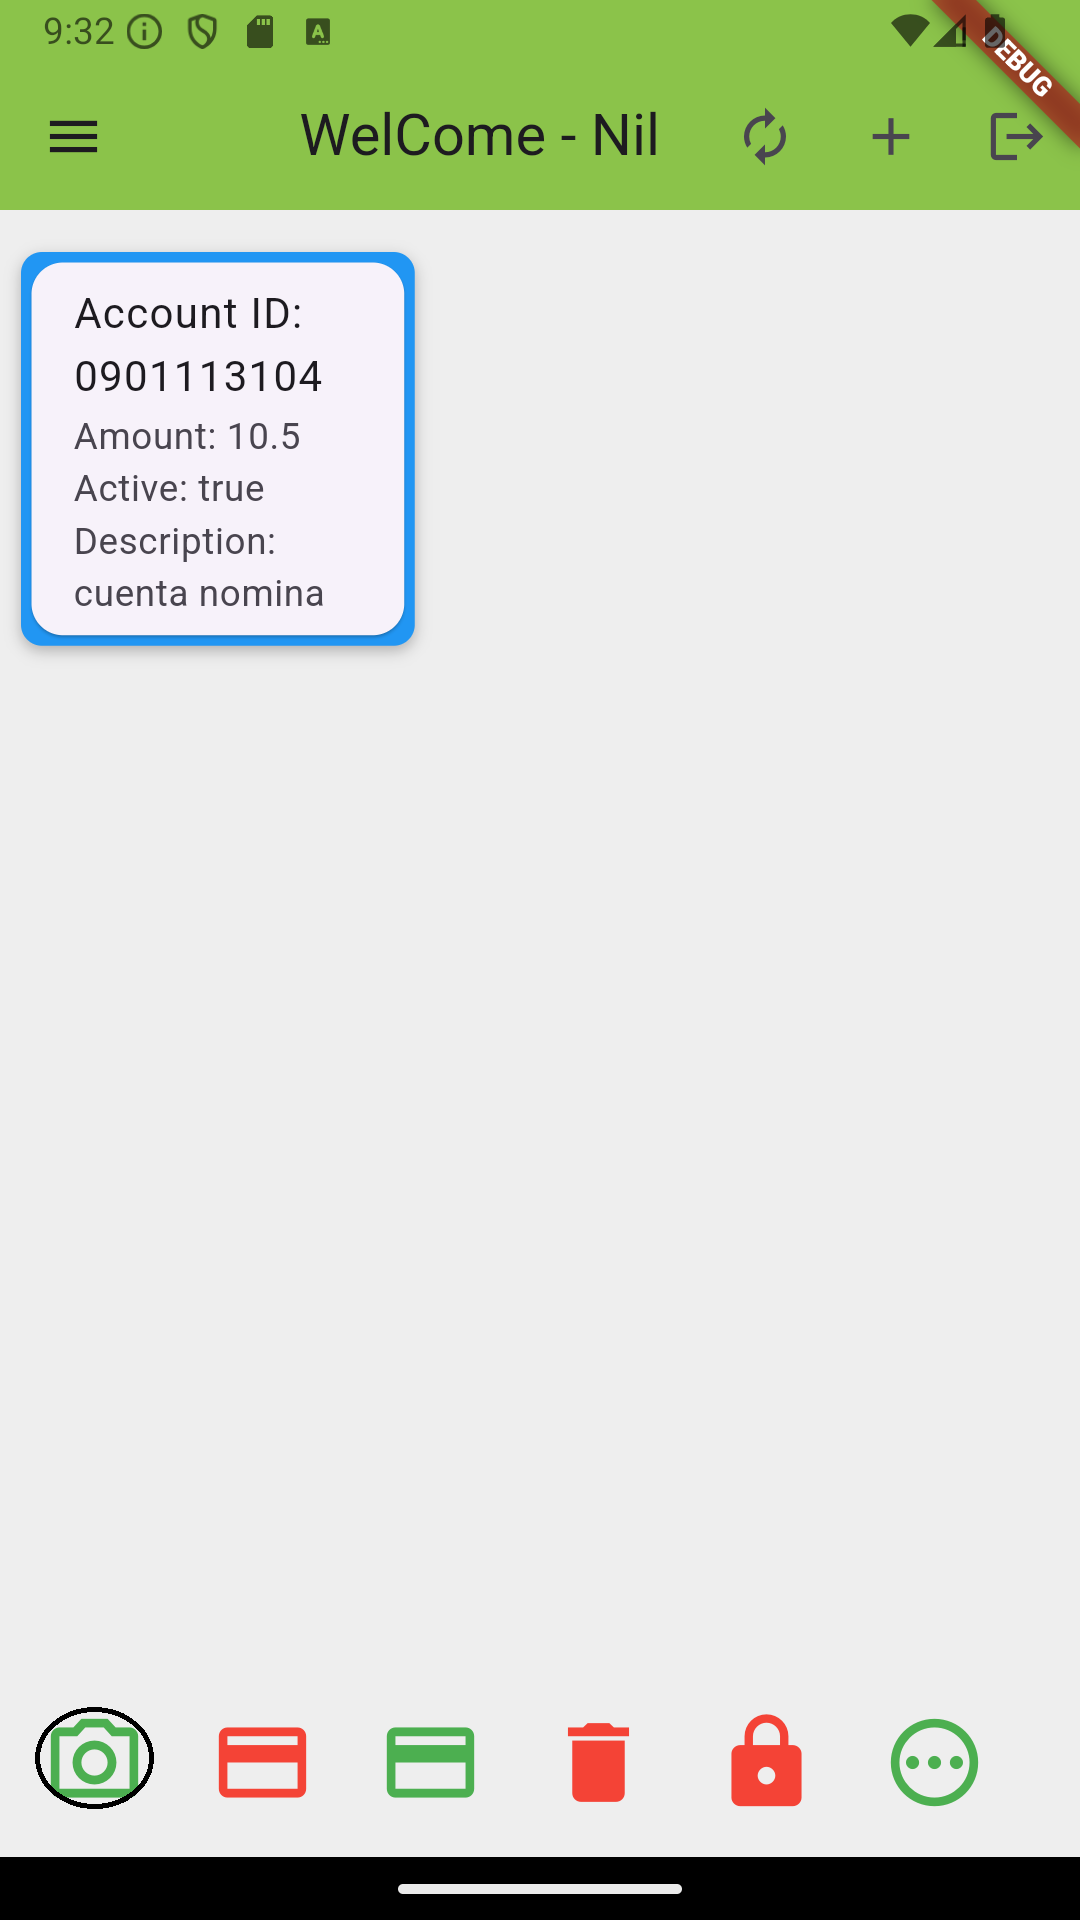
\includegraphics[width=\linewidth]{imatges/mainpageAccount1.png}
        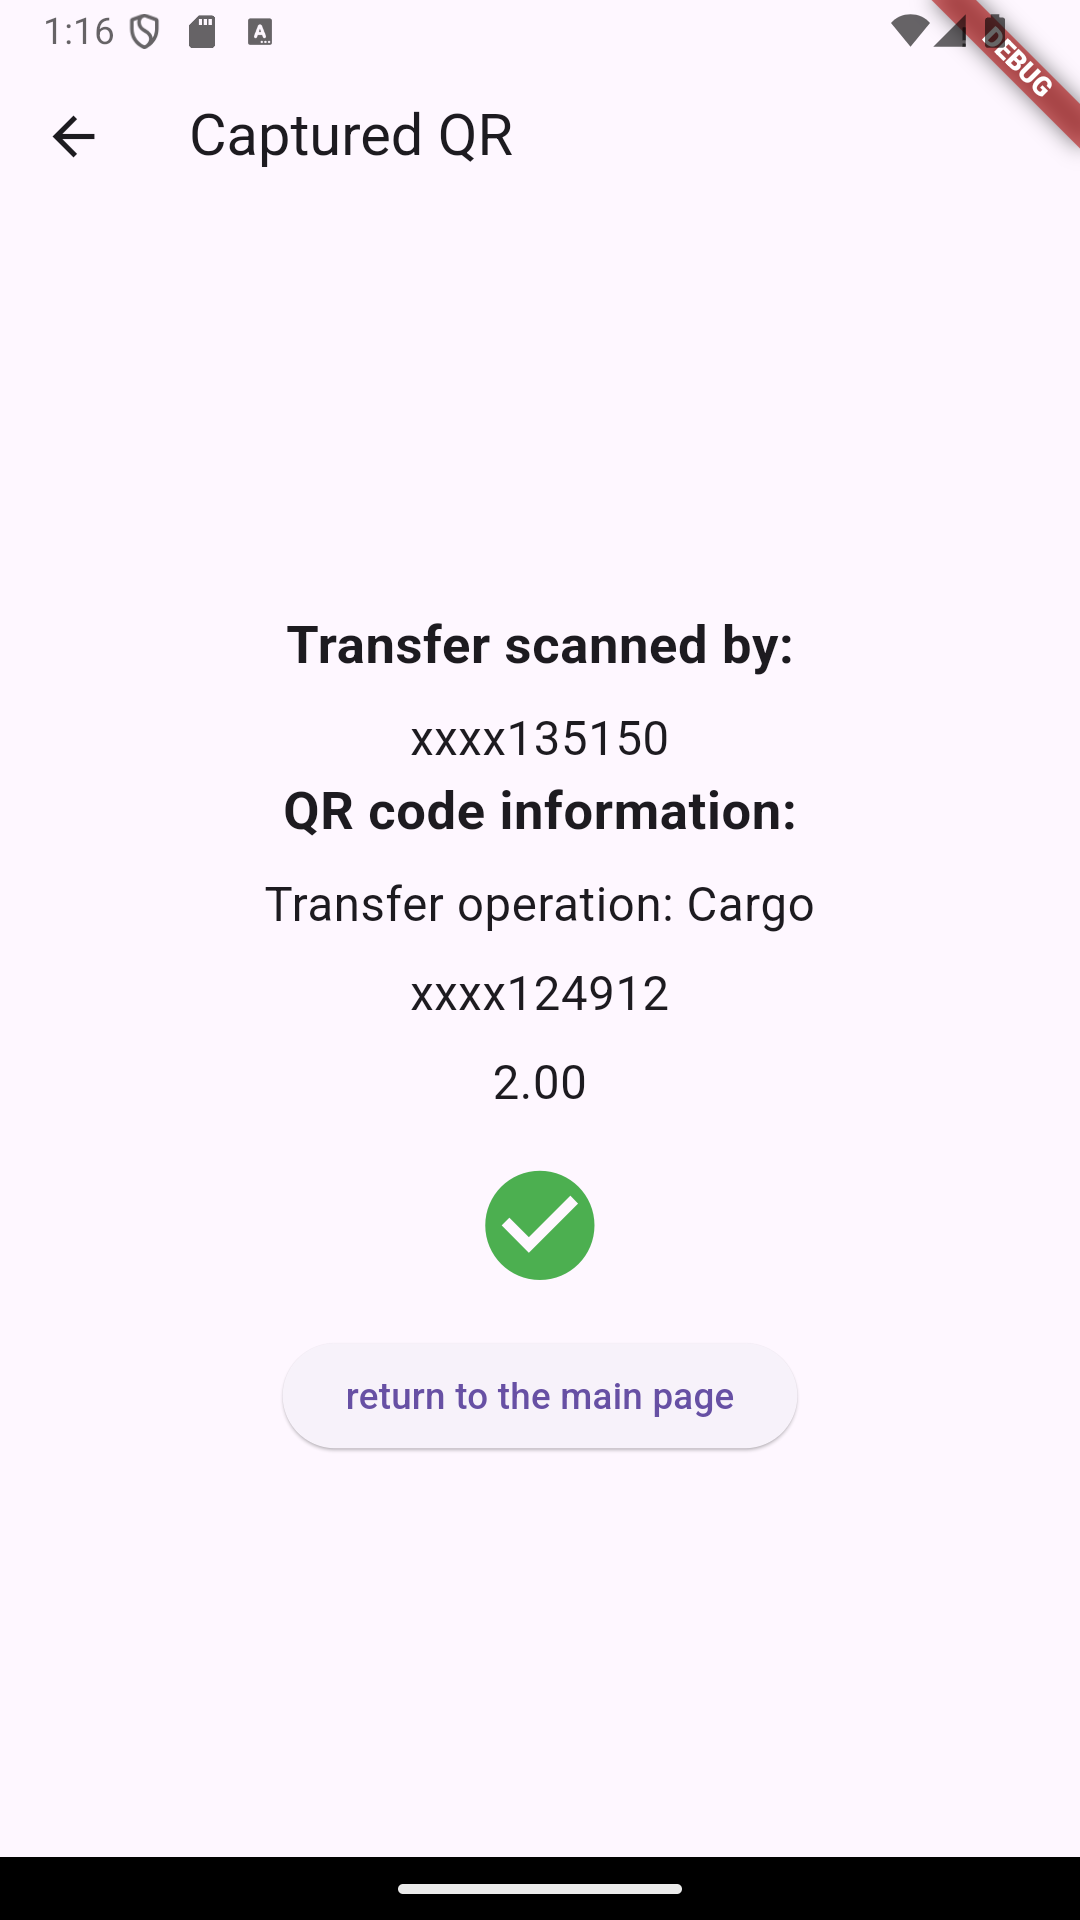
\includegraphics[width=\linewidth]{imatges/capturedQR.png}
    \end{minipage}
    % Segona fila de tres imatges
    \begin{minipage}{0.31\textwidth}
        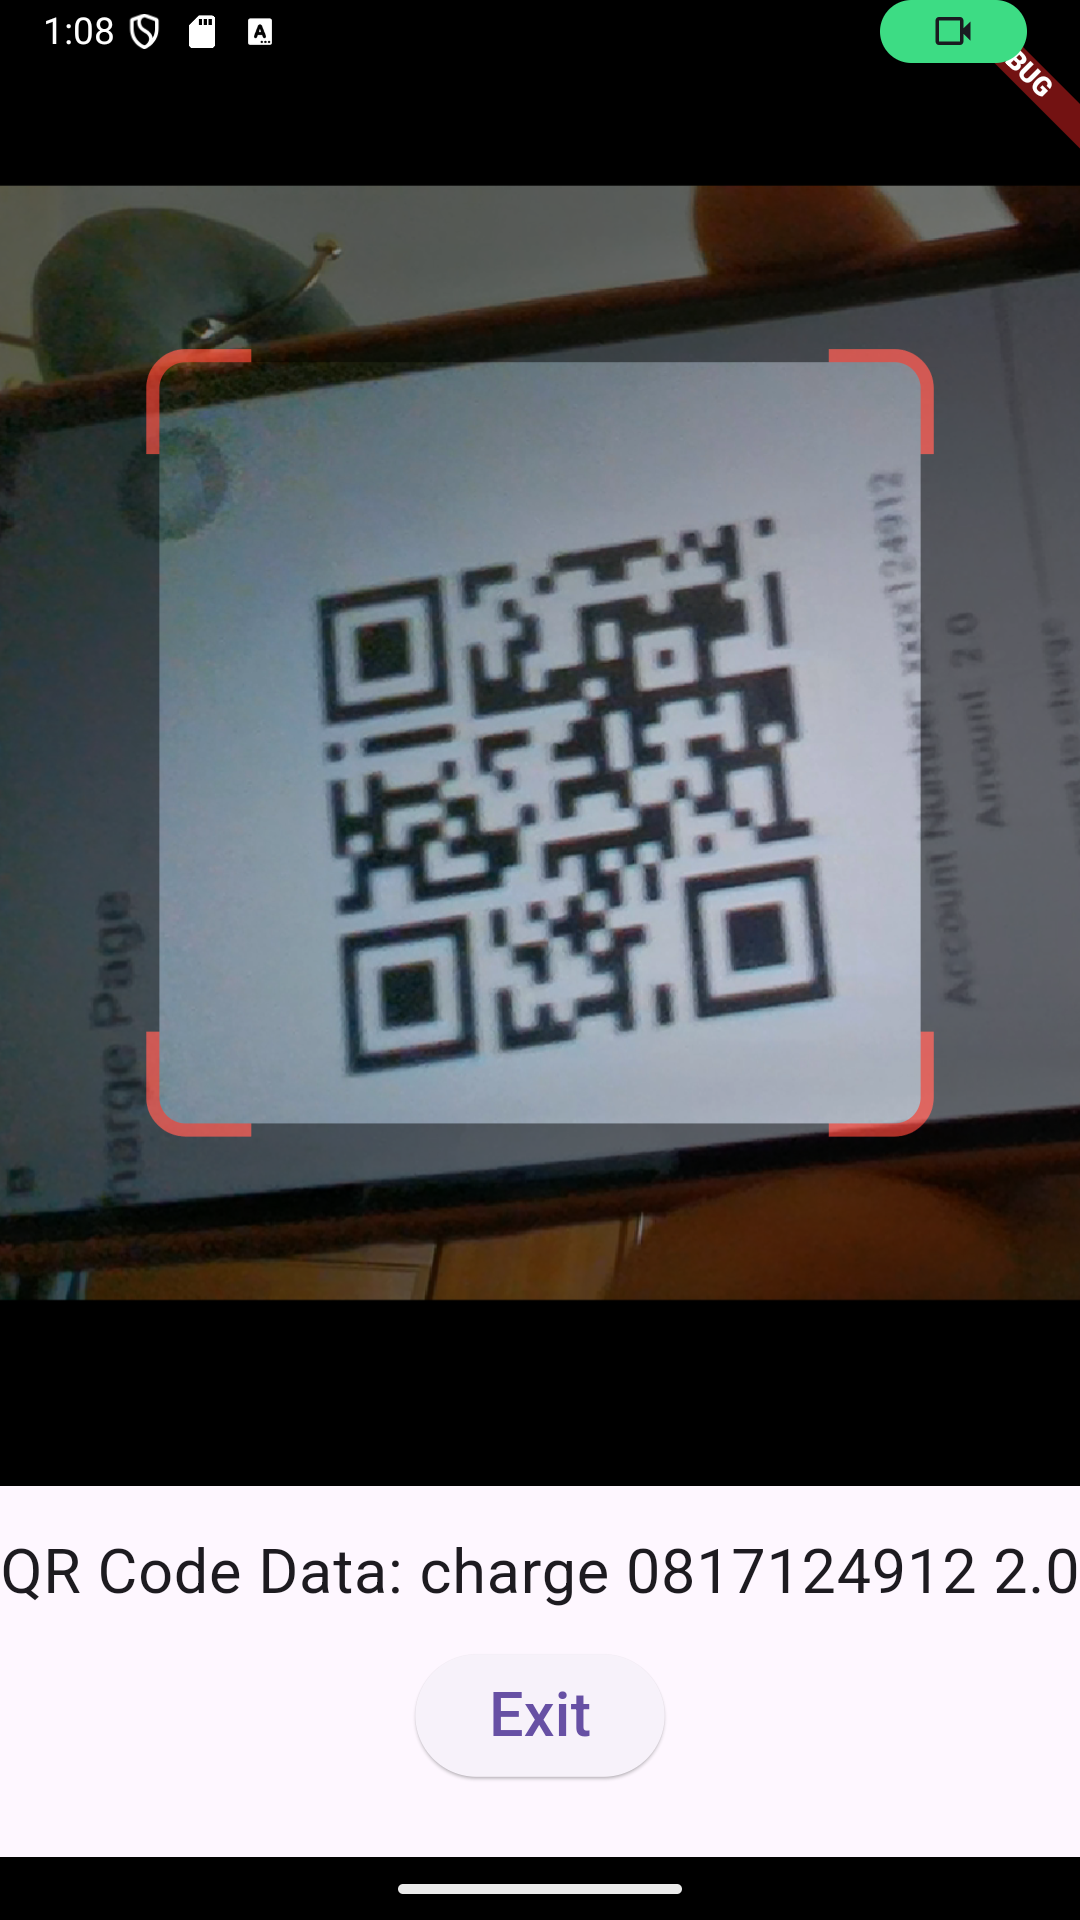
\includegraphics[width=\linewidth]{imatges/scanQR.png}
        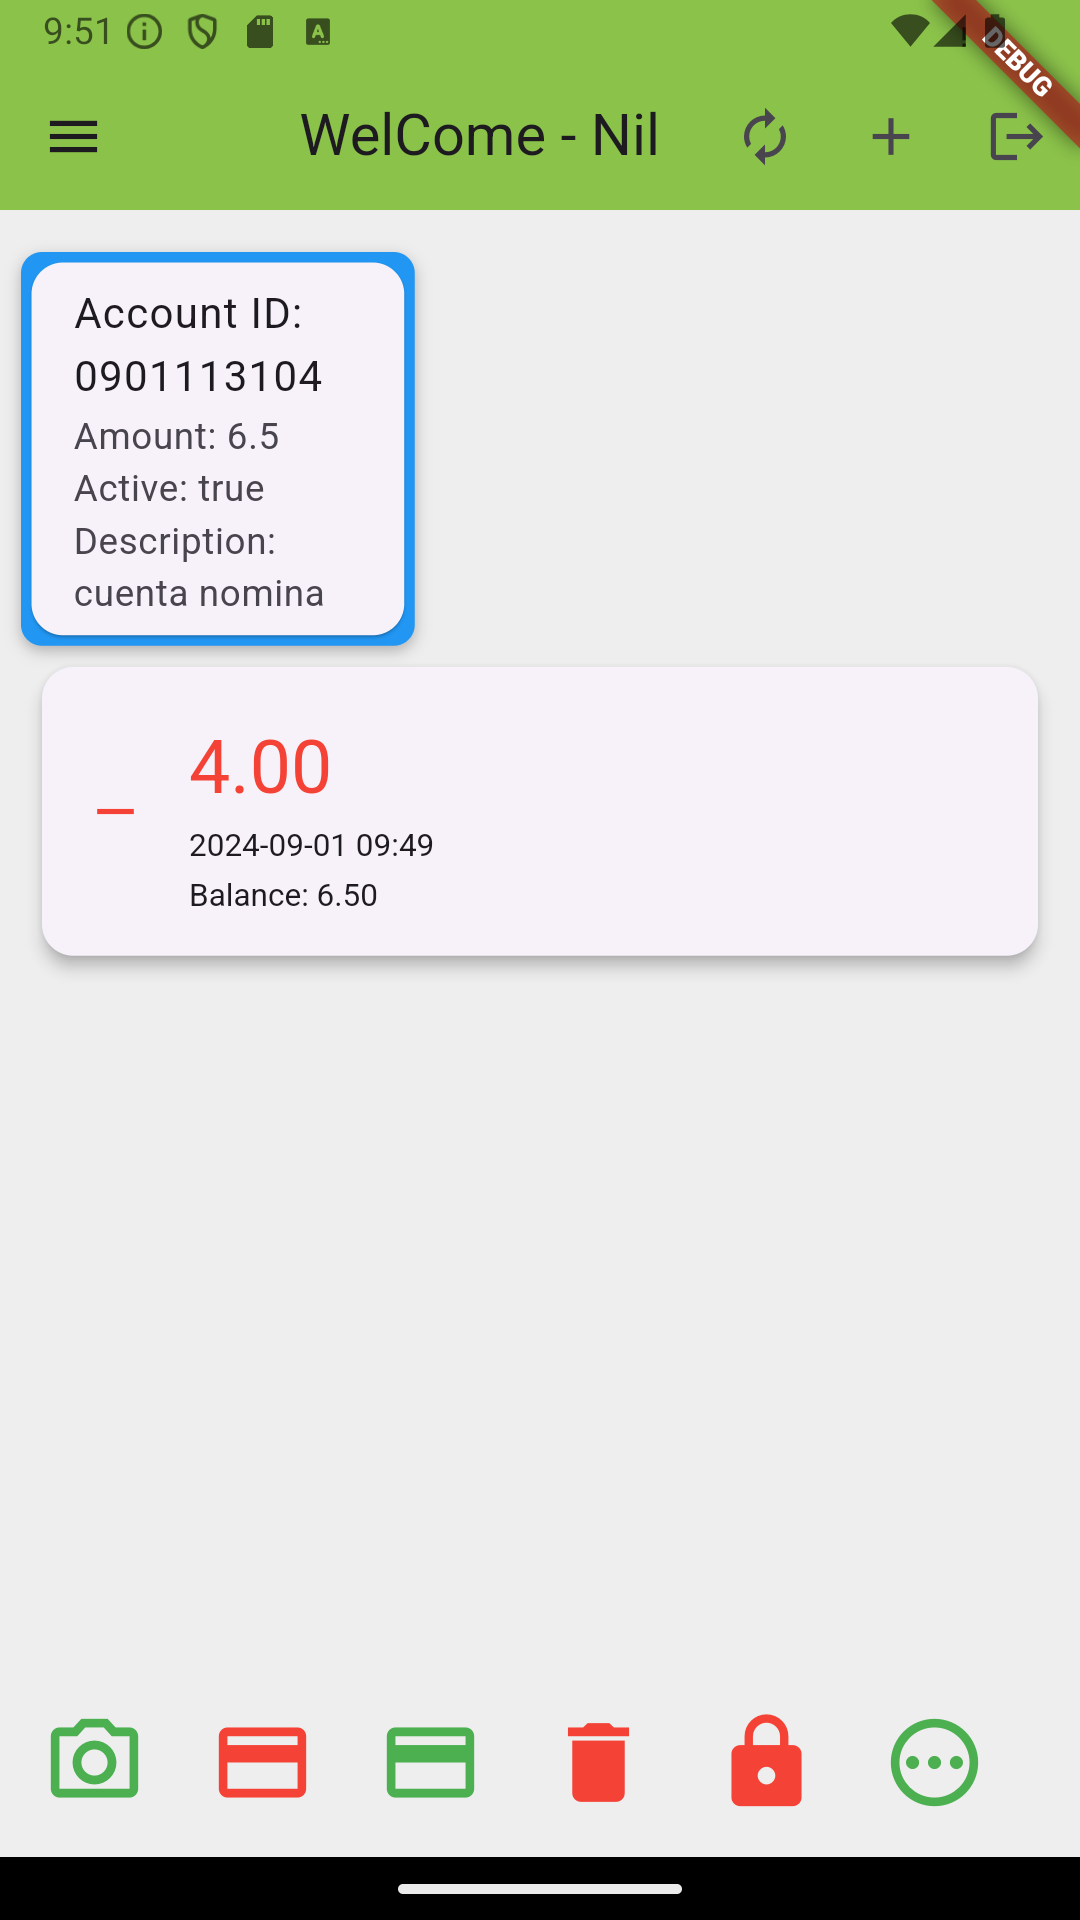
\includegraphics[width=\linewidth]{imatges/scanresult.png}
    \end{minipage}
    
    \caption{Escanejar codi QR}
    \label{fig:EscanejarCodiQR}
\end{figure}


\clearpage

\subsubsection{Pagina per generar codi QR de pagament}
\label{subsubsec:Pagina per generar codi QR de pagament}

Cal seleccionar un compte bancari per activar aquesta funció. En entrar a la pàgina, hi haurà dues opcions:

\begin{itemize} 
    \item Amb import introduït: el sistema fa una comprovació per assegurar-se que l'import és acceptable. 
    \item Sense import introduït: l'import serà introduït per la persona que escaneja, i després el sistema farà la comprovació. 
\end{itemize}

De totes maneres, el codi QR caducarà després d'un temps, només serà vàlid l'últim QR generat i només es podrà escanejar una sola vegada.

\begin{figure}[h]
    \centering
    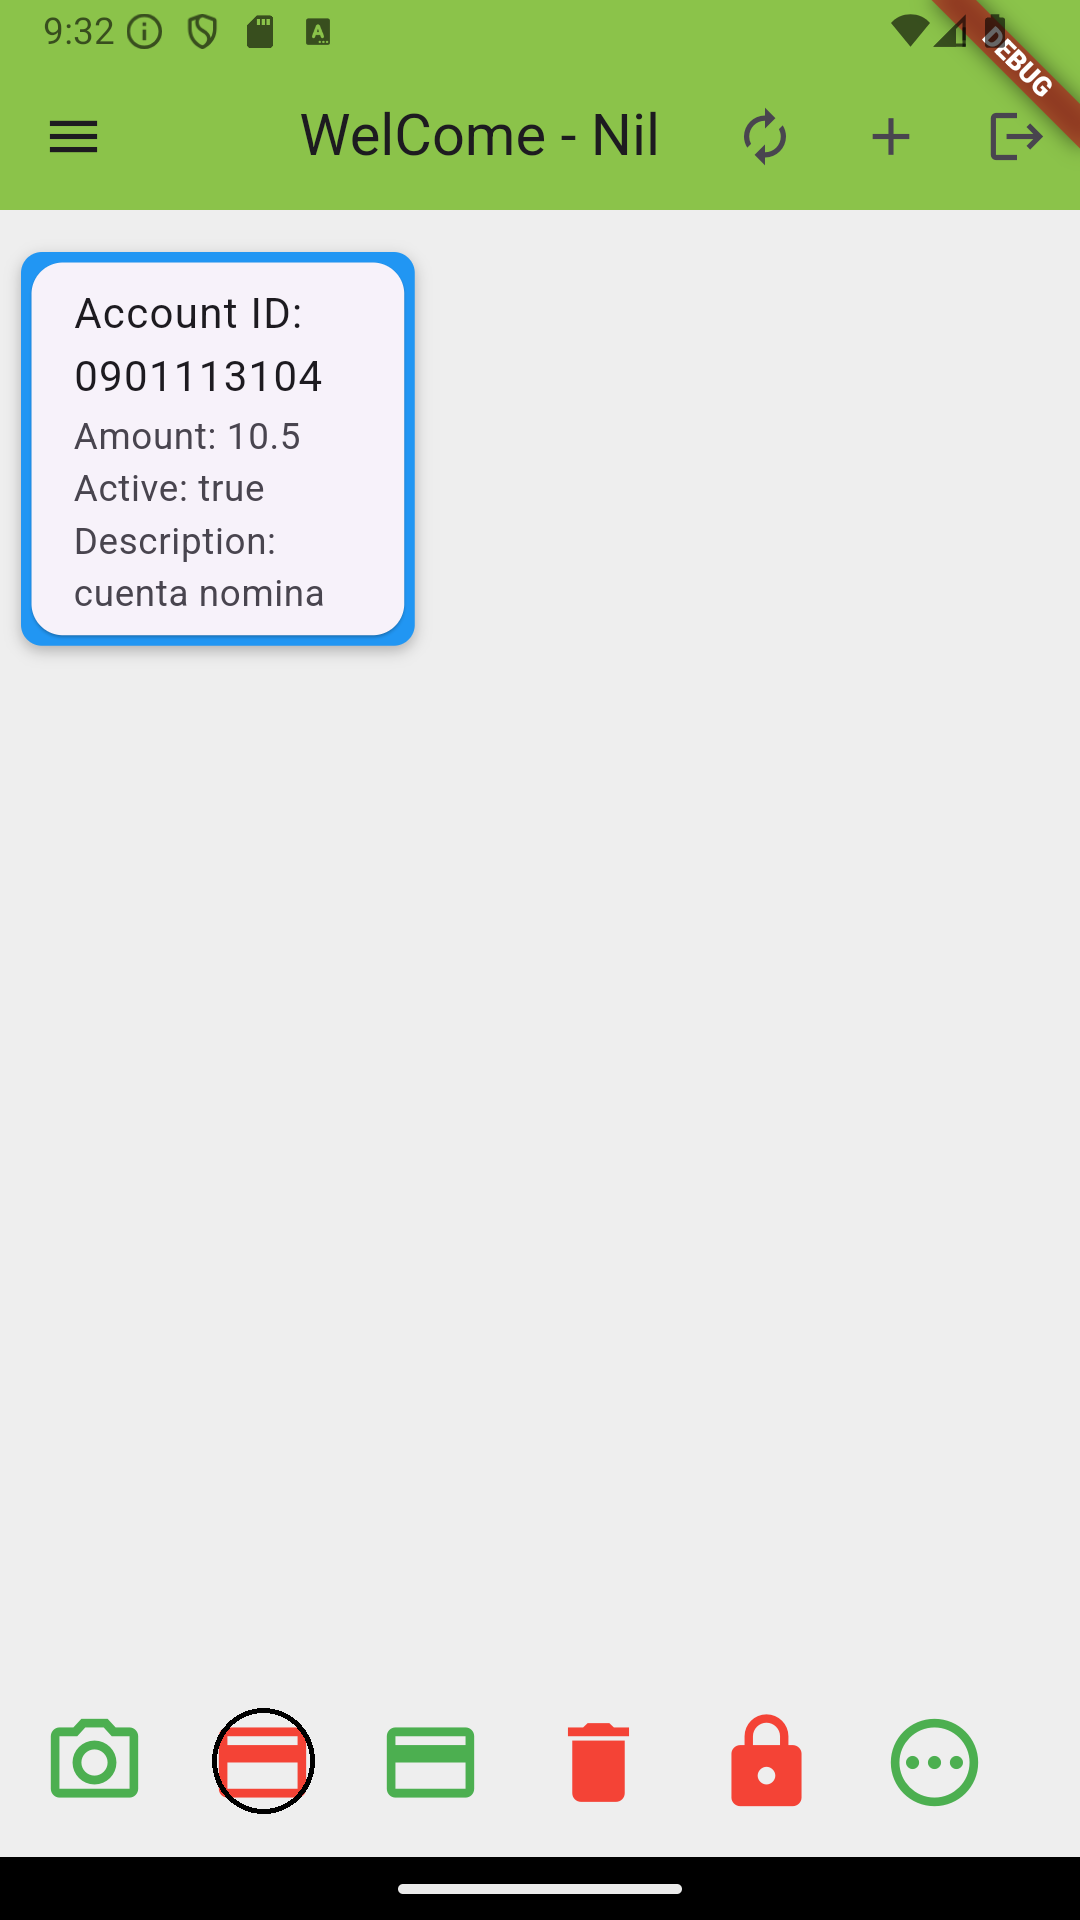
\includegraphics[width=0.32\textwidth]{imatges/mainpageAccount2.png}
    
\includegraphics[width=0.32\textwidth]{imatges/paymentPage.png}
    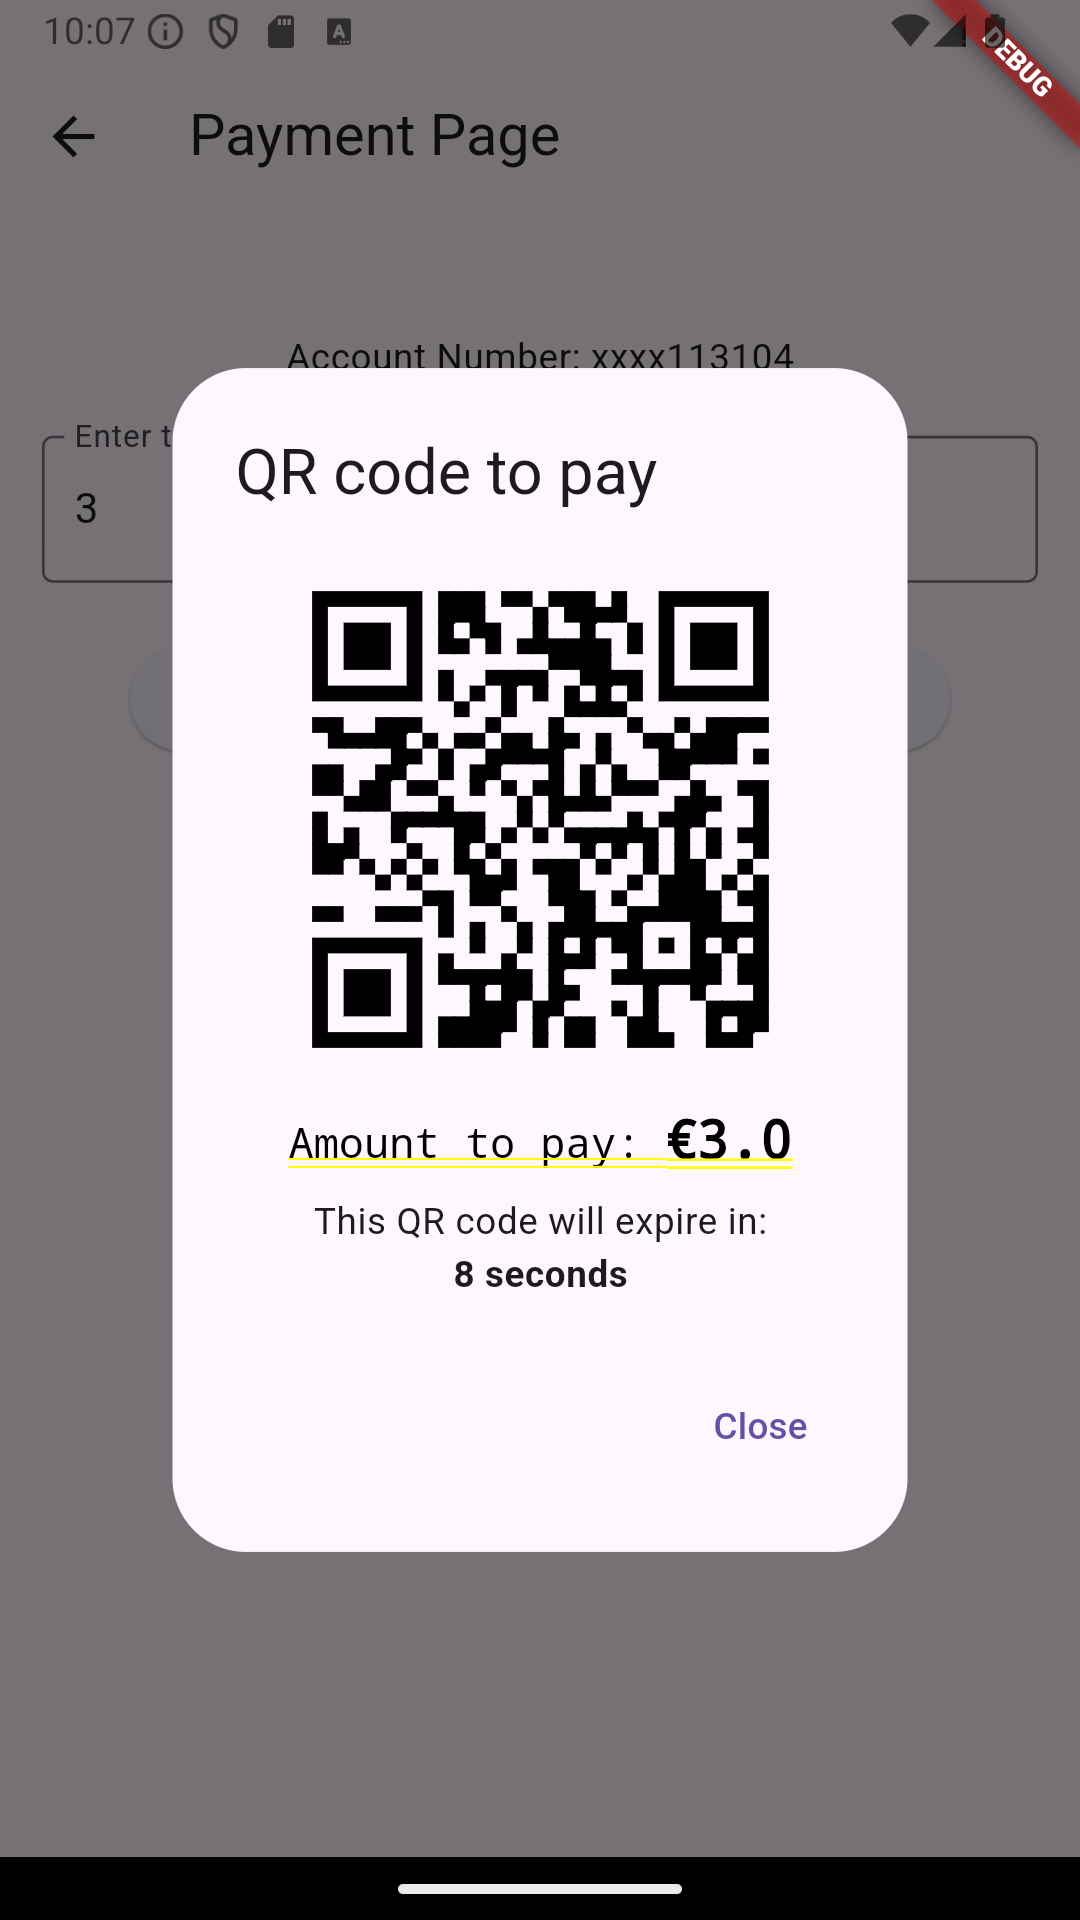
\includegraphics[width=0.32\textwidth]{imatges/paymentPageWithValue.png}
    \caption{Generar un codi QR de pagament.}
    \label{fig: Generar codi QR de pagament}
\end{figure}

\clearpage

\subsubsection{Generar codi QR de cobrament}
\label{subsubsec:Generar codi QR de cobrament}

És molt similar a la funcionalitat de "Generar un codi QR de pagament". Per defecte, en entrar a la pàgina, ja es mostra el codi QR de cobrament sense un import definit.\\

La diferència és que aquest codi QR de cobrament no caduca mai i es pot fer servir tantes vegades com es vulgui.

\begin{figure}[h]
    \centering
    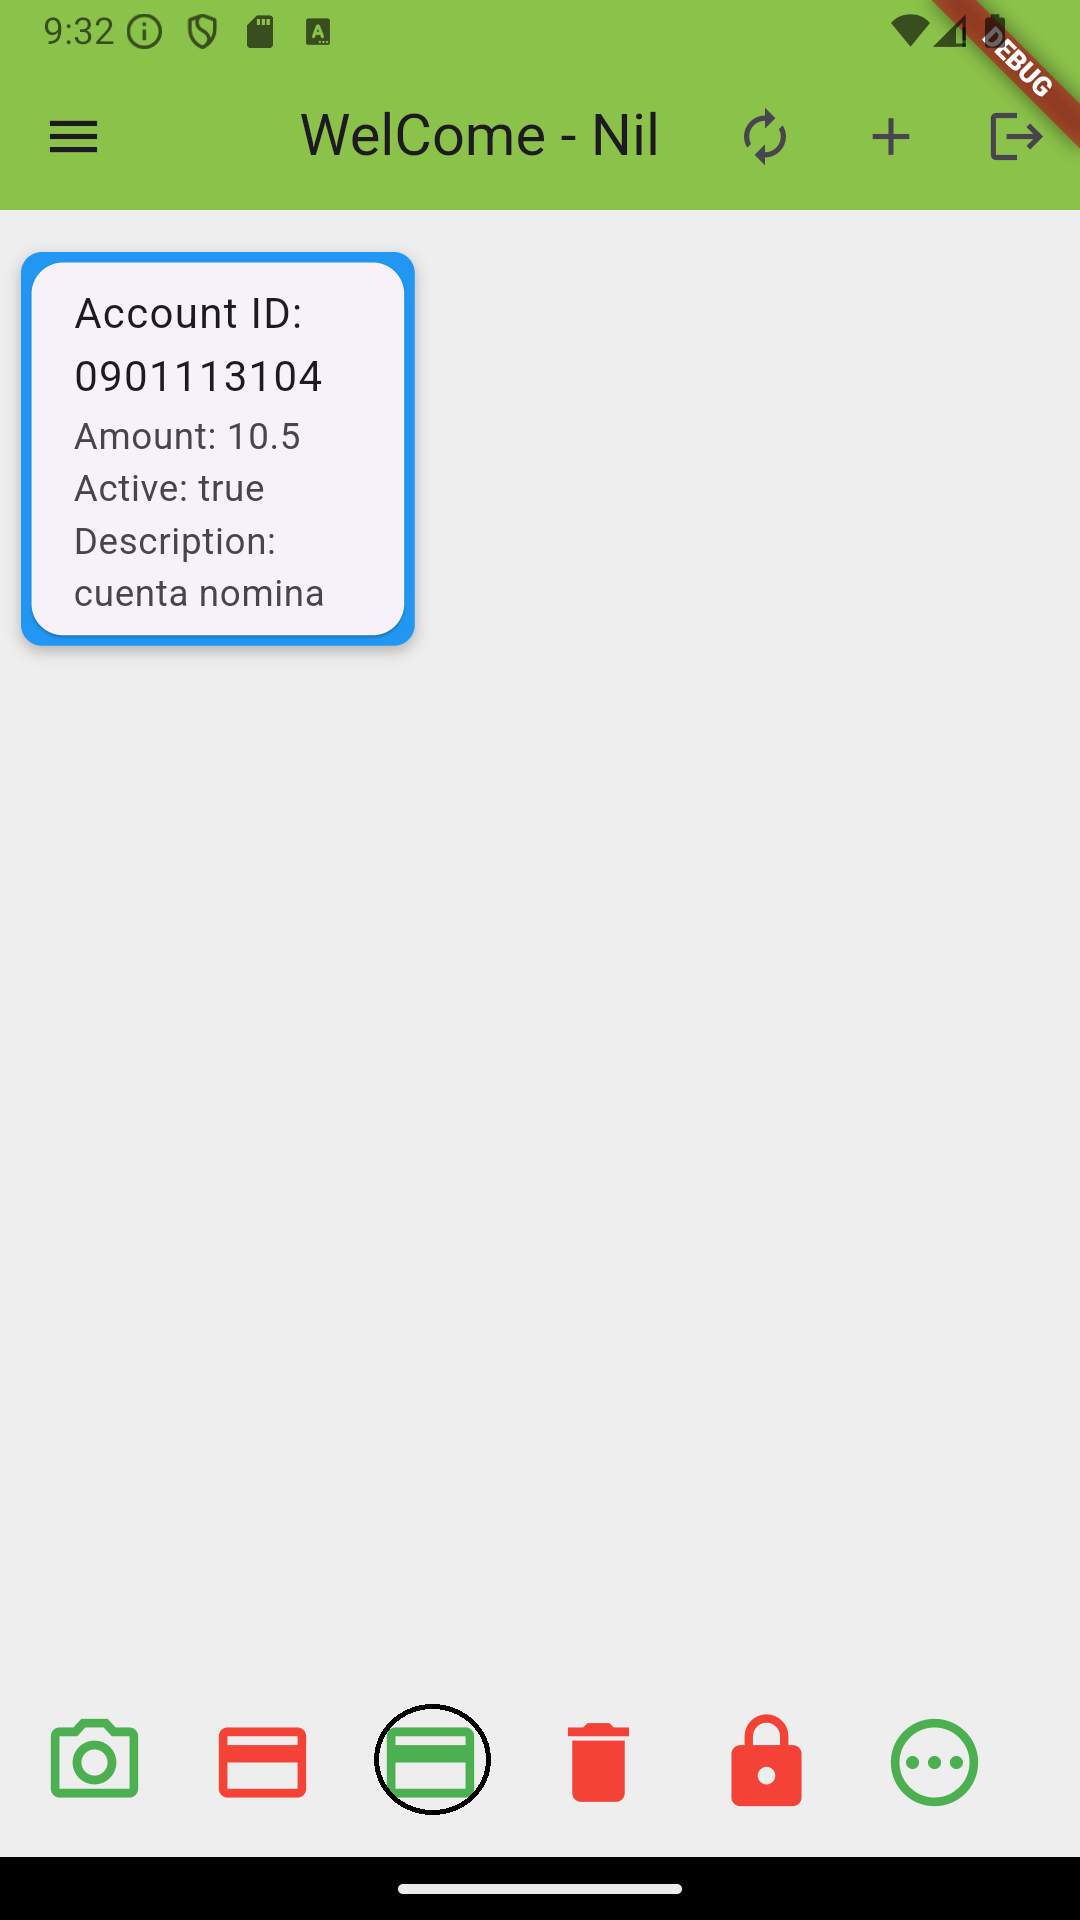
\includegraphics[width=0.32\textwidth]{imatges/mainpageAccount3.png}
    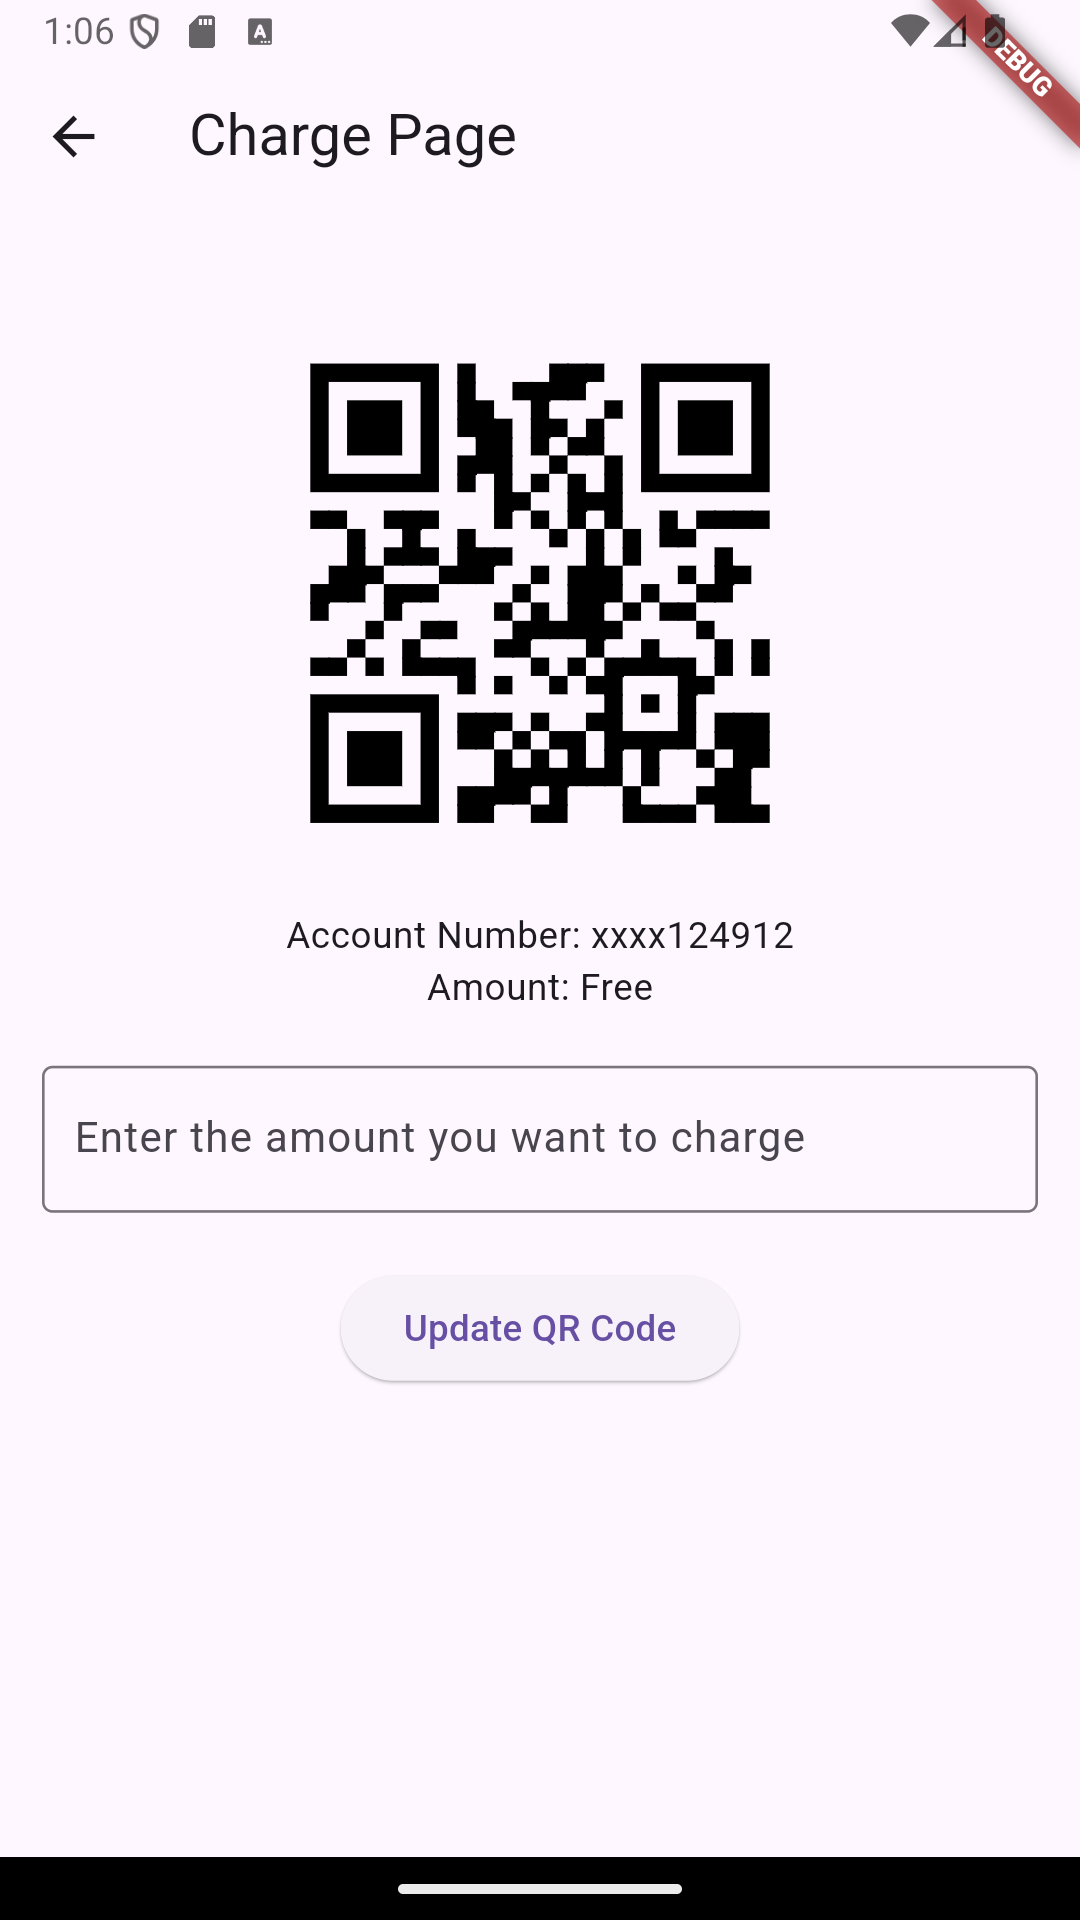
\includegraphics[width=0.32\textwidth]{imatges/chargePage.png}
    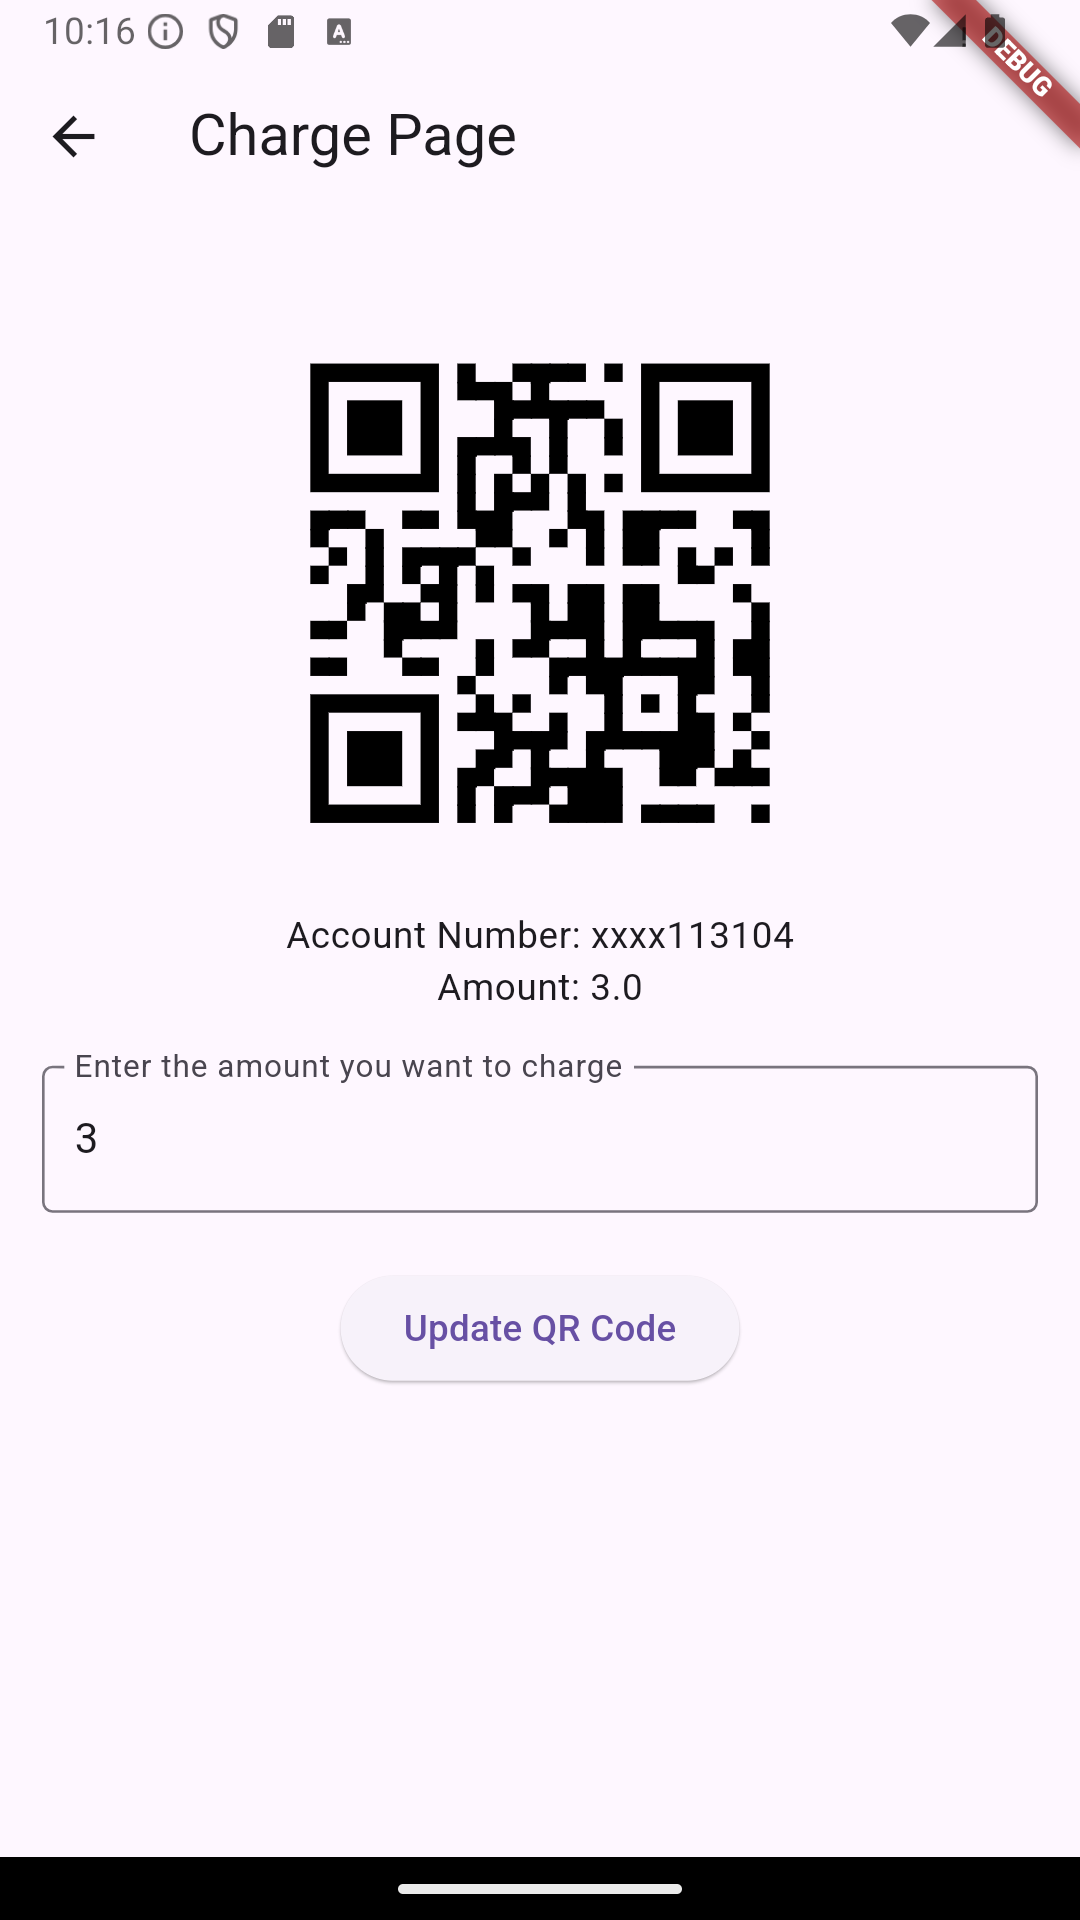
\includegraphics[width=0.32\textwidth]{imatges/chargePageWithValue.png}
    \caption{Pàgina per generar un codi QR de cobrament.}
    \label{fig: Pàgina per generar codi QR de cobrament}
\end{figure}

\clearpage

\subsubsection{Eliminar un compte bancari}
\label{subsubsec:Eliminar un compte bancari}

Per eliminar un compte bancari, cal que el saldo sigui 0. Si no és així, caldrà fer una transferència per deixar-lo a zero. Per facilitar-ho, l'app ofereix l'opció de fer transferències entre comptes bancaris del mateix client.

\begin{figure}[h]
    \centering
    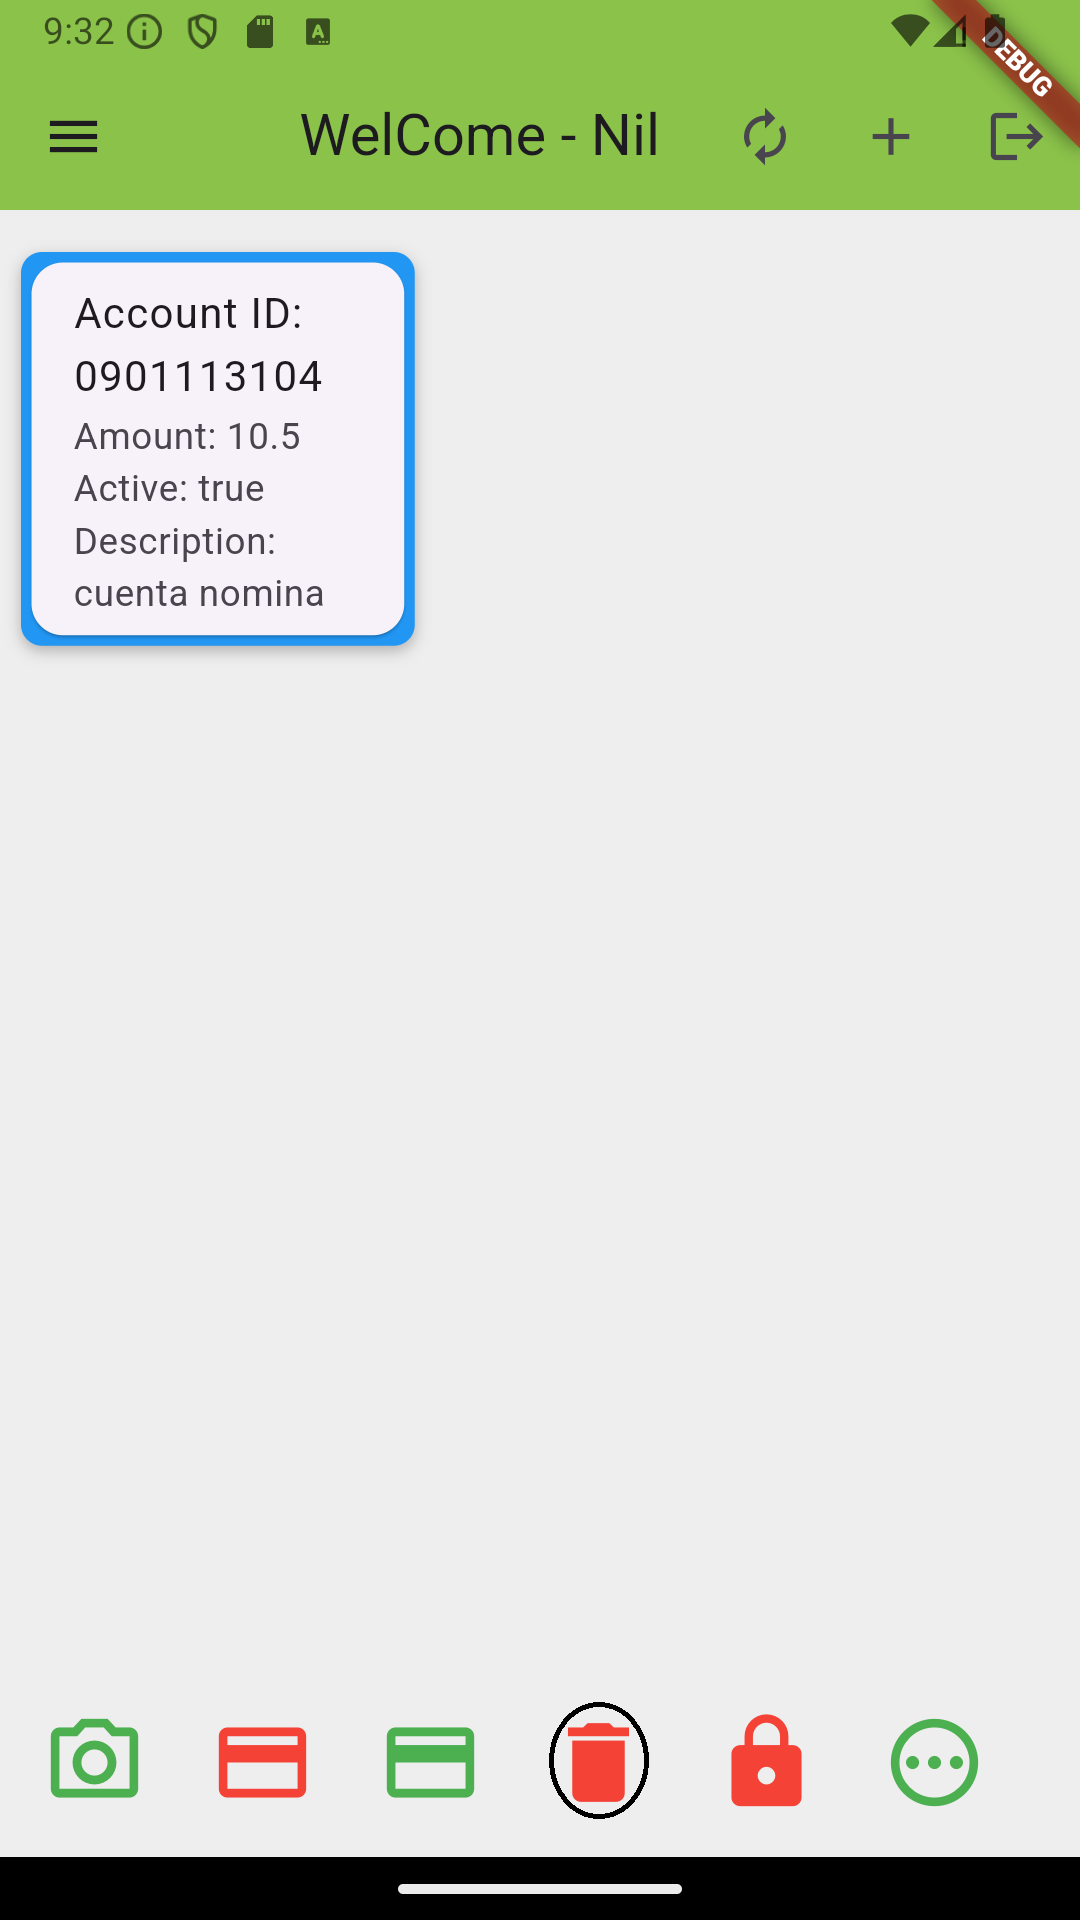
\includegraphics[width=0.32\textwidth]{imatges/mainpageAccount4.png}
    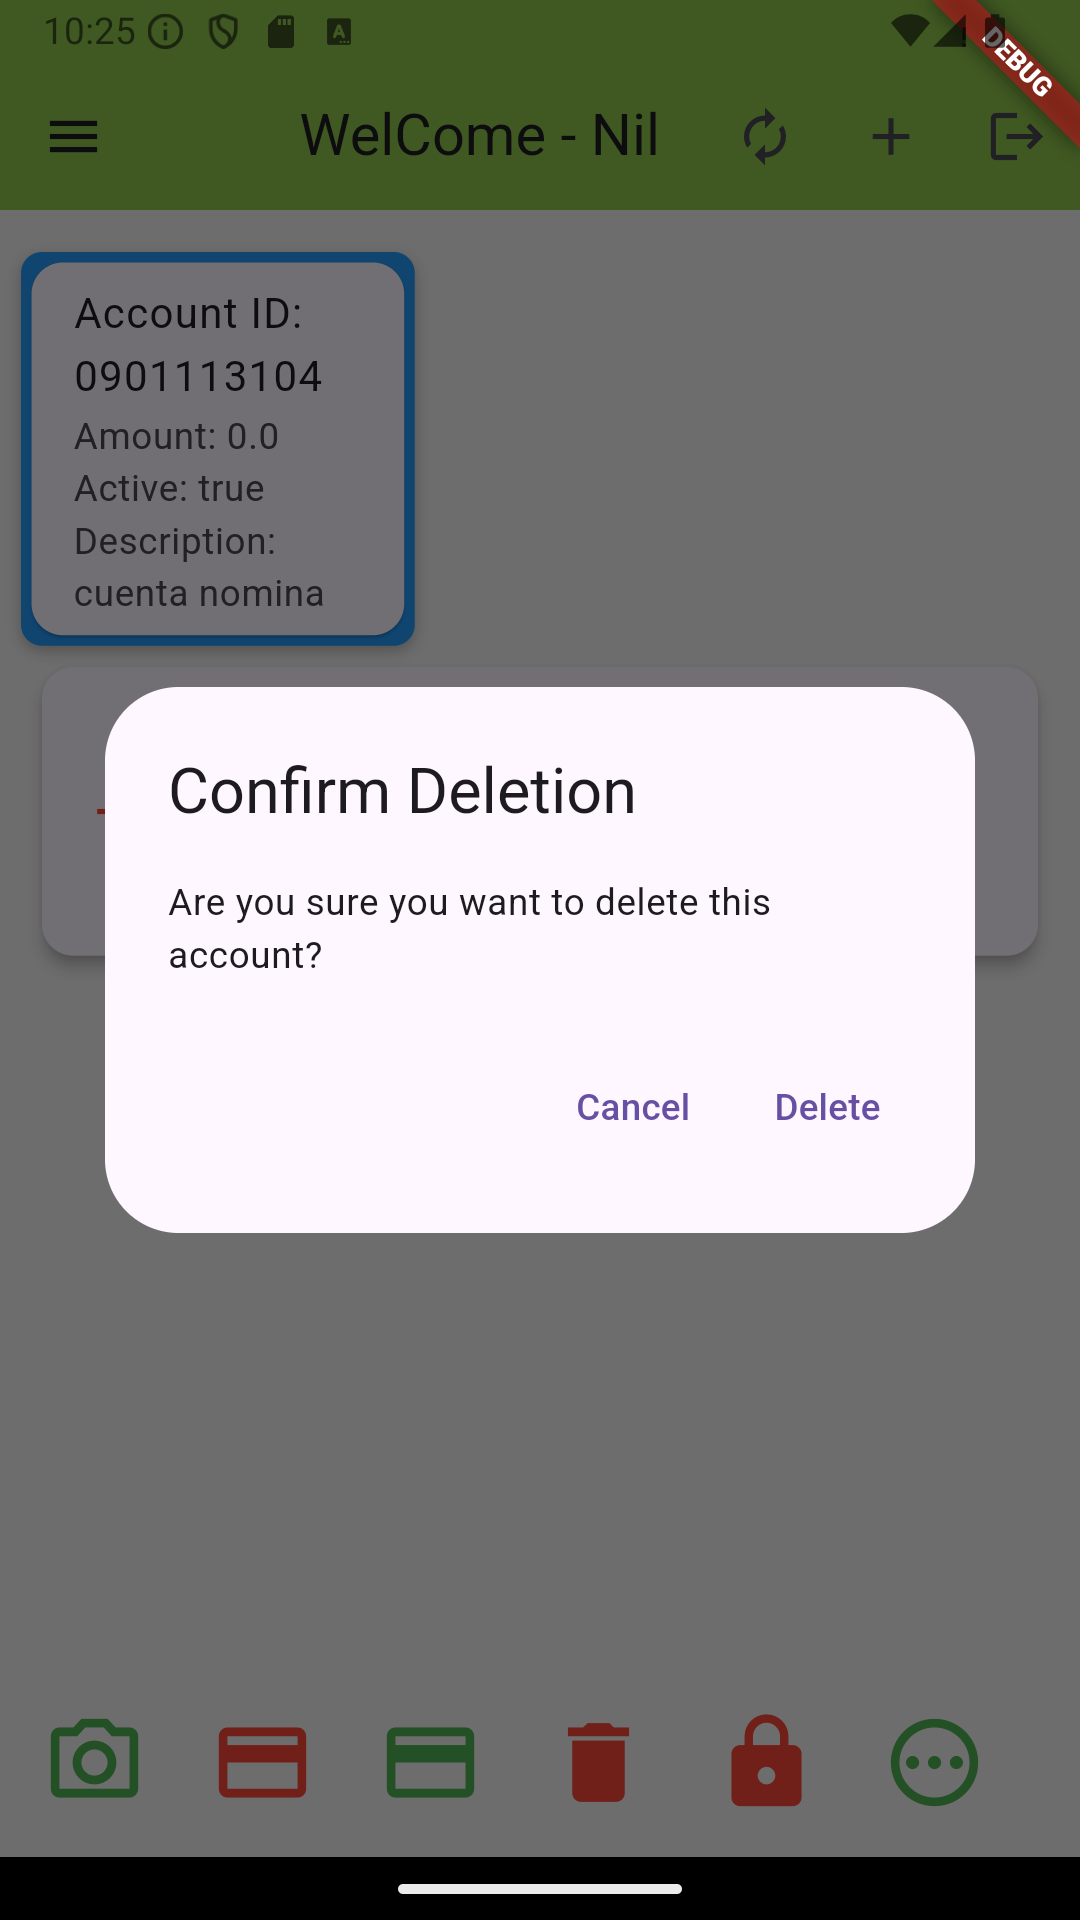
\includegraphics[width=0.32\textwidth]{imatges/deleteAccount.png}
    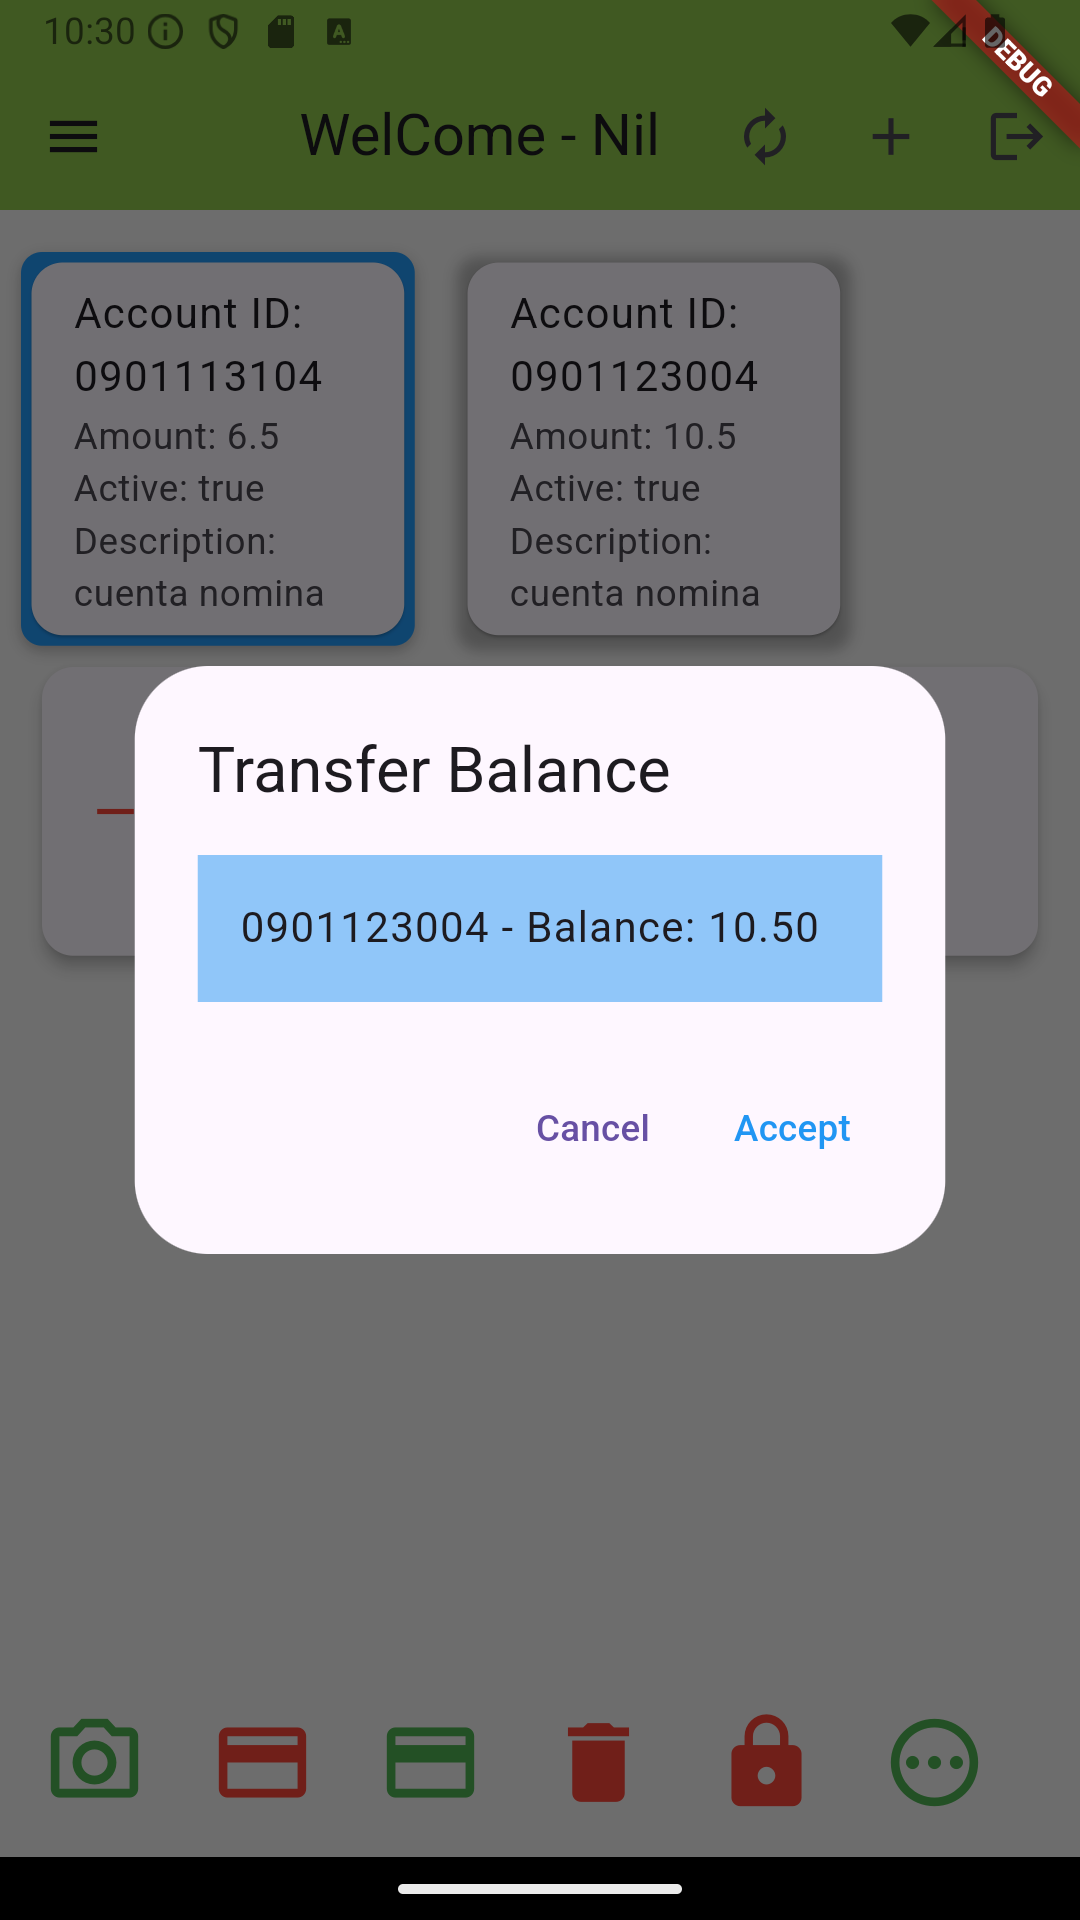
\includegraphics[width=0.32\textwidth]{imatges/transferBalance.png}
    \caption{Pàgina per generar un codi QR de cobrament.}
    \label{fig: Pàgina per generar codi QR de cobrament}
\end{figure}




\clearpage

\subsubsection{Modificar l'estat del compte bancari}
\label{subsubsec:Modificar l'estat del compte bancari}

Cal que hi hagi un compte seleccionat. Simplement clicant en l'icona del cadenat, es canviarà l'estat del compte bancari. Si està en estat de desactivat, no es podrà generar un QR de pagament ni efectuar cap pagament.

El cadenat es tanca o obre segons l'estat.

\begin{figure}[h]
    \centering
    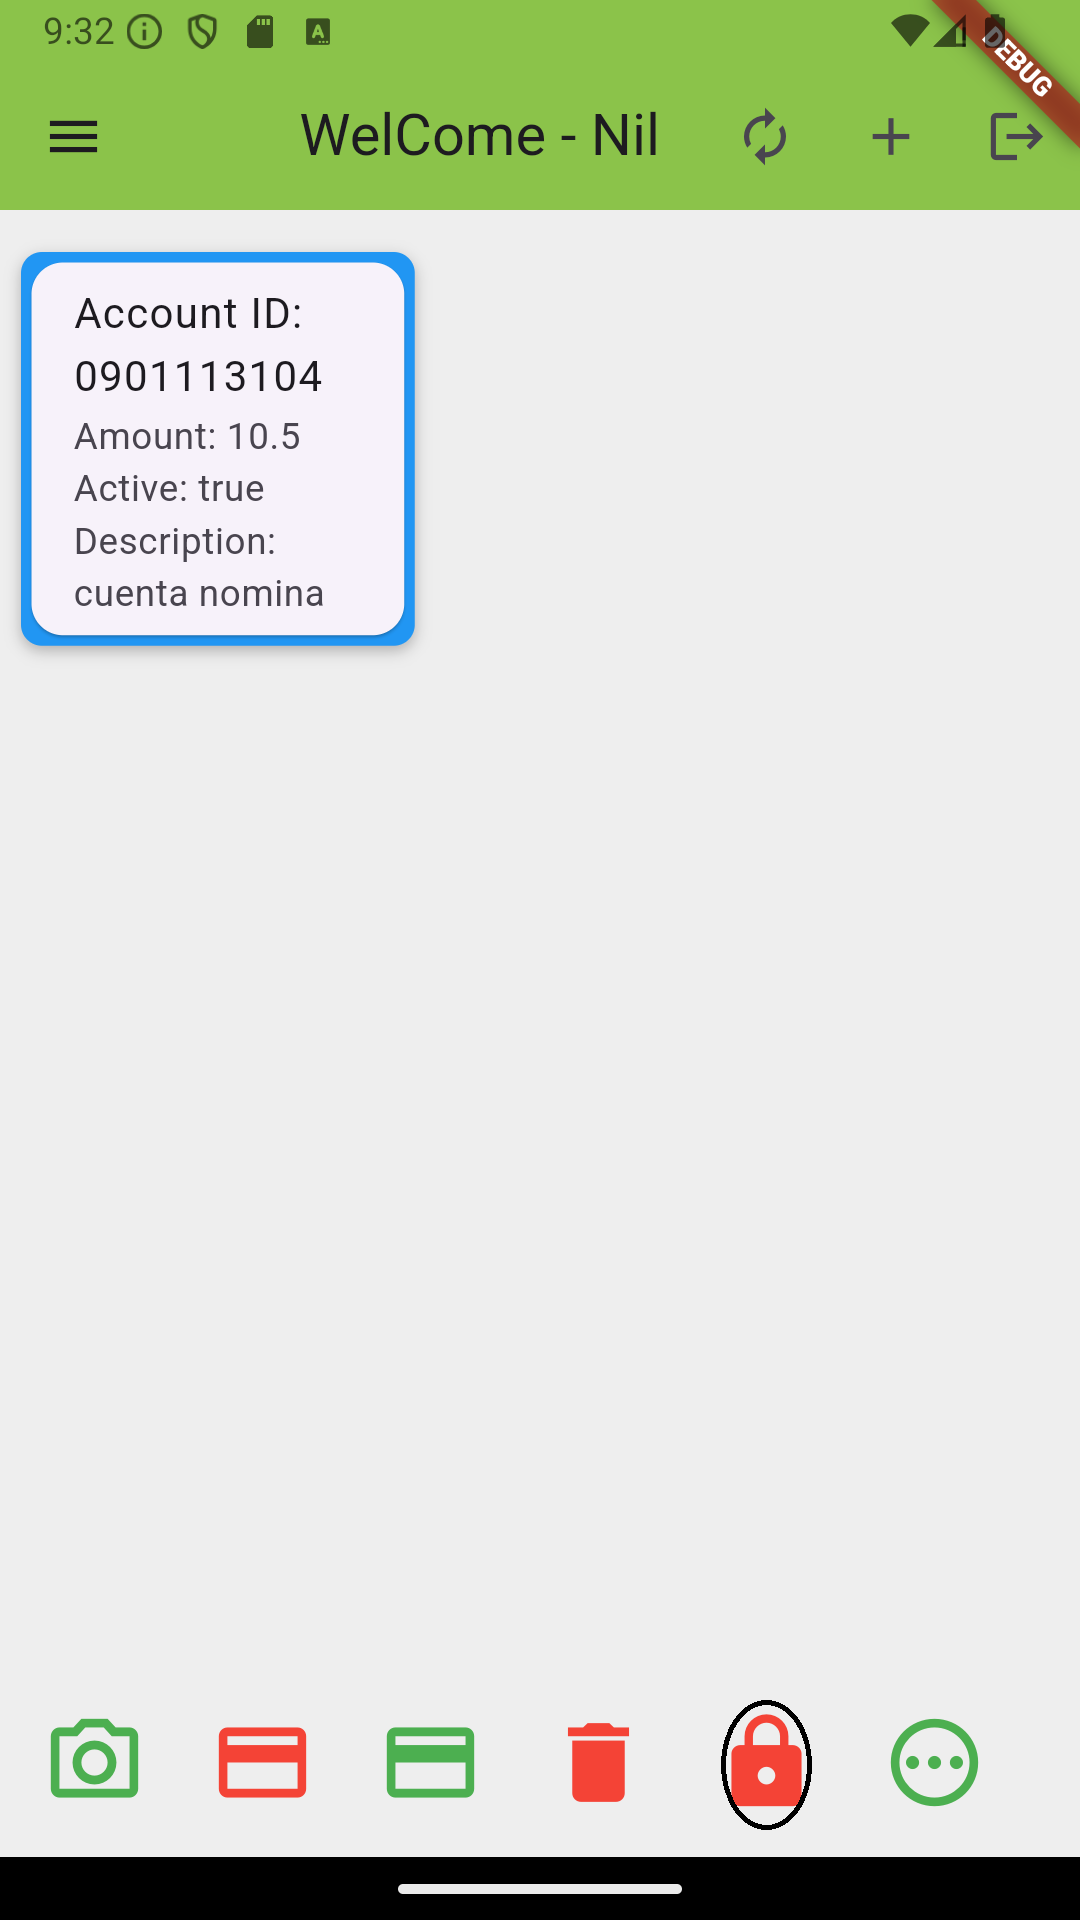
\includegraphics[width=0.32\textwidth]{imatges/mainpageAccount5.png}
    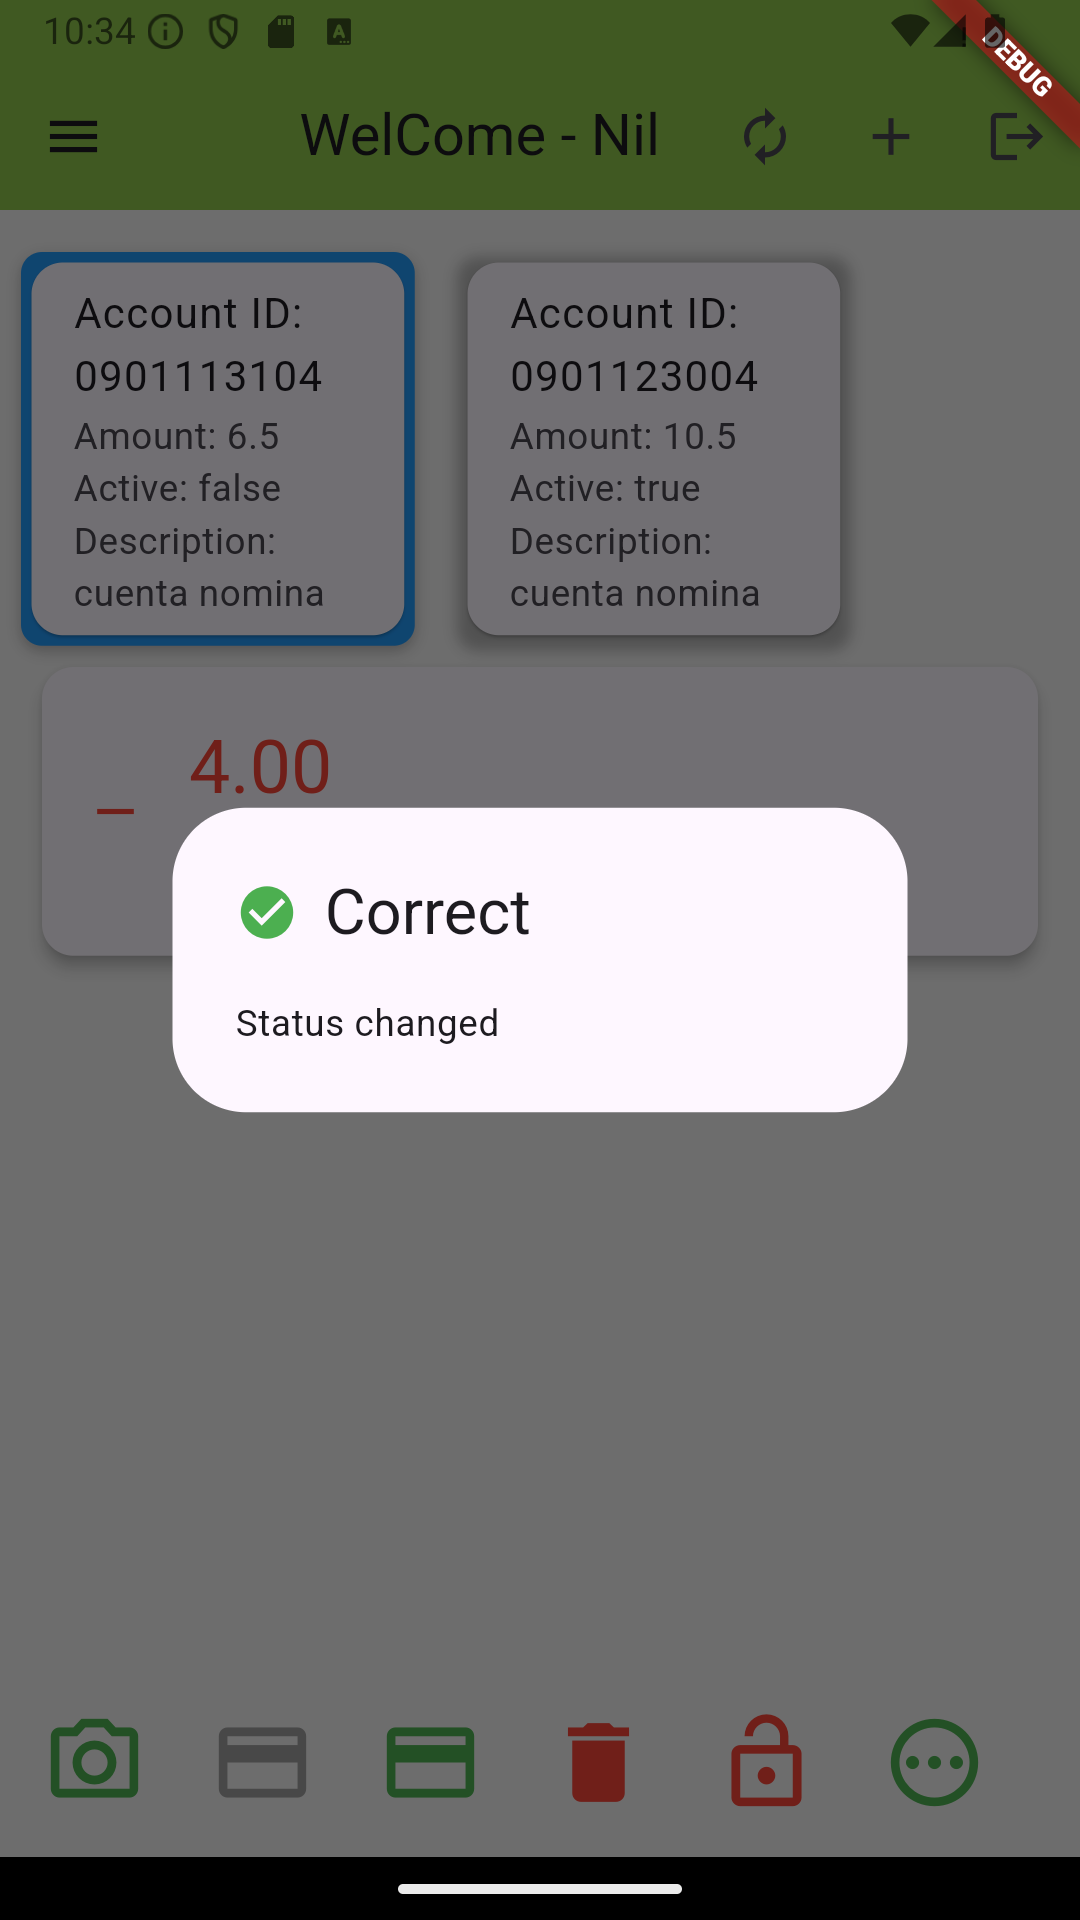
\includegraphics[width=0.32\textwidth]{imatges/changeStatus1.png}
    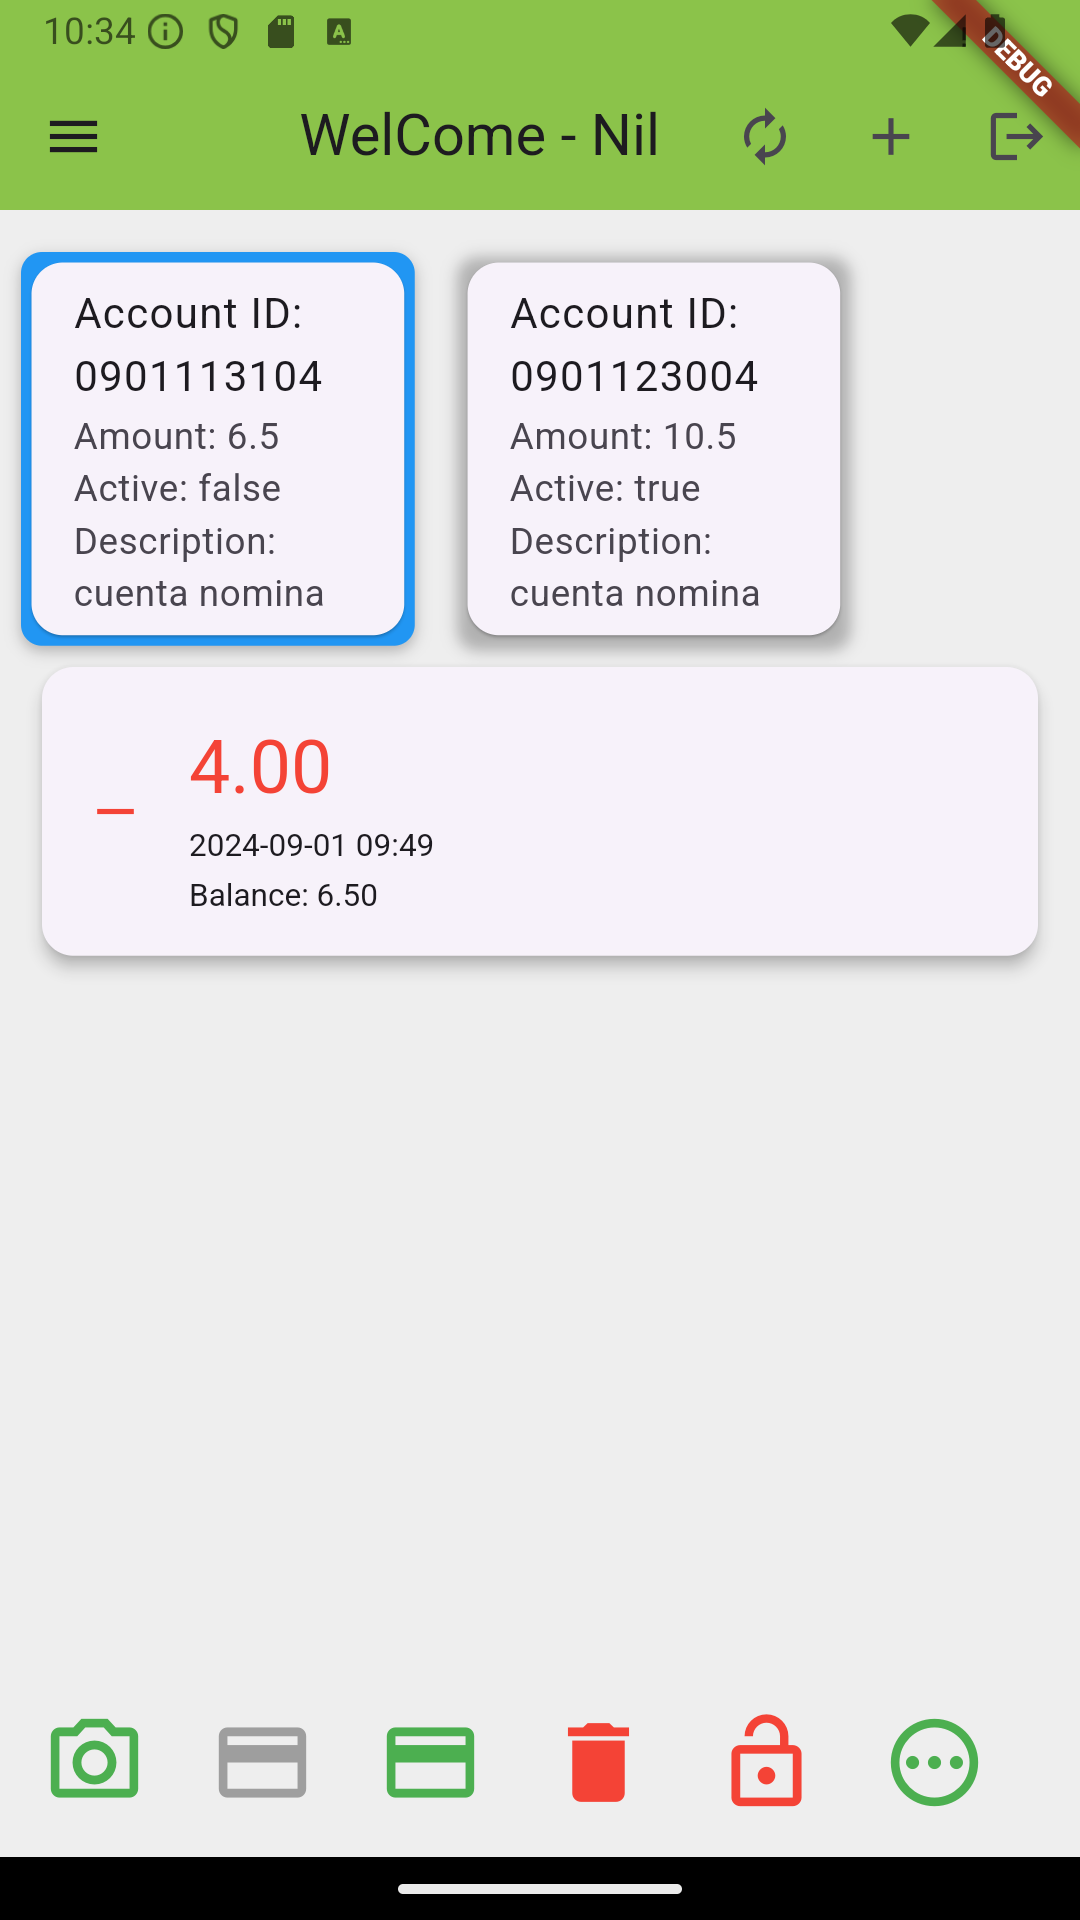
\includegraphics[width=0.32\textwidth]{imatges/changeStatus2.png}
    \caption{Modificar l'estat del compte bancari}
    \label{fig: Modificar l'estat del compte bancari}
\end{figure}


\clearpage

\subsubsection{Altres operacions sobre el compte bancari}
\label{subsubsec:Altres operacions sobre el compte bancari}


A més de les funcionalitats bàsiques, també es poden realitzar les següents operacions sobre el compte bancari:

\begin{itemize} 
    \item Fer transaccions manualment sense generar ni escanejar un codi QR. 
    \item Definir el nou límit de pagament per transacció. 
    \item Definir una nova descripció per al compte bancari.
\end{itemize}


\begin{figure}[h]
    \centering
    % Primera fila amb 2 imatges
    \begin{minipage}{0.30\textwidth}
        \centering
        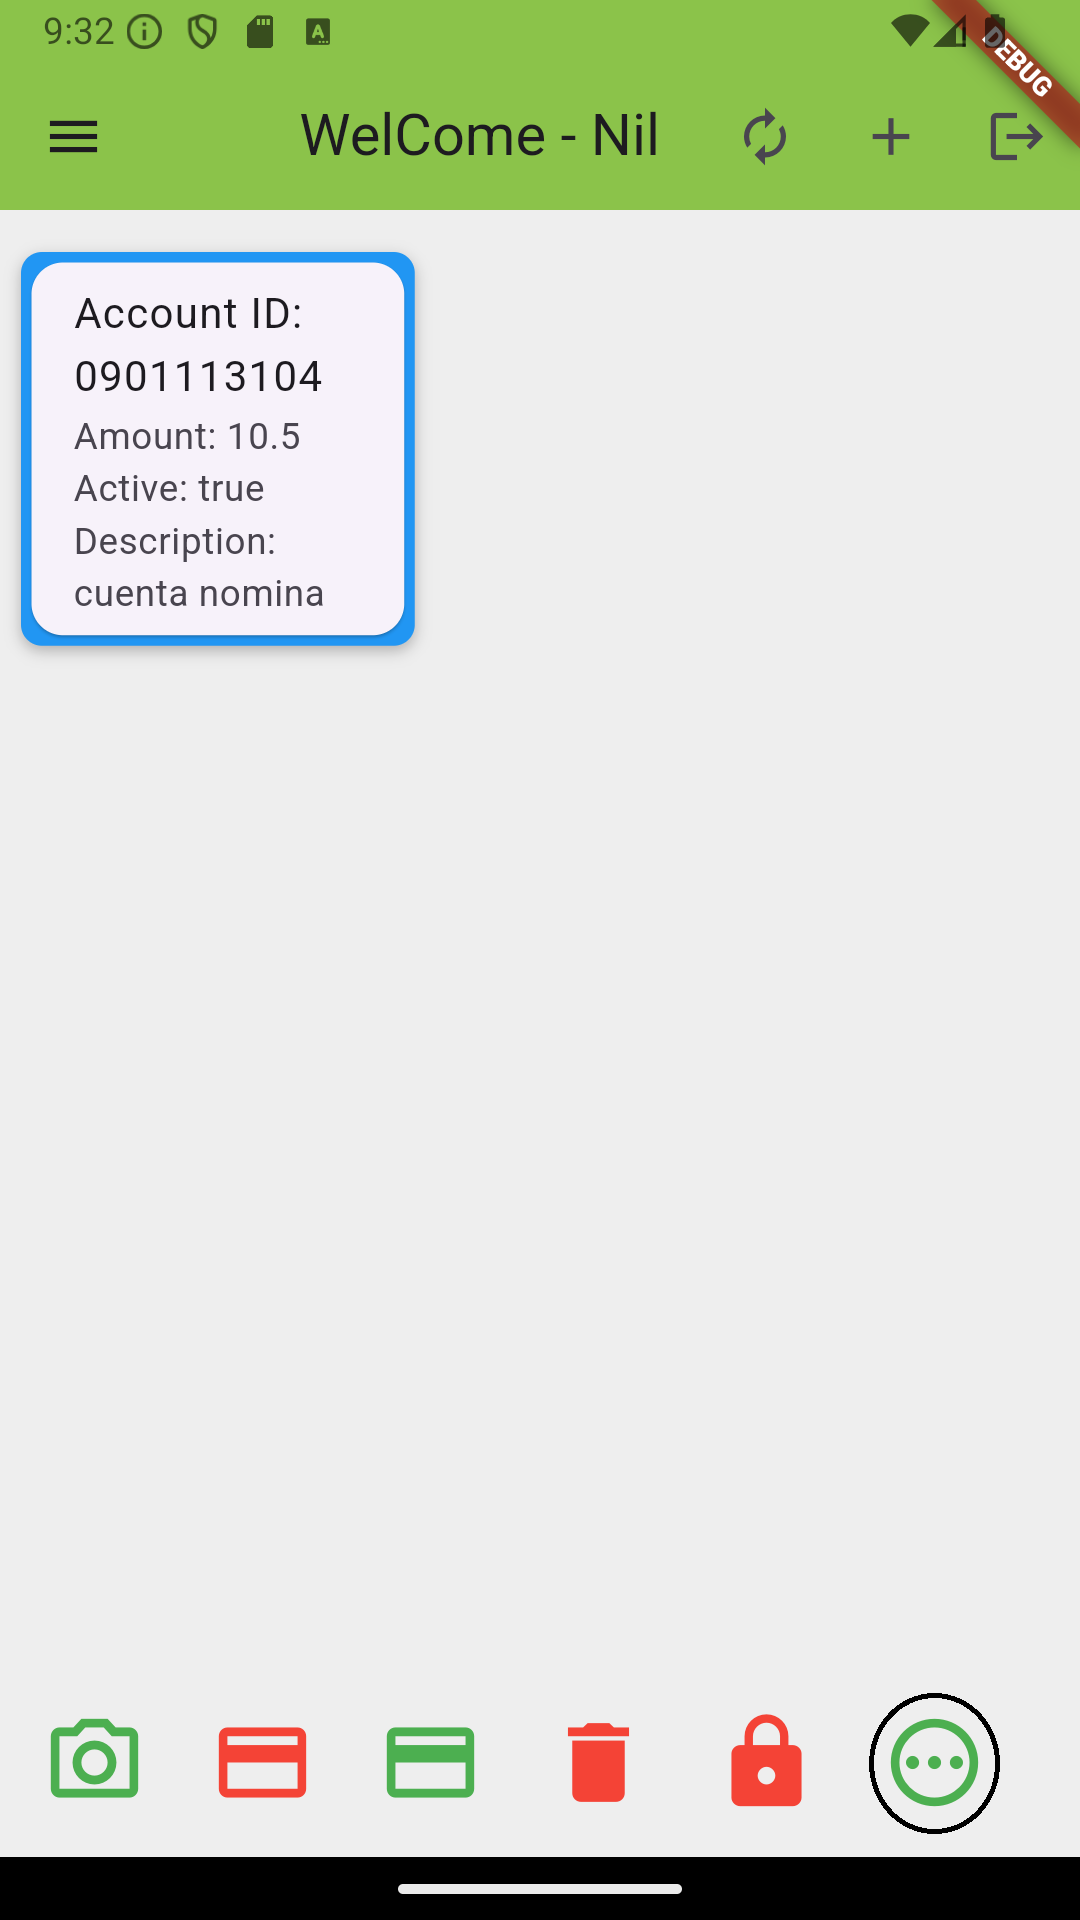
\includegraphics[width=\textwidth]{imatges/mainpageAccount6.png}
    \end{minipage}
    \begin{minipage}{0.30\textwidth}
        \centering
        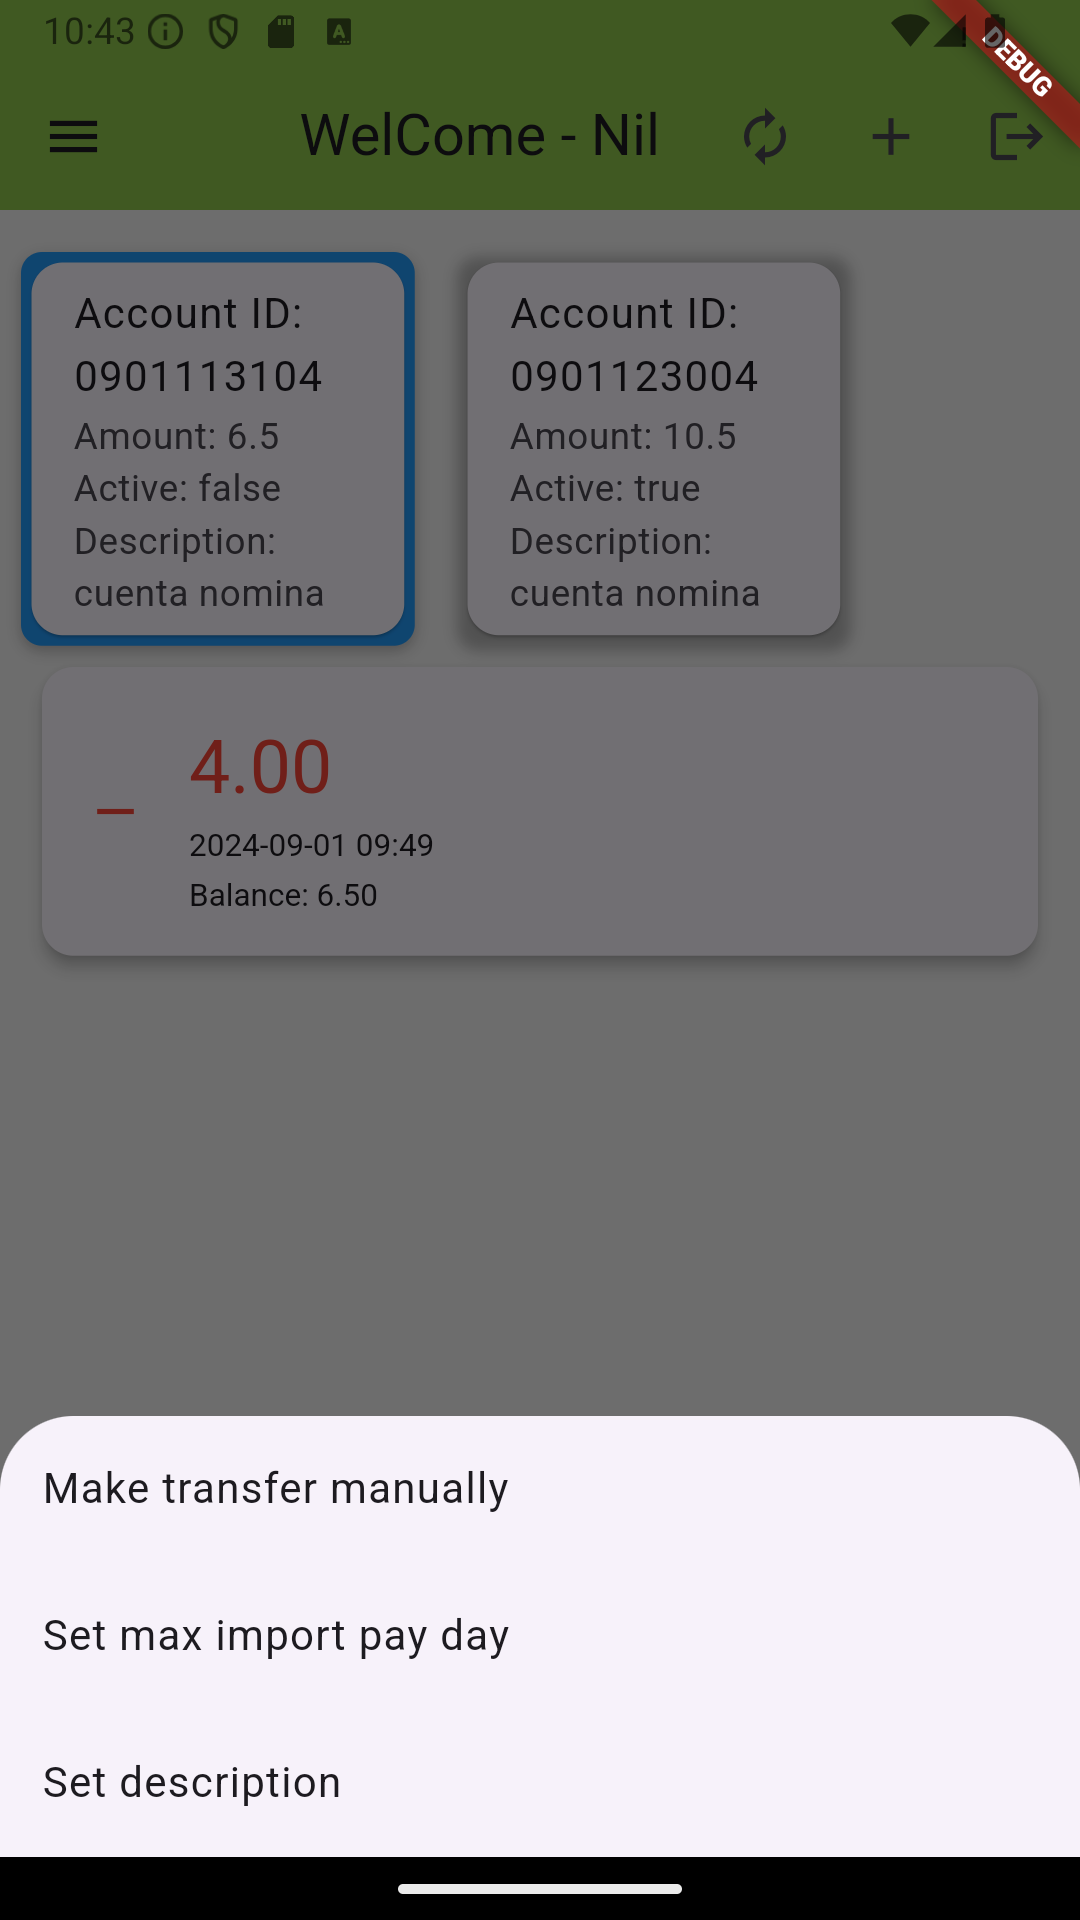
\includegraphics[width=\textwidth]{imatges/otherOperation.png}
    \end{minipage}

    % Espai entre files
    \vspace{1em}

    % Segona fila amb 3 imatges
    \begin{minipage}{0.30\textwidth}
        \centering
        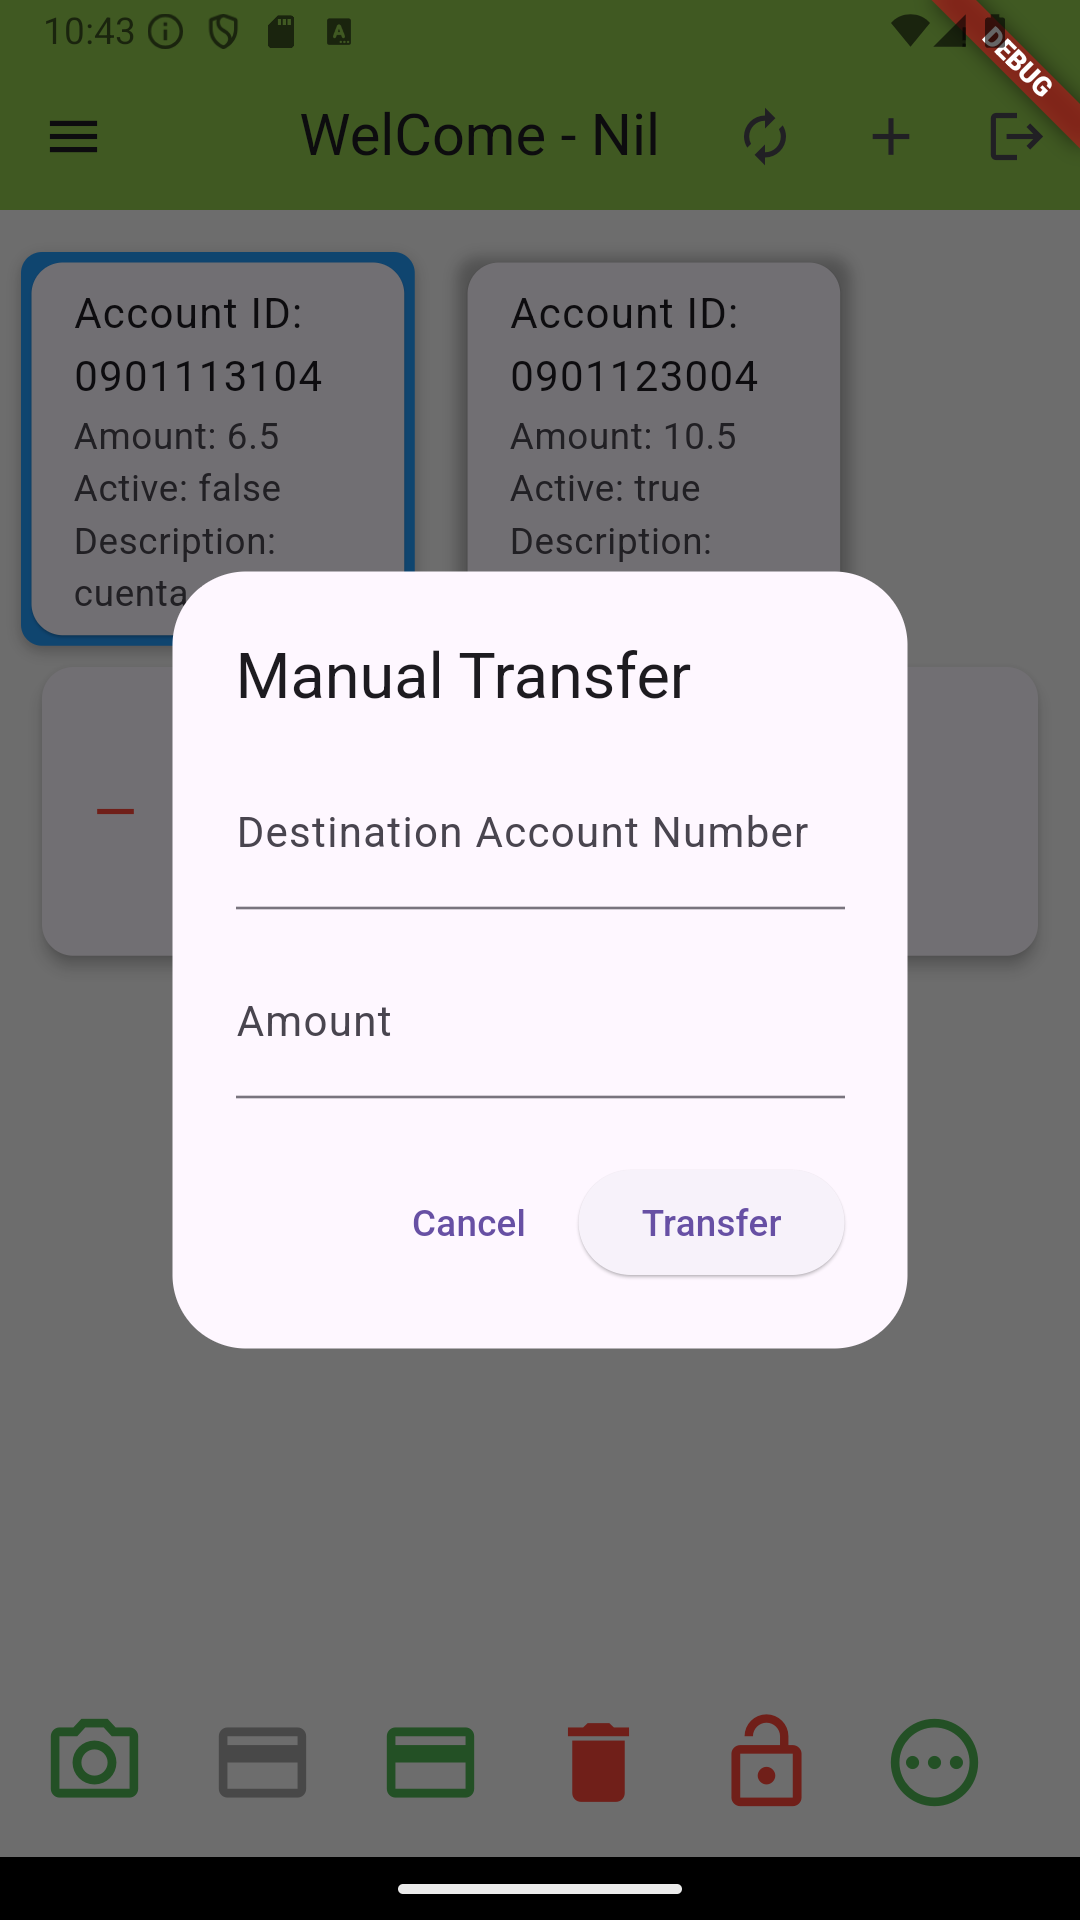
\includegraphics[width=\textwidth]{imatges/otherOperation1.png}
    \end{minipage}
    \begin{minipage}{0.30\textwidth}
        \centering
        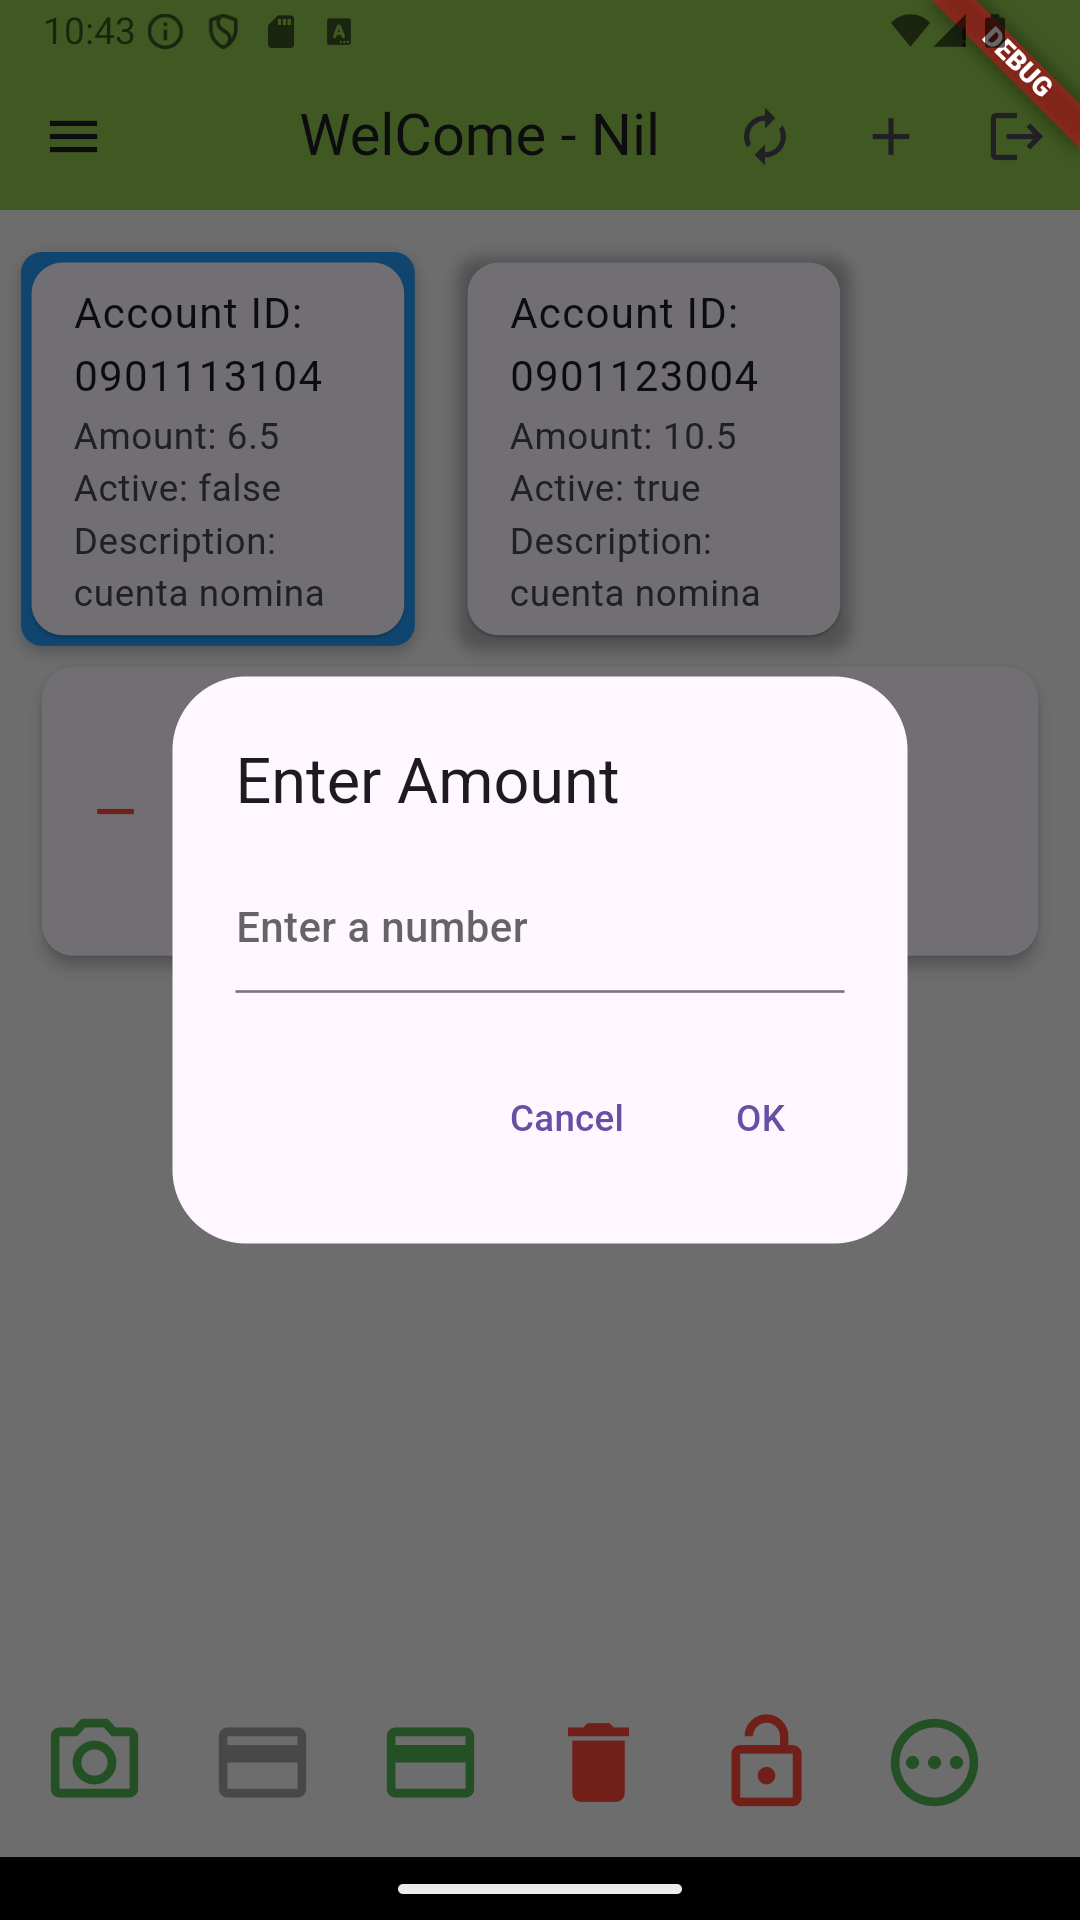
\includegraphics[width=\textwidth]{imatges/otherOperation2.png}
    \end{minipage}
    \begin{minipage}{0.30\textwidth}
        \centering
        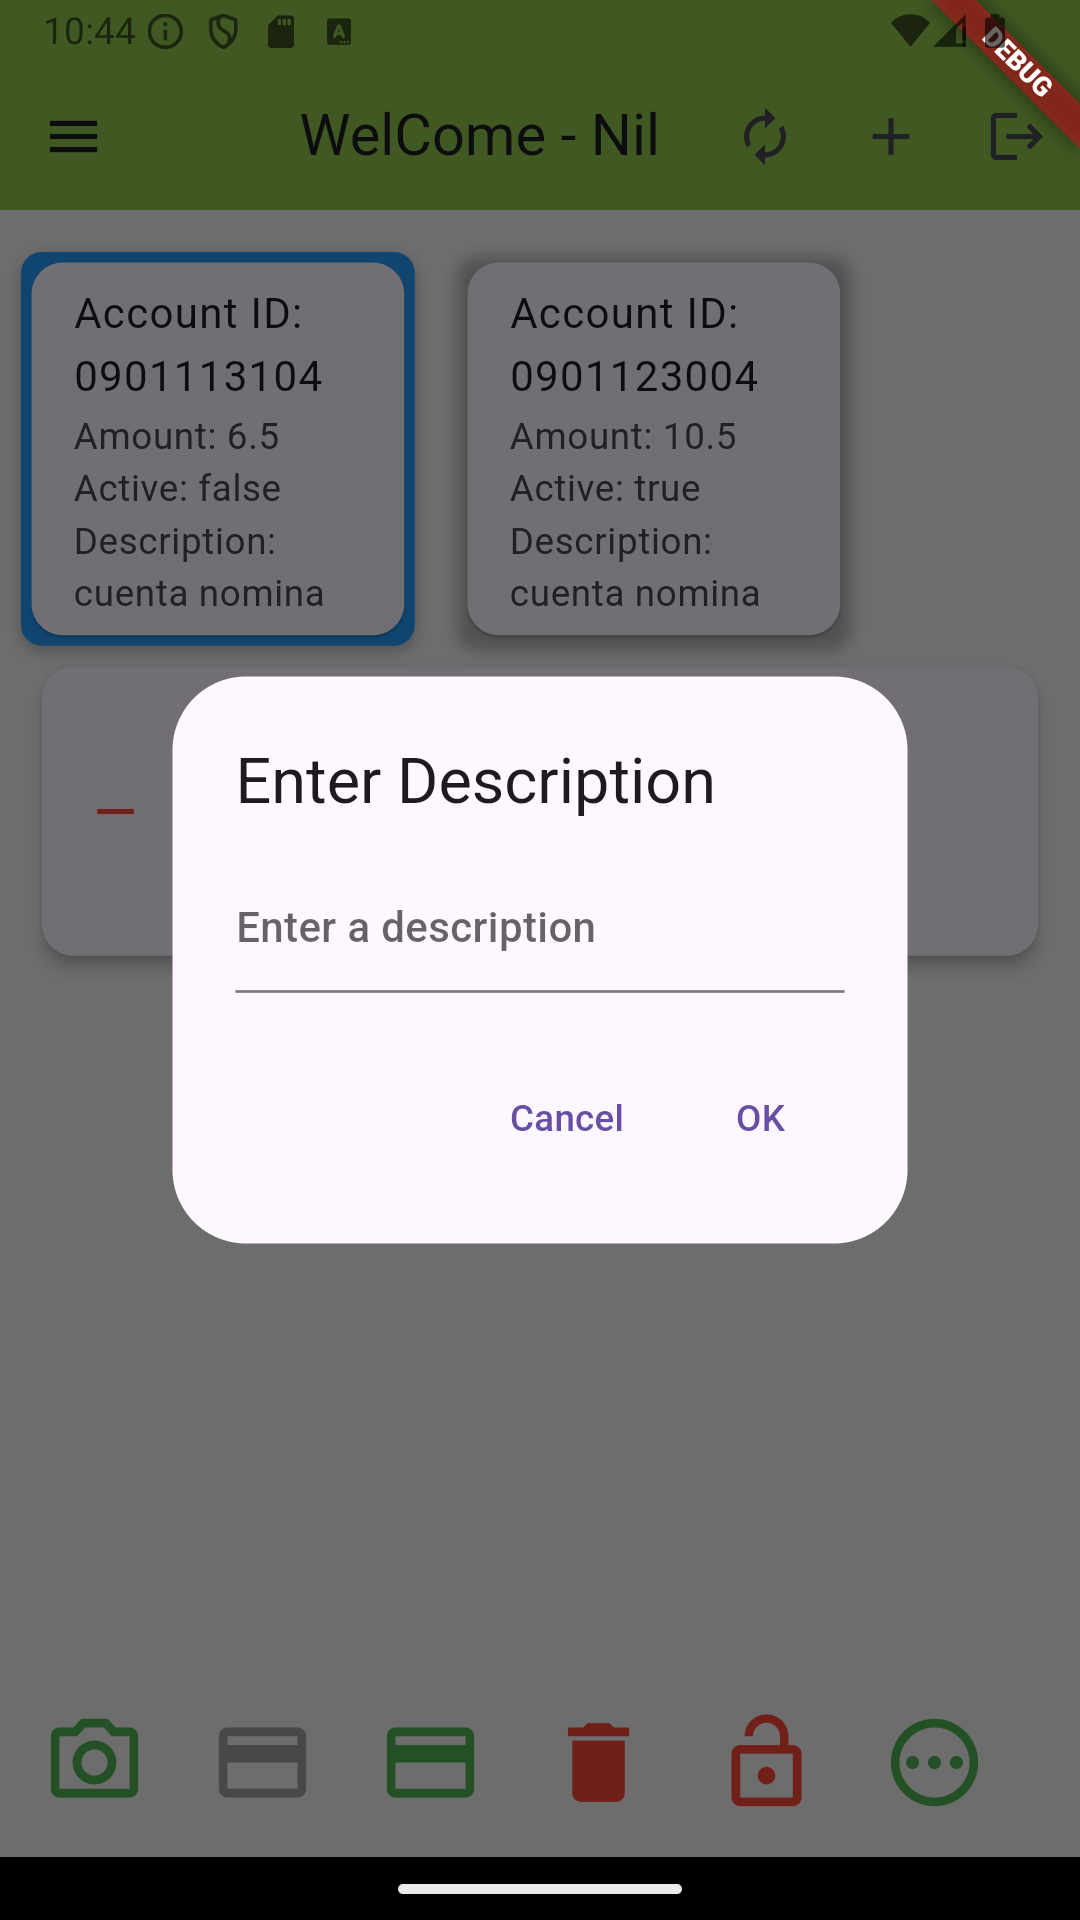
\includegraphics[width=\textwidth]{imatges/otherOperation3.png}
    \end{minipage}

    \caption{Modificar l'estat del compte bancari}
    \label{fig:Altres operacions sobre el compte bancari}
\end{figure}


\clearpage
\subsubsection{Afegir un compte bancari per a l'usuari}
\label{subsubsec:Afegir un compte bancari per a l'usuari}

Per afegir un nou compte bancari per a l'usuari, només cal clicar a l'icona de "+". Es generarà i es mostrarà el nou compte creat, amb un import per defecte de 10,50 €.

\begin{figure}[h]
    \centering
    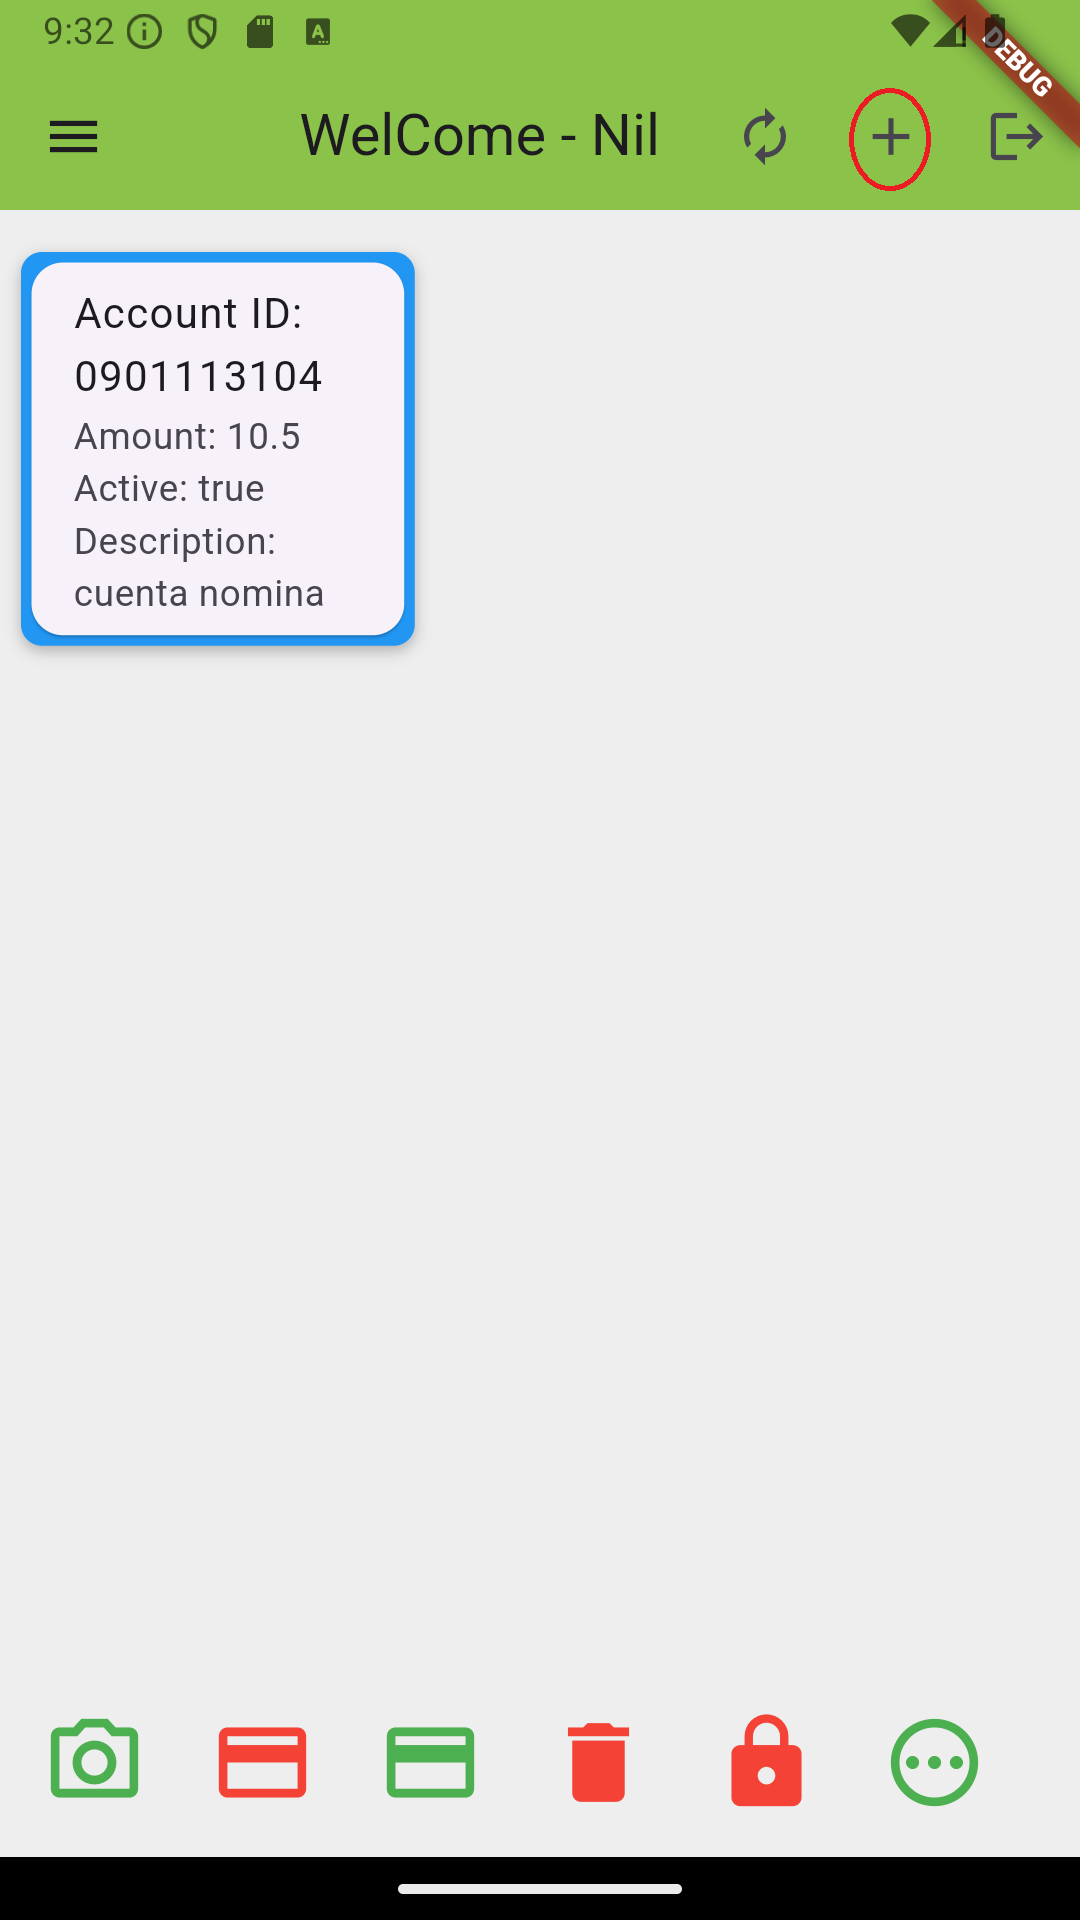
\includegraphics[width=0.4\textwidth]{imatges/mainpageAccount8.png}
    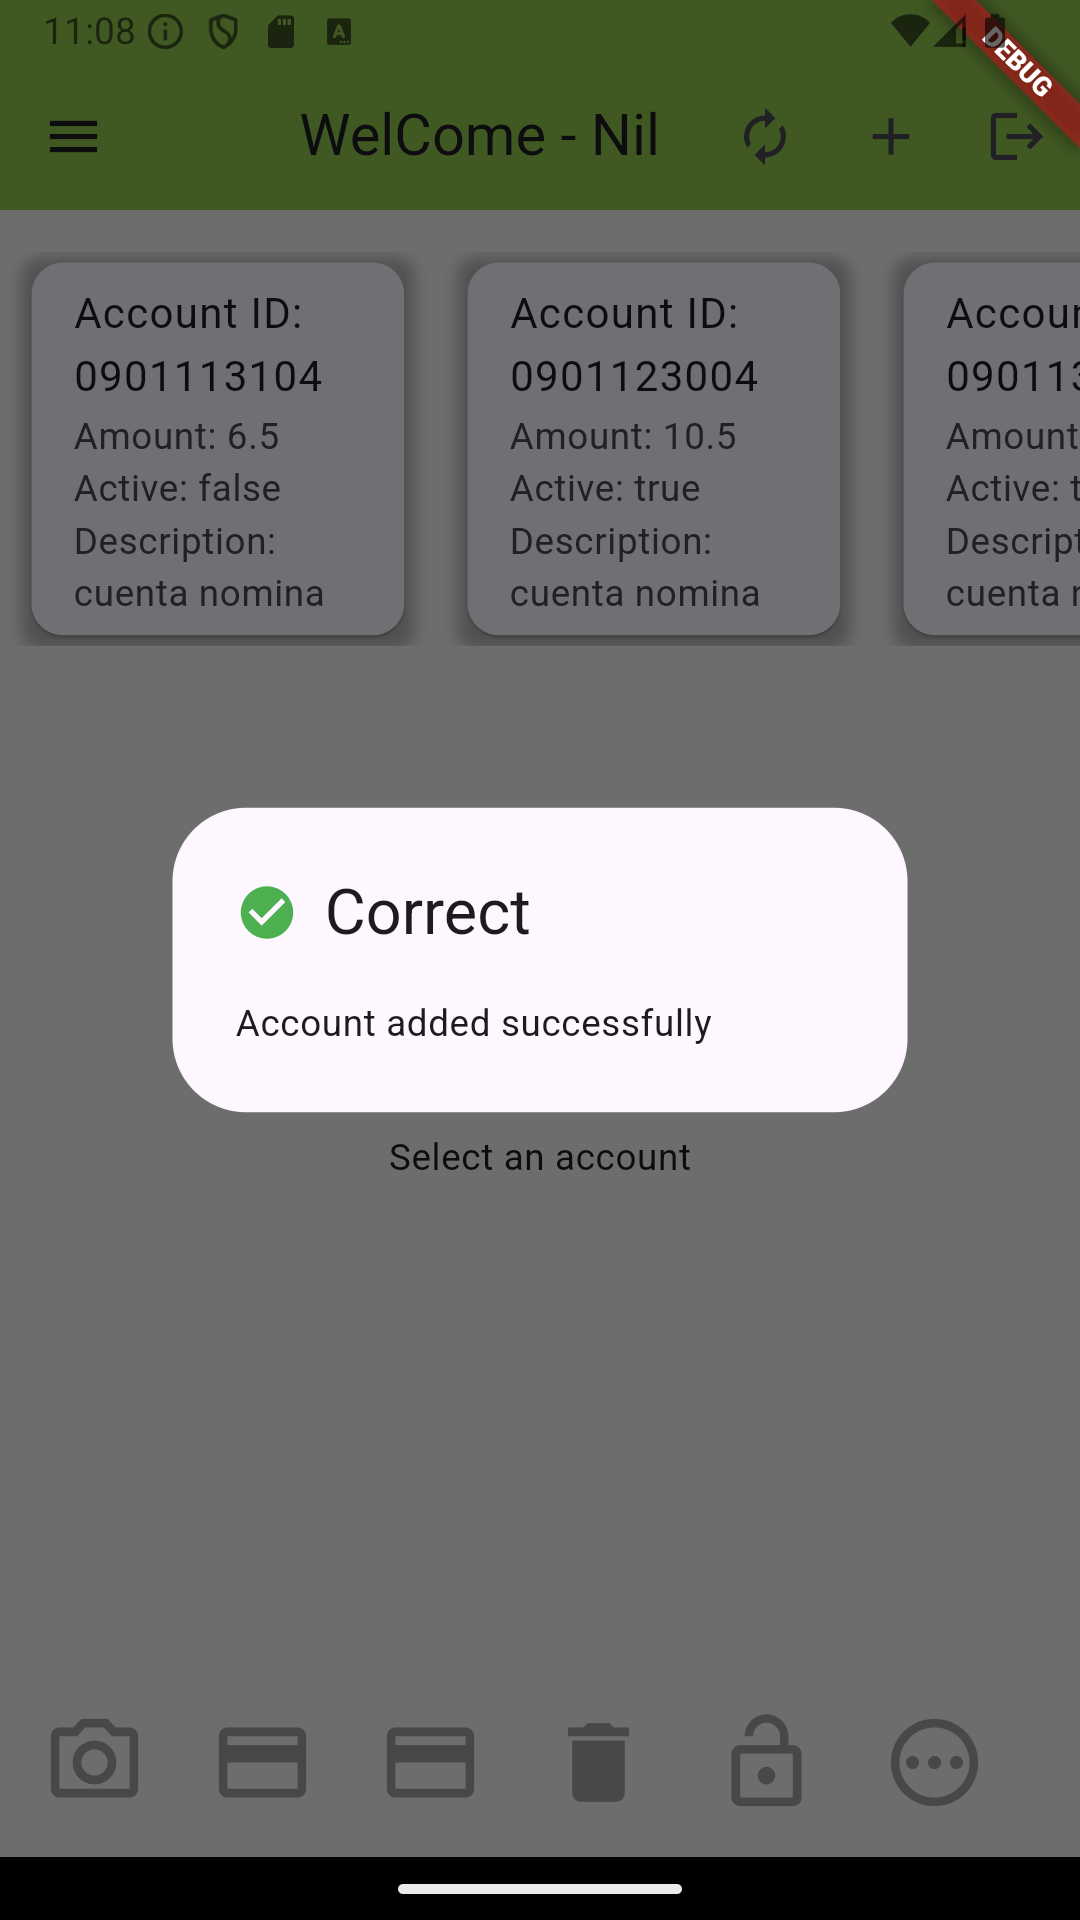
\includegraphics[width=0.4\textwidth]{imatges/addAccount.png}
    \caption{Afegir un compte bancari per a l'usuari}
    \label{fig: Afegir un compte bancari per a l'usuari}
\end{figure}


\clearpage
\subsubsection{Refrescar la pàgina}
\label{subsubsec:Refrescar la pàgina}

Per refrescar la pàgina, simplement clica al botó de refrescar. Això actualitzarà el contingut i mostrarà qualsevol canvi recent.

\begin{figure}[h]
    \centering
    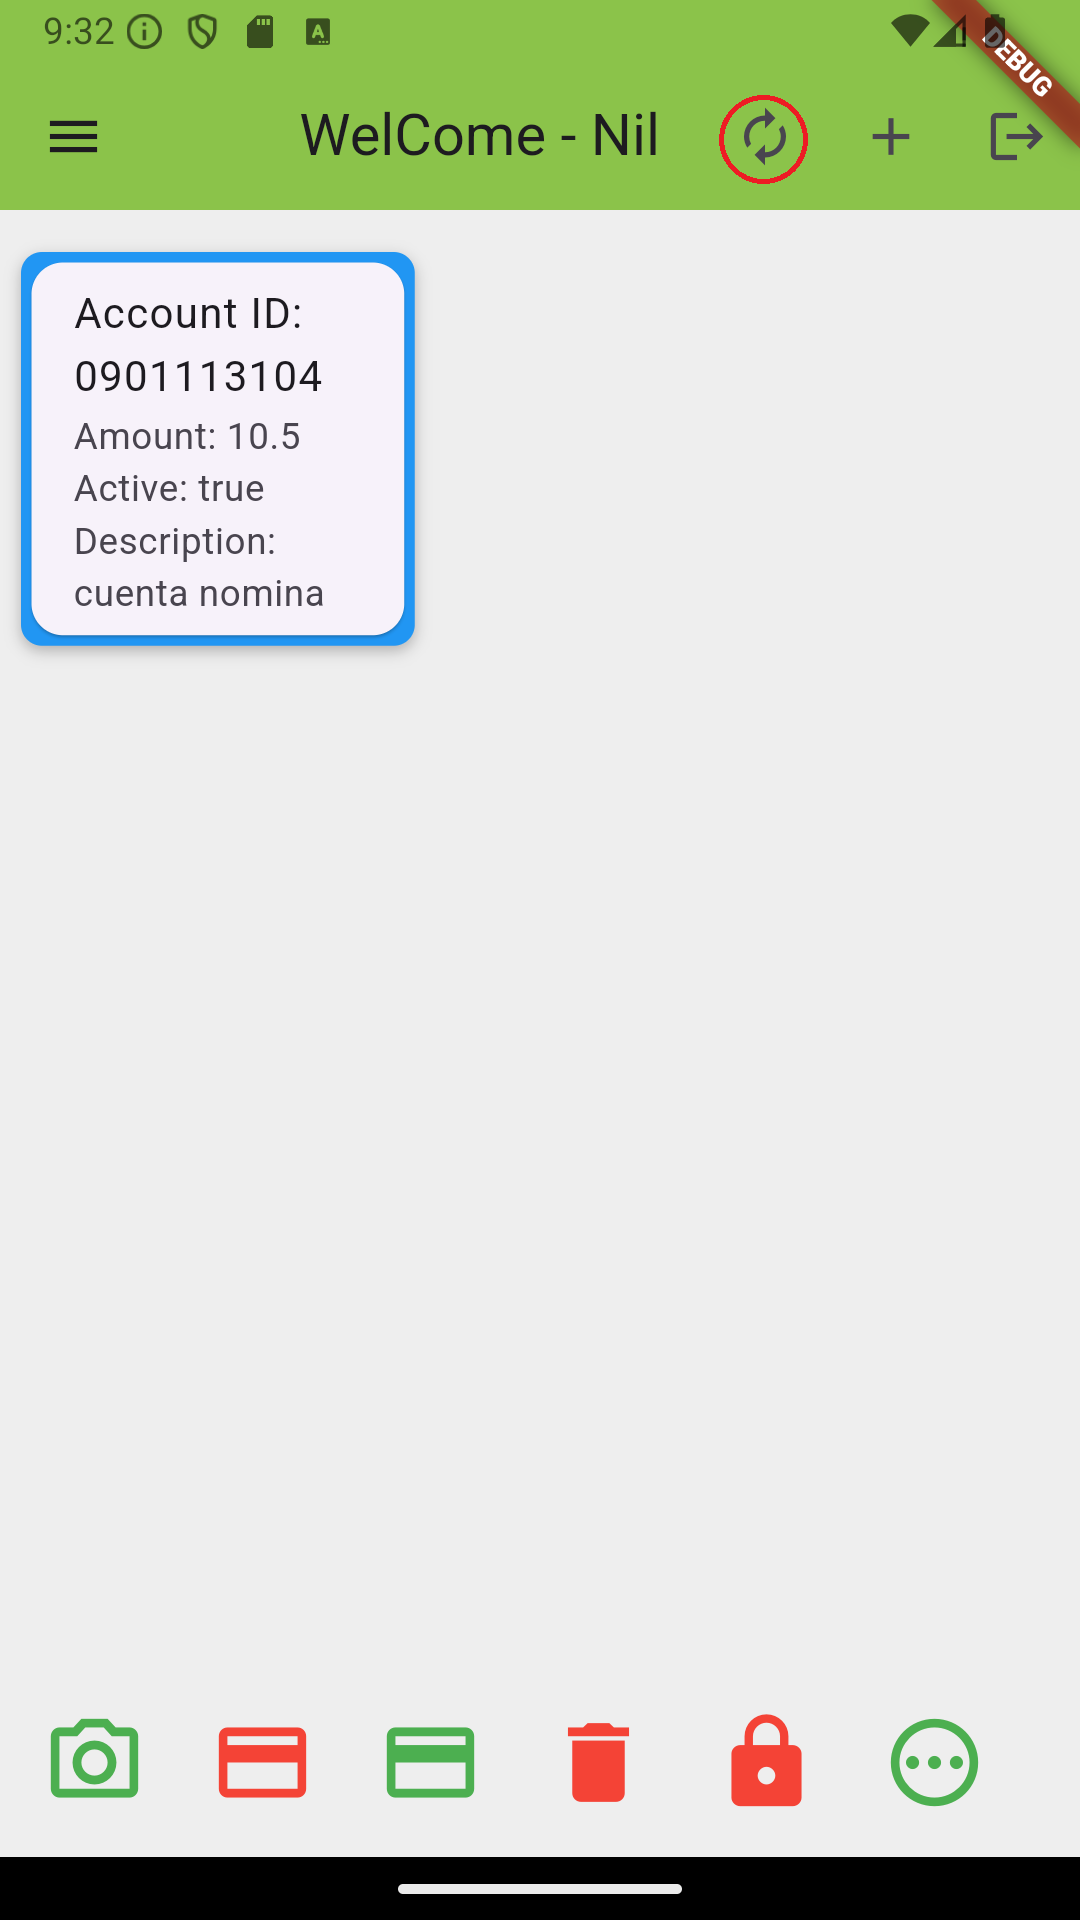
\includegraphics[width=0.4\textwidth]{imatges/mainpageAccount7.png}
    \caption{Refrescar la pàgina}
    \label{fig:Refrescar la pàgina}
\end{figure}

\clearpage
\subsubsection{Sortir de la secció}
\label{subsubsec:Sortir de la secció}

Per sortir de la secció, se't preguntarà si estàs segur que vols sortir. Un cop confirmada la teva decisió, es eliminaran les credencials i seràs redirigit a la pàgina de login.

\begin{figure}[h]
    \centering
    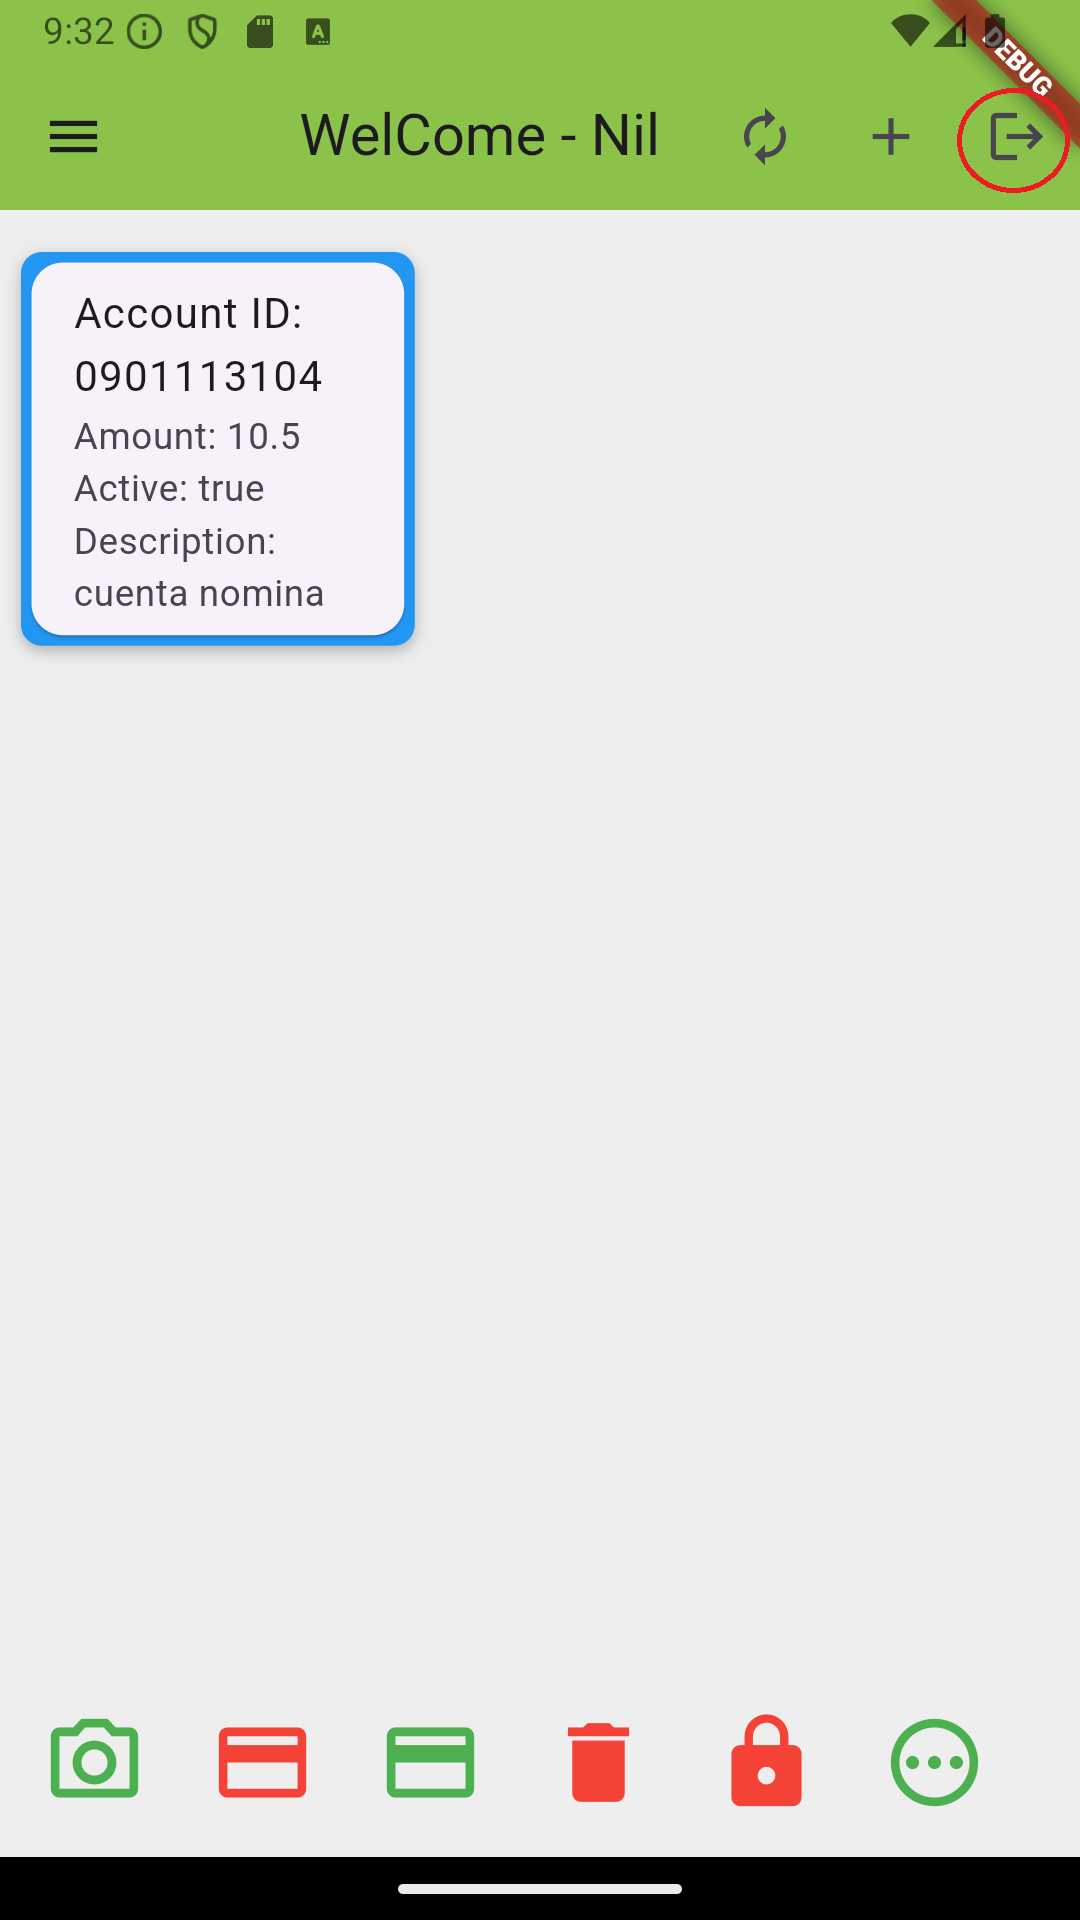
\includegraphics[width=0.31\textwidth]{imatges/mainpageAccount9.png}
    \includegraphics[width=0.31\textwidth]{imatges/logOut.png}
    \includegraphics[width=0.31\textwidth]{imatges/login.png}
    \caption{Sortir de la secció}
    \label{fig: Sortir de la secció}
\end{figure}

\clearpage

\subsubsection{Altres gestions de l'usuari}
\label{subsubsec:Gestió de l'usuari}

\begin{itemize}
    \item \textbf{Change password:} Per canviar la contrasenya, cal que introdueixis la contrasenya antiga i la nova dues vegades.
    \item \textbf{Change color:} Per canviar el color de fons, cal que seleccionis el color que més et conveni.
    \item \textbf{Set user status:} Per modificar l'estat de l'usuari, si l'usuari està desactivat no podrà realitzar cap operació amb el compte bancari.
    \item \textbf{Remove user:} Per eliminar l'usuari, cal que no hi hagi import en els seus comptes bancaris.
\end{itemize}

\begin{figure}[h]
    \centering
    \includegraphics[width=0.25\textwidth]{imatges/userGestion.png}
    \includegraphics[width=0.25\textwidth]{imatges/userGestion1.png}
    \includegraphics[width=0.25\textwidth]{imatges/userGestion3.png}
    \includegraphics[width=0.25\textwidth]{imatges/userGestion2.png}
    \includegraphics[width=0.25\textwidth]{imatges/userGestion4.png}
    \includegraphics[width=0.25\textwidth]{imatges/userGestion5.png}
    \caption{Altres gestions de l'usuari}
    \label{fig: Altres gestions de l'usuari}
\end{figure}



\clearpage
\subsection{Administrador}
\label{subsec: Admin}

L'usuari administrador és qui té permisos especials per gestionar i configurar l'aplicació, incloent la creació i eliminació d'altres usuaris, així com la gestió de configuracions i opcions avançades.

\subsubsection{Login d'un administrador}
\label{subsubsec: Login d'un administrador}

Un administrador accedeix de la mateixa manera que un client. Per defecte, hi ha un administrador predefinit amb el nom d'usuari \textit{"Admin"} i la contrasenya \textit{"Admin123"}. Aquest administrador no es pot eliminar. A partir d'aquí, es poden registrar altres administradors.

\begin{figure}[h]
    \centering
    \includegraphics[width=0.31\textwidth]{imatges/login.png}
    \includegraphics[width=0.31\textwidth]{imatges/loginAdmin.png}
    \includegraphics[width=0.31\textwidth]{imatges/administer.png}
    \caption{Pàgina de \textit{login} - Administrador}
    \label{fig: Pàgina de login - Admin}
\end{figure}



\clearpage
\subsubsection{Llistar els comptes de l'usuari i modificar l'estat del compte}
\label{subsubsec:Llistar els comptes de l'usuari i modificar l'estat del compte}

Un administrador permet visualitzar tots els usuaris clients i els seus comptes bancaris. També permet modificar l'estat dels comptes bancaris.

\begin{figure}[h]
    \centering
    \includegraphics[width=0.31\textwidth]{imatges/mainAdmin1.png}
    \includegraphics[width=0.31\textwidth]{imatges/userAccounts1.png}
    \includegraphics[width=0.31\textwidth]{imatges/userAccounts2.png}
    \caption{Llistar els comptes de l'usuari i modificar l'estat del compte}
    \label{fig: Llistar els comptes de l'usuari i modificar l'estat del compte}
\end{figure}



\clearpage
\subsubsection{Crear una nova contrasenya per client}
\label{subsubsec: Crear una nova contrasenya per client}

Un administrador pot canviar la contrasenya d'un usuari client sense haver de proporcionar la contrasenya antiga.\\

Cal proporcionar una contrasenya d'almenys 3 caràcters, i el canvi es pot efectuar només si les dues contrasenyes coincideixen.

\begin{figure}[h]
    \centering
    \includegraphics[width=0.31\textwidth]{imatges/mainAdmin2.png}
    \includegraphics[width=0.31\textwidth]{imatges/setPassword2.png}
    \includegraphics[width=0.31\textwidth]{imatges/setPassword3.png}
    \caption{Crear una nova contrasenya per client}
    \label{fig: Crear una nova contrasenya per client}
\end{figure}


\clearpage
\subsubsection{Modificar l'estat de l'usuari client}
\label{subsubsec: Modificar l'estat de l'usuari client}

Un administrador té el privilegi de modificar l'estat d'un usuari. Si un usuari té l'estat desactivat, no podrà realitzar cap operació sobre els comptes bancaris.

\begin{figure}[h]
    \centering
    \includegraphics[width=0.31\textwidth]{imatges/mainAdmin3.png}
    \includegraphics[width=0.31\textwidth]{imatges/confirmation.png}
    \includegraphics[width=0.31\textwidth]{imatges/confirmacion1.png}
    \caption{Modificar l'estat de l'usuari client}
    \label{fig: Modificar l'estat de l'usuari client}
\end{figure}


\clearpage
\subsubsection{Eliminar un usuari client}
\label{subsubsec: Eliminar un usuari client}

Només es pot eliminar un usuari client quan no hi hagi saldo en els seus comptes. Primer es fa una comprovació, i després es mostra un diàleg de confirmació.

\sudan{tornar a fer el codi, crear una nova funcio que es digui, removable}

\begin{figure}[h]
    \centering
    \includegraphics[width=0.4\textwidth]{imatges/mainAdmin4.png}
    \includegraphics[width=0.4\textwidth]{imatges/delete1.png}
    \caption{Eliminar un usuari client}
    \label{fig: Eliminar un usuari client}
\end{figure}



\clearpage
\subsubsection{Visualitzar els moviments d'un usuari}
\label{subsubsec: Visualitzar els moviments d'un usuari}


Un administrador visualitzar tots els moviments de tots els usuari clients.

\begin{figure}[h]
    \centering
    \includegraphics[width=0.4\textwidth]{imatges/mainAdmin5.png}
    \includegraphics[width=0.4\textwidth]{imatges/movements.png}
    \caption{Visualitzar els moviments d'un usuari}
    \label{fig: Visualitzar els moviments d'un usuari}
\end{figure}



\clearpage
\subsubsection{Llistar tots els administradors i veure els seus moviments}
\label{subsubsec: Llistar tots els administradors i veure els seus moviments}

Els administradors poden veure les operacions realitzades entre ells.


\begin{figure}[h]
    \centering
    % Primera fila de dos imatges
    \begin{minipage}{0.31\textwidth}
        \includegraphics[width=\linewidth]{imatges/adminMain.png}
        \includegraphics[width=\linewidth]{imatges/showAdminMovement.png}
    \end{minipage}
    % Segona fila de tres imatges
    \begin{minipage}{0.31\textwidth}
        \includegraphics[width=\linewidth]{imatges/adminNavigation1.png}
        \includegraphics[width=\linewidth]{imatges/showHisMovements.png}
    \end{minipage}
    
    \caption{Llistar tots els administradors i veure els seus moviments}
    \label{fig:Llistar tots els administradors i veure els seus moviments}
\end{figure}




\clearpage
\subsubsection{Canviar la pròpia contrasenya}
\label{subsubsec: Canviar la pròpia contrasenya}

L'usuari administrador pot modificar la seva pròpia contrasenya, però cal introduir la contrasenya antiga.

\begin{figure}[h]
    \centering
    \includegraphics[width=0.31\textwidth]{imatges/adminMain.png}
    \includegraphics[width=0.31\textwidth]{imatges/adminNavigation2.png}
    \includegraphics[width=0.31\textwidth]{imatges/adminchangepassword.png}
    \caption{Canviar la pròpia contrasenya}
    \label{fig:Canviar la pròpia contrasenya }
\end{figure}




\chapter{Implementació i proves}
\label{chp:implementacio}


\section{Introducció}
\label{sec: Introducció}

L'objectiu d'aquest capítol és explicar el procés de desenvolupament, des de la idea inicial de l'aplicació i la seva estructura fins al desenvolupament actual de la mateixa. També s'inclourà una explicació sobre com s'ha provat constantment l'aplicació. A més, es detallaran les diferents proves que s’han realitzat per verificar el funcionament de l’aplicació.\pau{(potser millor ``També s'explicaran les diferents proves que s'han dut a terme per verificar el funcionament de l'aplicació'')}.\sudan{corregit}


\section{Idea inicial \pau{(potser millor ``Idea inicial'')}}\sudan{corregit}
\label{sec: Organitza la idea}

Quan se'm va ocórrer la idea de l'aplicació, vaig acabar amb una barreja de pensaments i conceptes que necessitaven ser organitzats i connectats de manera coherent. El primer pas en aquest procés va ser redactar una explicació detallada de l'aplicació, incloent l'objectiu general, les funcionalitats principals que hauria d'oferir, així com les limitacions i allò que no inclouria. Va ser essencial intentar cobrir tants detalls com fos possible per assegurar una comprensió clara del projecte.\\

Durant aquesta fase, vaig analitzar com es relacionava cada component de l'aplicació amb els altres i com s'integraria dins del sistema global. Vaig considerar les possibles interaccions entre les diferents funcionalitats i com aquestes podrien impactar en l'experiència de l'usuari. A més, vaig revisar diversos enfocaments arquitectònics per determinar el més adequat per aconseguir els objectius establerts.\\

Tot i que probablement canviaria l'estructura en el futur en resposta a noves necessitats o oportunitats de millora, la idea inicial de l'arquitectura va ser útil per establir una base sòlida. A partir d'aquesta base, vaig poder començar a especificar els requisits funcionals i no funcionals de manera més detallada. Aquesta etapa va ser probablement la tasca més exigent del projecte, ja que va requerir una atenció meticulosa a cada aspecte del disseny i l'estructura, a més de l'organització dels paquets de treball. Després que aquestes parts estiguessin definides i estructurades, vaig poder visualitzar un full de ruta clar i detallat per al desenvolupament del sistema, el que em va permetre avançar amb una estratègia ben definida i metòdica.



\section{Biblioteques utilitzades}
\label{sec: Biblioteques utilitzades}


Per a aquest projecte, ha estat necessari utilitzar diverses biblioteques que han facilitat el desenvolupament i la implementació de les funcionalitats previstes. Aquestes biblioteques han proporcionat les eines i els recursos necessaris per gestionar diferents aspectes del projecte.\\

A continuació, es detallen les biblioteques específiques que s'han utilitzat i la seva utilitat en el context del projecte, com ara generar codis QR, llegir codis QR, encriptar missatges, gestionar contrasenyes i administrar credencials.




\subsection{Generar codi QR}
\label{subsec: Generar codi QR}

Per generar codis QR en Flutter, una biblioteca popular és \textbf{qr\_flutter}. Aquesta biblioteca facilita la creació de codis QR a partir de text i la seva renderització com a widgets dins de l'aplicació Flutter. A més de la seva funcionalitat bàsica, qr\_flutter ofereix diverses opcions de personalització, com ara ajustar la mida del codi QR, configurar el color del codi QR i afegir imatges al centre del codi QR.\\

El problema que vaig trobar en la generació del codi QR es deu a l'actualització de la biblioteca qr\_flutter. En les versions \textit{2.0.0} fins a a \textit{3.0.0}, utilitzàvem la nomenclatura \textit{QrImage}. No obstant això, en la versió actual \textit{4.1.0}, s'ha actualitzat a \textit{QrImageView}. Inicialment, això causava errors de compilació perquè el sistema no reconeixia \textit{QrImage}. Em va sorprendre molt, però finalment vaig descobrir que el problema es devia a aquesta actualització.\\ 

En la figura~\ref{fig:Versió antiga vs. versió nova}  es mostren dues imatges que il·lustren el codi per a les dues versions:

\begin{figure}[h]
    \centering
    \includegraphics[width=0.5\textwidth]{imatges/qrold.png}
    \includegraphics[width=0.5\textwidth]{imatges/qrnew.png}
    \caption{Versió antiga vs. versió nova}
    \label{fig:Versió antiga vs. versió nova}
\end{figure}


\clearpage
\subsection{Llegir codi QR}
\label{subsec: Llegir codi QR}

Per llegir codis QR en Flutter, aquest projecte utilitza la biblioteca \textbf{qr\_code\_scanner}. Aquesta biblioteca facilita la lectura de codis QR mitjançant la càmera del dispositiu i permet integrar fàcilment la funcionalitat d'escanneig de codis QR en aplicacions Flutter. Ofereix una solució senzilla i eficient per capturar i processar dades codificades en codis QR.\\

Vaig trobar un problema, encara que vaig sortir de la pantalla de la càmera, el webcam del portàtil seguia encès. La solució consisteix a utilitzar el controlador de la biblioteca \textbf{qr\_code\_scanner}. Cal controlar el controlador de la càmera i assegurar-se de cridar el mètode \textit{dispose()} quan ja no es necessiti utilitzar la càmera.


\subsection{Encriptar Missatge}
\label{subsec: Encriptar Missatge}

Per encriptar els missatges dels codis QR en flutter, utilitza la biblioteca \textbf{encrypt 5.0.3}. Aquesta biblioteca ofereix una àmplia gamma de mètodes d'encriptació, i per a aquesta pràctica s'ha escollit l'algorisme AES.\\

La biblioteca encrypt proporciona eines robustes per gestionar tant l'encriptació com la desencriptació de dades, facilitant així la protecció de la informació codificada en els codis QR. L'algorisme AES (Advanced Encryption Standard) és un mètode de xifrat simètric que utilitza la mateixa clau per a l'encriptació i la desencriptació, garantint així la seguretat de les dades. Utilitzant AES, podem assegurar que els missatges emmagatzemats en els codis QR siguin segurs i només accessibles per aquells que disposin de la clau correcta per desencriptar-los.\\

Inicialment, vaig implementar una clau única per a tots els usuaris de l'aplicació. No obstant això, vaig adonar-me que aquesta solució podia ser molt arriscada en cas de pèrdua de la clau. Per garantir la màxima seguretat, he optat per utilitzar una clau independent per a cada compte bancari. A més, a mesura que es generen nous codis QR de pagament, la clau associada s'actualitza automàticament.


\subsection{Encriptar la contrasenya}
\label{subsec: Encriptar la contrasenya}

Per guardar les contrasenyes dels usuaris a la base de dades, és molt perillós emmagatzemar-les en text clar. Per garantir la seguretat, aquest projecte utilitza la biblioteca crypto de Node.js. El mòdul crypto de Node.js proporciona eines essencials per a la seguretat de les aplicacions, incloent funcionalitats com encriptació, hashing, signatura digital i més. En aquest projecte, s'empla la funcionalitat de hashing.\\

El hashing és una tècnica criptogràfica clau que transforma les dades en una representació fixa i, idealment, irreversible. Aquesta tècnica permet emmagatzemar les contrasenyes de manera segura, verificar la integritat de les dades i assegurar l'autenticitat dels missatges gràcies a les seves propietats úniques.


\subsection{Gestionar les credencials}
\label{subsec: Gestionar les credencials}


En aquest projecte, gestionem les credencials d'usuari utilitzant la biblioteca jsonwebtoken. Aquesta biblioteca proporciona les eines necessàries per treballar amb tokens JWT, que són essencials per a l'autenticació i l'autorització d'usuaris. Les funcions inclouen:

\begin{itemize}
    \item \textbf{Generació de Tokens d'Accés}: La funció getAccessToken crea un token JWT signat amb una clau secreta a partir d'un payload proporcionat. Aquest token es configura amb una durada de 1 dia, la qual cosa significa que l'usuari haurà de tornar a autenticar-se després d'aquest període per obtenir un nou token.
    \item \textbf{Verificació de Tokens}: La funció getUserId extreu i verifica el token JWT des de l'encapçalament d'autorització de la sol·licitud. Si el token és vàlid, retorna l'identificador de l'usuari emmagatzemat en el token, permetent accedir a recursos protegits.
\end{itemize}


\pau{Aquí es podria explicar també les biblioteques que ha calgut utilitzar per generar i llegir codis QR, com les has integrat a la teva aplicació, problemes que t'has trobat i com els has solucionat, etc. I el mateix per biblioteques o mòduls utilitzats per encriptar missatges.}


\section{Desenvolupament d'aplicació}
\label{sec: desenvolupament d'aplicació }

Vaig començar a desenvolupar el servidor \pau{(vols dir l'API de l'aplicació?)}\sudan{corregit}, ja que això ajudava a definir la base de dades. La meva estratègia consistia a implementar primer les funcionalitats més crítiques i bàsiques, assegurant-me que cada component essencial funcionés correctament abans de passar a les següents etapes. Per exemple, vaig començar amb l'operació de transacció entre dos comptes bancaris, assegurant-me que aquest procés fonamental fos fiable. Un cop aquesta funcionalitat va estar operativa, vaig afegir seguretat amb l'encriptació de dades. Posteriorment, vaig implementar controls addicionals, com ara verificar si un compte disposava de saldo suficient i comprovar si el compte estava actiu.\\

Un cop vaig tenir una base sòlida al servidor, vaig començar a dissenyar la interfície d'usuari. Durant aquest procés, vaig adaptar el disseny en funció dels punts finals disponibles i les funcionalitats implementades en el servidor, mentre identificava les possibles mancances en l'API. Així, després de completar el disseny de la interfície, vaig tornar a l'API per afegir les funcionalitats que faltaven i per netejar el codi existent.\\

A mesura que avançava en el desenvolupament, vaig començar a treballar en les interfície d'usuari \pau{(potser millor ``vaig començar a treballar en les interfícies d'usuari'')}\sudan{corregit}. Vaig desenvolupar primer l'aplicació bàsica \pau{(aplicació?)}, que contenia la major part de la lògica i complexitat. Aquesta fase va ser crucial, ja que vaig afegir diversos components i vistes que posteriorment es reutilitzarien a l'aplicació client. Vaig adoptar un enfocament iteratiu: cada vegada que afegia o ajustava una funcionalitat en el servidor, feia el mateix en el client, variant les funcionalitats de manera sincronitzada. Aquesta estratègia em va permetre assegurar-me que ambdues parts de l'aplicació estiguessin alineades i funcionessin conjuntament.\\

Tot i que no vaig utilitzar eines específiques com ``Nx'', vaig intentar fer abstracció i reutilitzar el codi de manera eficaç per simplificar el desenvolupament. Si en el futur es necessita afegir un altre projecte \pau{(aplicació?)}\sudan{corregit}, el procés serà més senzill, ja que molts components i funcions podrien ser reutilitzats.


\section{Problemes i Solucions en la Implementació}
\label{sec:Problemes i Solucions en la Implementació}

Durant el desenvolupament del projecte, s'han presentat diversos reptes i obstacles que han afectat la implementació de les funcionalitats previstes. A mesura que avançava en el procés, vaig identificar diversos problemes que requereixen una atenció detallada per garantir el bon funcionament de l'aplicació.\\

En aquest apartat, es descriuen els problemes més significatius que vaig trobar, juntament amb les estratègies i solucions que vaig aplicar per superar-los. Cada problema s'explica en detall, incloent el context en què va sorgir, l'impacte que va tenir sobre el projecte, i les solucions implementades per resoldre'l. Aquest enfocament proporciona una visió clara dels desafiaments afrontats i de com es va assegurar el bon desenvolupament i la funcionalitat final del projecte.\\


\subsection{Android Studio}
\label{subsec: Android Studio}

Vaig enfrontar diversos problemes amb Android Studio. Amb el mateix codi, l'aplicació fallava al dia següent. Inicialment, no estava clar si el problema es devia a Android Studio o al codi mateix. Vaig intentar revisar les versions anteriors del codi utilitzant el control de versions, però això no va resoldre el problema.\\

En la figura~\ref{fig:Problemes d'implementació amb Android Studio} es mostra un dels errors que he trobat.

\begin{figure}[h]
    \centering
    \includegraphics[width=1\textwidth]{imatges/errorAndroid.png}
    \caption{Problemes d'implementació amb Android Studio}
    \label{fig:Problemes d'implementació amb Android Studio}
\end{figure}

Més endavant, vaig descobrir que el simulador sovint es pot omplir de memòria, cosa que pot provocar que no arranqui correctament. El simulador té un límit de memòria, i gestionar-ho adequadament és important per garantir que funcioni de manera fluida. Si experimentes problemes de rendiment, cal ajustar la configuració del simulador i fer una neteja periòdica de dades. La solució que faig servir és realitzar un \textbf{wipe data} del simulador, el qual neteja les dades emmagatzemades i resol els problemes de càrrega.\\


Una altra opció que es pot combinar amb el wipe data és crear una pàgina d'entrada simple. Aquesta mesura permet comprovar si el problema es resol amb un simulador net, abans de tornar a implementar el codi del projecte. D'aquesta manera, es pot excloure la possibilitat que el problema provingui del codi i determinar si el problema és del simulador. Un altre avantatge d'aquesta pàgina simple és que permet fer implementacions complexes en aquest espai de manera independent del codi global, cosa que facilita les proves en casos quan no es té la seguretat total sobre la funcionalitat.\\

La figura~\ref{fig: pàgina de prova} mostrada a continuació presenta el codi de la pàgina simple (mutation.dart). Aquesta pàgina es carrega canviant la ruta del main.

\begin{figure}[h]
    \centering
    \includegraphics[width=1\textwidth]{imatges/hola.png}
    \caption{Pàgina de prova}
    \label{fig: pàgina de prova}
\end{figure}

\subsection{Flutter}
\label{subsec: Flutter}

Si l'error de compilació no es pot resoldre amb les mesures esmentades anteriorment, és probable que el problema estigui relacionat amb el compilador de Flutter.\\

La comanda \textbf{flutter clean} és utilitzat per netejar el directori de construcció i altres fitxers generats que poden causar problemes. Posteriorment cal fer servir \textbf{flutter pub get} per tornat a descarregar les dependències. Algunes situacions en què és necessari utilitzar aquesta comanda inclouen:

\begin{itemize}
  \item Problemes de Compilació
  \item Actualitzacions de Dependències
  \item Problemes Amb el Simulador o Dispositiu
  \item Actualització de Flutter o el SDK
\end{itemize}

També hi ha la comanda \textbf{flutter doctor}, que és utilitzat per verificar la configuració de l'entorn de desenvolupament i solucionar problemes de configuració. Algunes situacions en què és necessari utilitzar aquesta comanda inclouen:

\begin{itemize}
  \item Verificació de l'Entorn de Desenvolupament
  \item Solució de Problemes de Configuració
  \item Abans de Reportar Problemes 
\end{itemize}

Aquesta imatge~\ref{fig: Comanda flutter doctor} mostra l'execució de flutter doctor, indicant que l'entorn de desenvolupament està configurat correctament.
\begin{figure}[h]
    \centering
    \includegraphics[width=1\textwidth]{imatges/flutterdoctor.png}
    \caption{Comanda flutter doctor}
    \label{fig: Comanda flutter doctor}
\end{figure}


\subsection{GitHub}
\label{subsec: GitHub}

Un error important que vaig cometre en aquest projecte va ser que, quan el codi no arrencava, la primera cosa que feia era anar al repositori i retirar els commits, fent còpies del projecte localment per seguretat. Si, després de retirar un commit, el codi seguia sense funcionar, procedia a retirar-ne un altre, i així successivament.\\

Més endavant, em vaig adonar que aquest enfocament no era efectiu i em vaig adonar que "això no és possible; el codi de fa una setmana funcionava correctament..."\\

En aquest punt, em vaig adonar que la millor solució era recuperar els commits, però sovint em trobava bloquejat, ja que havia eliminat commits del repositori local sense sincronitzar-los amb el repositori remot. Això em va portar a perdre temps i a confondre'm en diverses ocasions.\\

Per solucionar aquest problema, és necessari estudiar a fons les comandes de Git:


\subsubsection{Eliminar Commits}

\begin{itemize}
    \item \textit{git reset --soft HEAD~1}: Elimina el commit més recent però manté els canvis en l'índex.
    \item \textit{git reset --hard HEAD~1}: Elimina el commit més recent i descarta els canvis.
    \item \textit{git revert <commit>}: Desfà els canvis d'un commit específic creant un nou commit que els elimina.
    \item \textit{git rebase -i HEAD~n}: Permet modificar, combinar o eliminar múltiples commits en l'historial.
  \end{itemize}

\subsubsection{Recuperar Commits}

\begin{itemize}
  \item \textit{git log}: Mostra l'historial de commits i identifica el commit que vols recuperar.
  \item \textit{git checkout <commit>}: Permet revisar l'estat de l'arbre de treball en el moment d'un commit específic.
  \item \textit{git cherry-pick <commit>}: Aplica els canvis d'un commit específic a la branca actual.
  \item \textit{git reflog}: Mostra l'historial de referències i permet recuperar commits que no són visibles en l'historial normal.
\end{itemize}


\subsection{MongoDB}
\label{subsec: MongoDB}

Vaig passar més d'un dia barallant-me amb un error aparentment simple. El problema era el següent: tenia la taula \textbf{users} creada, però no contenia tots els atributs necessaris. Un dels atributs era el compte bancari, i volia actualitzar-lo per incloure una llista de comptes bancaris.\\

Vaig revisar tots els atributs de l'esquema i vaig revisar el codi del resolver una i altra vegada. Vaig anar a MongoDB per esborrar totes les dades anteriors de la taula (sense eliminar la taula mateixa). No hi havia manera que funcionés correctament; només es podia inserir un sol compte bancari, tot i que el servidor indicava que la inserció es realitzava correctament.\\

Finalment, vaig descobrir que havia d'eliminar la taula sencera per poder efectuar l'actualització, com indica la figura~\ref{fig: Eliminar la taula de mongoDB} següent.


\begin{figure}[h]
    \centering
    \includegraphics[width=1\textwidth]{imatges/eliminarMongo.png}
    \caption{Eliminar la taula de mongoDB}
    \label{fig: Eliminar la taula de mongoDB}
\end{figure}



\pau{Faltaria indicar quins problemes t'has trobat durant la implementació (sigui el que sigui), i com els has acabat solucionant.}\sudan{corregit}


\section{Proves}
\label{sec: Proves}

Aquesta secció descriu diverses categories de proves que es duen a terme durant el desenvolupament de programari per assegurar la seva qualitat i el correcte funcionament. A continuació es presenta un breu resum de cada tipus de prova:

\begin{itemize}
\item \textbf{Proves d'unitat}: Aquestes proves se centren en verificar el correcte funcionament de les parts més petites del codi, com funcions o mètodes, de manera independent.
\item \textbf{Proves d'integració}: L'objectiu d'aquestes proves és assegurar que les diferents unitats de codi treballin bé conjuntament quan es combinen, garantint així el bon funcionament del sistema en el seu conjunt.
\item \textbf{Proves de regressió}: Aquestes proves es realitzen per garantir que les noves funcionalitats o canvis no han introduït errors en altres parts del sistema. Es tornen a executar proves prèvies per assegurar que el comportament del sistema no ha canviat de manera inesperada.
\item \textbf{Proves de sistema}: Aquestes proves verifiquen que tot el sistema compleixi amb els requisits establerts, utilitzant escenaris d'ús que reflecteixen situacions reals.
\item \textbf{Proves d'acceptació de l'usuari}: Aquestes proves són realitzades per usuaris finals en un entorn que simula el real, per obtenir el seu \textit{feedback} sobre la usabilitat i l'adequació de les noves funcionalitats.
\item \textbf{Proves de càrrega i rendiment}: Es realitzen per avaluar com es comporta el sistema sota condicions de càrrega elevades i diferents situacions de rendiment, ajudant a identificar possibles problemes i millores necessàries.
\item \textbf{Proves de seguretat}: Aquestes proves tenen l'objectiu de verificar que el sistema és segur i està protegit contra vulnerabilitats i atacs potencials.
\item \textbf{Proves de compatibilitat}: S'utilitzen per assegurar que el sistema funcioni correctament en diverses plataformes, navegadors, dispositius i sistemes operatius.
\end{itemize}

L'aplicació de la interfície d'usuari (IU) s'ha provat manualment per trobar errors. En el cas de l'API, provar els punts finals ha estat una mica més difícil, però s'ha utilitzat programari especialitzat per fer-ho. Pel que fa a les aplicacions d'interfície d'usuari, s'han provat casos avançats executant l'aplicació. Quan s'ha trobat un error, primer he revisat les proves per veure si el cas no estava cobert o si va ser un error en la prova, ja que és una situació que pot passar. Si es trobava un error en les proves, actualitzava les proves i després corregia el codi real. Si no es trobava un error en les proves, buscava l'error en el codi i després el cobria amb les proves.

\pau{Seria interessant posar un exemple del teu propi projecte per cada tipus de proves llistat abans.}




\chapter{Implantació i resultats}
\label{chp:implantacio}


\section{Implantació}
\label{sec: Implantació}

La implantació de l'aplicació es realitza en diverses fases, amb un enfocament gradual per assegurar la qualitat i funcionalitat del sistema. La fase inicial del projecte va consistir en desenvolupar l'aplicació de pagament mitjançant codi QR. Aquesta primera etapa es va centrar en establir la infraestructura bàsica necessària per generar i escanejar codis QR associats a transaccions de pagament.\\

Un cop l'aplicació va estar operativa amb les funcionalitats bàsiques, la següent etapa va ser la incorporació d'una passarel·la de pagament. Aquesta passarel·la és crucial per processar les transaccions de pagament de manera segura i eficient. Actualment, el desenvolupament de la passarel·la està en curs, i la seva integració és el següent pas important per completar la implantació de l'aplicació.\\

El projecte té dues vies potencials per a la seva implantació futura. La primera opció és integrar l'aplicació amb els sistemes bancaris estatals, similar a com funciona Bizum. Aquesta integració permetria que l'aplicació ofereixi funcionalitats similars a les d'un servei de pagament a través de bancs. La segona opció és establir una passarel·la de pagament pròpia, creant una solució similar a PayPal que permeti operar com una empresa de pagaments independent. Aquesta opció ofereix una major autonomia i flexibilitat en la gestió de les transaccions.

\pau{També hauries de parlar de quines mesures has pres o prendries en el moment de la implantació pel que fa a garantir la protecció de dades (i, per tant, la legislació i normatives vigents).}


\section{Resultats}
\label{sec: Resultats}

Fins al moment, l'aplicació ha aconseguit implementar les funcionalitats bàsiques necessàries per generar i escanejar codis QR. No obstant això, encara falta integrar la passarel·la de pagament per completar el procés de pagament. La principal dificultat actual és la integració amb la passarel·la, que requereix una coordinació complexa amb els proveïdors de serveis de pagament i la implementació de mesures de seguretat addicionals.\\

Els beneficis esperats de l'aplicació són significatius. Un cop completada, l'aplicació permetrà als usuaris realitzar pagaments de manera senzilla i segura utilitzant codis QR, amb opcions tant per integrar-se amb bancs com per utilitzar una passarel·la de pagament pròpia. Aquesta flexibilitat en els mètodes de pagament oferirà una alternativa valuosa a serveis establerts com PayPal i proporcionarà als usuaris una solució innovadora i eficient per als seus pagaments.\\

Els pròxims passos en el desenvolupament inclouen la finalització de la integració de la passarel·la de pagament i la implementació de les funcionalitats avançades. A continuació, es realitzaran proves exhaustives per garantir el bon funcionament del sistema abans del llançament oficial de l'aplicació.

\pau{Tot això que has posat ja ho has mig explicat a la secció anterior i, en tot cas, seria més pertintent posar-ho a ``treball futur''. Aquí a resultats has de mostrar com ha quedat l'aplicació final, amb captures de les diferents pantalles, i explicant com cadascuna assoleix els objectius plantejats inicialment. Les captures han de ser les finals, mentre que al Capítol~\ref{chp:analisi} hi ha d'anar només el disseny inicial de les pantalles (esbossos).}

\pau{Tot això de les proves no hi ha d'anar! Ja les expliques al capítol anterior.}



% \section{Prova 1}
% \section{Prova 2}
% \section{Prova 3}
% \section{Prova 4}
% \section{Prova 5}
% \section{Prova 6}
% \section{Prova 7}
% \section{Prova 8}
% \section{Prova 9}
% \section{Prova 10}
% \section{Prova 11}





\chapter{Conclusions}
\label{chp:conclusions}


L'objectiu d'aquest projecte és permetre que les persones puguin realitzar operacions bancàries amb la màxima flexibilitat i seguretat possible. La idea va sorgir després de la meva experiència a la Xina el 2019, on vaig observar que la majoria de les transaccions es realitzaven a través de l'aplicació de missatgeria ``WeChat''. Aquesta aplicació integra una passarel·la de pagament molt còmoda, que facilita les transaccions i ofereix una major transparència en les operacions. A més, l'ús de pagaments electrònics contribueix a reduir els robatoris associats amb l'ús de diners en efectiu.\\

Recentment, vaig visitar una sala de jocs amb amics on vaig notar un canvi significatiu en el sistema de pagament. Abans, només es podien utilitzar monedes d'1 € per activar les màquines, però ara s'ha afegit un mini TPV (Terminal Punt de Venda) per a cada màquina. Aquesta actualització requereix una inversió en infraestructura per als TPV. Només cal imaginar què passaria si aquest procés es pogués simplificar utilitzant un codi QR: cada màquina podria estar configurada amb l'import a cobrar, mentre que els clients podrien pagar fàcilment escanejant el codi QR a través del seu dispositiu mòbil. Aquesta solució ofereix una alternativa més flexible i eficient, tant per a les empreses com per als usuaris.\\


El sistema de pagament amb codi QR ofereix una sèrie d'avantatges clau. En primer lloc, simplifica el procés de pagament, ja que els clients poden realitzar transaccions simplement escanejant un codi QR amb el seu dispositiu mòbil. Això redueix la necessitat d'infraestructura física com ara TPVs i minimitza els problemes associats amb el seu manteniment, com ara problemes de bateria, cobertura o maquinari defectuós.\\

Tanmateix, per adoptar amb èxit aquesta tecnologia, cal avançar en diversos aspectes. En primer lloc, és essencial garantir la seguretat de les transaccions. El procés de pagament amb codi QR ha d'incloure mesures de seguretat robustes, com ara l'encriptació de dades i l'autenticació de dos factors, per protegir les dades dels usuaris i prevenir fraus.\\

A més, la implementació d'una passarel·la de pagament fiable i eficient és crucial. Això pot implicar la integració amb sistemes de pagament establerts, com ara Bizum, o el desenvolupament d'una solució pròpia, similar a PayPal. La passarel·la de pagament ha de ser capaç de gestionar les transaccions de manera fluïda i assegurar la compatibilitat amb diversos dispositius i aplicacions.\\


En resum, els pagaments mitjançant codi QR poden revolucionar la forma en què es realitzen les transaccions comercials, oferint una solució més flexible i eficient. Tot i que plantegen nous reptes, especialment en termes de seguretat, la continuïtat en la innovació tecnològica pot ajudar a superar aquests obstacles i millorar l'experiència de pagament per a usuaris i negocis per igual.\\

\pau{Faltaria dir què aporta l'aplicació presentada en aquest projecte. Es diu que l'ús de codis QR és beneficiós, però no s'acaba de dir que l'aplicació que es presenta implementa tots aquests avantatges.}




\chapter{Treball futur}
\label{chp:treballfutur}

\pau{Estaria bé un petit text introductori dient que s'ha dividit el treball futur en tres seccions.}

\section{Funcionalitats de l'aplicació}
\label{sec: Funcionalitats de l'aplicació}

Com a funcionalitats futures, tot i que no són prioritàries en aquesta fase inicial del projecte, el sistema podria incloure:

\begin{itemize}
\item Una pàgina d'anàlisi que proporcioni informació detallada sobre les transaccions realitzades, ajudant els comerciants a gestionar millor les seves vendes.
\item Un sistema de subscripcions que permeti als clients realitzar pagaments recurrents de manera automàtica.
\item Millores en els aspectes visuals per a una millor experiència d'usuari.
\item Incorporar notificacions per veu quan es realitzi una transacció bancària, millorant així la facilitat d'ús i el seguiment en temps real.
\end{itemize}

Aquestes funcionalitats addicionals estan pensades per ampliar les capacitats del sistema i oferir un valor afegit als usuaris, contribuint així a una experiència de pagament més fluïda i moderna.

\section{Seguretat de dades}
\label{sec: Seguretat de dades}

Un aspecte clau a destacar és el sistema d'encriptació. Actualment he utilitzat l'encriptació AES (Advanced Encryption Standard), que és un algorisme de xifrat simètric àmpliament utilitzat per la seva eficàcia i seguretat. No obstant això, considero que seria molt més avantatjós implementar l'encriptació RSA (Rivest-Shamir-Adleman), que és un sistema d'encriptació asimètric. L'encriptació RSA utilitza un parell de claus, una pública i una privada, per assegurar les dades, oferint un nivell de seguretat addicional en comparació amb AES. Això permet una gestió més segura de les claus i millora la protecció de les transaccions en línia.


\section{Millora del codi}
\label{sec: Millora del codi}


En el codi actual hi ha molts aspectes que es poden millorar, així com nombrosos fragments de codi repetits que es podrien optimitzar. En el futur, es recomana refactoritzar el codi per millorar la seva eficiència i manteniment. També seria molt important afegir tests per validar el codi freqüentment, utilitzant \textit{frameworks} com Nx.




\pau{El capítol de Bibliografia ja surt sol a sota, no cal posar-lo explícitament. Parlant de la bibliografia, n'hauries de posar una mica: el més habitual són pàgines web, ja sigui d'alternatives que has comparat com Bizum o PayPal, d'eines que has utilitzat per desenvolupar l'aplicació, o altres fonts d'informació. De totes maneres, també pots citar llibres i articles. Pots veure com fer-ho a la plantilla de LaTeX que et vaig passar al principi. Si no, m'ho demanes!}



% \backmatter % From this point, chapters are unnumbered


%%%%%%%%%%%%%%%%%%%%%%%%%%%%%%%%%%%%%%%%%%%%
% GETI projects: bibliography as a chapter
%%%%%%%%%%%%%%%%%%%%%%%%%%%%%%%%%%%%%%%%%%%%
\chapter{Bibliografiaaaaa}
\renewcommand{\bibsection}{} % Remove intrinsic bibliography name

\bibliographystyle{ThesisStyleBreakable}
\bibliography{bibliography}






%%%%%%%%%%%%%%%%%%%%%%%%%%%%%%%%%%%%%%%%%%%%
% GETI projects: move "\backmatter" after bibliography to allow unnumbered appendices
%%%%%%%%%%%%%%%%%%%%%%%%%%%%%%%%%%%%%%%%%%%%
% \backmatter




% APPENDICES

% 1. Short and limited command for appendices:
% \appendix

% 2. Full command for appendices (package 'appendices' needed in the preamble: check 'thesis-style.sty'):
% \usepackage[title]{appendix} % add 'titletoc' to add "Appendix" to ToC

% \begin{appendices}

% To manually set appendix chapter names (should be after "\backmatter"):
% \renewcommand{\chaptermark}[1]{\markboth{#1}{}}
% \chapter{Appendix A. Appendix name}

% To let the package manage appendix chapter names (before "\backmatter"):
% \chapter{Appendix name}

% Alternative for separated appendices:
% \include{Appendix1}

% \end{appendices}

% 3. No command for appendices (just unnumbered chapters):
% \renewcommand{\chaptermark}[1]{\markboth{#1}{}}
% \chapter{Appendix A. Appendix name}


%%%%%%%%%%%%%%%%%%%%%%%%%%%%%%%%%%%%%%%%%%%%
% GETI projects: change header to show appendix mark
%%%%%%%%%%%%%%%%%%%%%%%%%%%%%%%%%%%%%%%%%%%%
% \fancyhead[RE,LO]{\bfseries\color{black}\appendixmark}    % Appendix mark (boldface) in the right on even pages, and in the left on odd pages


\renewcommand\appendixname{Annex} % Appendix name (change default)

\begin{appendices}

\chapter{Pressupost}

Lorem ipsum dolor sit amet, consectetur adipiscing elit. Nunc congue mattis tellus, in rhoncus nisl laoreet vel. Sed nulla libero, tincidunt id ligula congue, hendrerit maximus mi. Morbi nec metus in urna imperdiet mattis pretium a libero. Fusce est mauris, convallis id facilisis faucibus, consequat aliquet eros. Vivamus et dui pulvinar, rutrum velit at, volutpat tellus. Nulla vehicula ullamcorper justo, blandit interdum leo sagittis quis. Quisque convallis vel ante ac rutrum. Morbi et varius sem, sed tristique elit. Vestibulum aliquam facilisis pellentesque. Suspendisse consequat commodo eros, sit amet tincidunt sapien semper in. Nunc ut magna ac quam tempor malesuada et at ex. Donec mattis mauris ante, id condimentum elit dapibus at.

Curabitur ut sodales sapien. Etiam eget ultrices risus, in dignissim nunc. Quisque quis tortor in nunc posuere lacinia ut sed dui. Praesent ut sollicitudin diam, ut mattis magna. Morbi porttitor fermentum magna a pharetra. Nullam at magna diam. Suspendisse vehicula tellus eget ligula aliquam semper. Integer sed ullamcorper felis, ac imperdiet elit. Praesent eu suscipit ligula, sit amet vulputate erat. Etiam eget tempor est, vitae aliquet tortor. Nam efficitur tristique ligula. Aliquam blandit leo non ante suscipit, vitae mattis diam rhoncus. Ut ac dui sit amet dui venenatis suscipit.

Nunc sollicitudin hendrerit risus, quis ultricies orci elementum non. Aliquam erat volutpat. Mauris neque turpis, molestie in tellus id, pharetra gravida mi. Suspendisse potenti. Donec aliquam dolor eu pellentesque auctor. Proin eget sapien ut tellus maximus lacinia. Praesent blandit pretium mi, suscipit sollicitudin eros iaculis in. Nunc a justo sit amet mauris auctor posuere sit amet vel erat. Etiam in maximus nisi. Pellentesque blandit pharetra lectus nec efficitur. Praesent tristique vel arcu id bibendum. In eget eros fringilla magna hendrerit facilisis ac vitae urna. Donec malesuada fermentum dictum. Pellentesque aliquet tortor vitae suscipit tempus. Phasellus ornare risus mi, vel placerat justo efficitur eu. Phasellus quis tincidunt enim.

Etiam a elementum lorem. Integer ac lectus hendrerit, venenatis ante vitae, accumsan eros. Orci varius natoque penatibus et magnis dis parturient montes, nascetur ridiculus mus. Curabitur non varius dolor. Donec suscipit metus vitae ultrices sagittis. Praesent ac dapibus justo, vel mollis sapien. Pellentesque at iaculis neque. Donec ac tellus orci. Pellentesque eleifend fringilla massa, in lobortis nibh finibus in. Morbi ut neque vitae est congue tempor efficitur imperdiet dolor. Pellentesque nec nibh nec nibh fringilla laoreet. Duis fermentum ornare sollicitudin. Maecenas finibus tincidunt justo commodo commodo. Suspendisse venenatis odio dignissim auctor elementum. Duis non mauris orci.

Lorem ipsum dolor sit amet, consectetur adipiscing elit. Nunc congue mattis tellus, in rhoncus nisl laoreet vel. Sed nulla libero, tincidunt id ligula congue, hendrerit maximus mi. Morbi nec metus in urna imperdiet mattis pretium a libero. Fusce est mauris, convallis id facilisis faucibus, consequat aliquet eros. Vivamus et dui pulvinar, rutrum velit at, volutpat tellus. Nulla vehicula ullamcorper justo, blandit interdum leo sagittis quis. Quisque convallis vel ante ac rutrum. Morbi et varius sem, sed tristique elit. Vestibulum aliquam facilisis pellentesque. Suspendisse consequat commodo eros, sit amet tincidunt sapien semper in. Nunc ut magna ac quam tempor malesuada et at ex. Donec mattis mauris ante, id condimentum elit dapibus at.

Curabitur ut sodales sapien. Etiam eget ultrices risus, in dignissim nunc. Quisque quis tortor in nunc posuere lacinia ut sed dui. Praesent ut sollicitudin diam, ut mattis magna. Morbi porttitor fermentum magna a pharetra. Nullam at magna diam. Suspendisse vehicula tellus eget ligula aliquam semper. Integer sed ullamcorper felis, ac imperdiet elit. Praesent eu suscipit ligula, sit amet vulputate erat. Etiam eget tempor est, vitae aliquet tortor. Nam efficitur tristique ligula. Aliquam blandit leo non ante suscipit, vitae mattis diam rhoncus. Ut ac dui sit amet dui venenatis suscipit.

Nunc sollicitudin hendrerit risus, quis ultricies orci elementum non. Aliquam erat volutpat. Mauris neque turpis, molestie in tellus id, pharetra gravida mi. Suspendisse potenti. Donec aliquam dolor eu pellentesque auctor. Proin eget sapien ut tellus maximus lacinia. Praesent blandit pretium mi, suscipit sollicitudin eros iaculis in. Nunc a justo sit amet mauris auctor posuere sit amet vel erat. Etiam in maximus nisi. Pellentesque blandit pharetra lectus nec efficitur. Praesent tristique vel arcu id bibendum. In eget eros fringilla magna hendrerit facilisis ac vitae urna. Donec malesuada fermentum dictum. Pellentesque aliquet tortor vitae suscipit tempus. Phasellus ornare risus mi, vel placerat justo efficitur eu. Phasellus quis tincidunt enim.

Etiam a elementum lorem. Integer ac lectus hendrerit, venenatis ante vitae, accumsan eros. Orci varius natoque penatibus et magnis dis parturient montes, nascetur ridiculus mus. Curabitur non varius dolor. Donec suscipit metus vitae ultrices sagittis. Praesent ac dapibus justo, vel mollis sapien. Pellentesque at iaculis neque. Donec ac tellus orci. Pellentesque eleifend fringilla massa, in lobortis nibh finibus in. Morbi ut neque vitae est congue tempor efficitur imperdiet dolor. Pellentesque nec nibh nec nibh fringilla laoreet. Duis fermentum ornare sollicitudin. Maecenas finibus tincidunt justo commodo commodo. Suspendisse venenatis odio dignissim auctor elementum. Duis non mauris orci.

Lorem ipsum dolor sit amet, consectetur adipiscing elit. Nunc congue mattis tellus, in rhoncus nisl laoreet vel. Sed nulla libero, tincidunt id ligula congue, hendrerit maximus mi. Morbi nec metus in urna imperdiet mattis pretium a libero. Fusce est mauris, convallis id facilisis faucibus, consequat aliquet eros. Vivamus et dui pulvinar, rutrum velit at, volutpat tellus. Nulla vehicula ullamcorper justo, blandit interdum leo sagittis quis. Quisque convallis vel ante ac rutrum. Morbi et varius sem, sed tristique elit. Vestibulum aliquam facilisis pellentesque. Suspendisse consequat commodo eros, sit amet tincidunt sapien semper in. Nunc ut magna ac quam tempor malesuada et at ex. Donec mattis mauris ante, id condimentum elit dapibus at.

Curabitur ut sodales sapien. Etiam eget ultrices risus, in dignissim nunc. Quisque quis tortor in nunc posuere lacinia ut sed dui. Praesent ut sollicitudin diam, ut mattis magna. Morbi porttitor fermentum magna a pharetra. Nullam at magna diam. Suspendisse vehicula tellus eget ligula aliquam semper. Integer sed ullamcorper felis, ac imperdiet elit. Praesent eu suscipit ligula, sit amet vulputate erat. Etiam eget tempor est, vitae aliquet tortor. Nam efficitur tristique ligula. Aliquam blandit leo non ante suscipit, vitae mattis diam rhoncus. Ut ac dui sit amet dui venenatis suscipit.

Nunc sollicitudin hendrerit risus, quis ultricies orci elementum non. Aliquam erat volutpat. Mauris neque turpis, molestie in tellus id, pharetra gravida mi. Suspendisse potenti. Donec aliquam dolor eu pellentesque auctor. Proin eget sapien ut tellus maximus lacinia. Praesent blandit pretium mi, suscipit sollicitudin eros iaculis in. Nunc a justo sit amet mauris auctor posuere sit amet vel erat. Etiam in maximus nisi. Pellentesque blandit pharetra lectus nec efficitur. Praesent tristique vel arcu id bibendum. In eget eros fringilla magna hendrerit facilisis ac vitae urna. Donec malesuada fermentum dictum. Pellentesque aliquet tortor vitae suscipit tempus. Phasellus ornare risus mi, vel placerat justo efficitur eu. Phasellus quis tincidunt enim.

Etiam a elementum lorem. Integer ac lectus hendrerit, venenatis ante vitae, accumsan eros. Orci varius natoque penatibus et magnis dis parturient montes, nascetur ridiculus mus. Curabitur non varius dolor. Donec suscipit metus vitae ultrices sagittis. Praesent ac dapibus justo, vel mollis sapien. Pellentesque at iaculis neque. Donec ac tellus orci. Pellentesque eleifend fringilla massa, in lobortis nibh finibus in. Morbi ut neque vitae est congue tempor efficitur imperdiet dolor. Pellentesque nec nibh nec nibh fringilla laoreet. Duis fermentum ornare sollicitudin. Maecenas finibus tincidunt justo commodo commodo. Suspendisse venenatis odio dignissim auctor elementum. Duis non mauris orci.

\chapter{Planificació}


\end{appendices}

% \printnomenclature

\end{document}
